\documentclass[twoside]{scrreprt}
\usepackage[a4paper,top=2cm,bottom=2cm,left=3cm,right=3cm,marginparwidth=1.75cm]{geometry}
\usepackage[utf8]{inputenc}
\usepackage[ngerman]{babel}
\usepackage{graphicx}
\usepackage{geometry}
\usepackage[T1]{fontenc}    % für Umlaute und Sonderzeichen
\usepackage[charter]{mathdesign}     % Palatino - professionelle Serifenschrift für Diplomarbeiten
\usepackage{setspace}
\usepackage{caption}
\usepackage{tabularx}
\usepackage{booktabs}
\usepackage{fancyhdr}
\usepackage{xcolor}    % nur für Blau (optional)
% AMS-Erweiterungen für Mathematik: Umgebungen, Symbole und Schriften
\usepackage{amsmath}
% Zusätzliche Mathe-Tools (Erweiterungen und Komfortfunktionen zu amsmath)
\usepackage{mathtools}

\usepackage{trsym}   % definiert \TransformVert, \InversTransformVert, \TransformHoriz, ...

\usepackage{tikz} % TikZ für Zeichnungen (tikzpicture, \draw, \fill, ...)

\usepackage{csquotes} % korrekte Anführungszeichen, wichtig für biblatex

\usepackage{circuitikz} % Wichtiges Paket: erlaubt das Zeichnen elektrischer Schaltungen in LaTeX

\usepackage{pgfplots}
\pgfplotsset{compat=1.18}
\usepackage{tikz}
\usetikzlibrary{shapes.geometric, arrows, positioning}
\usepackage{listings}

\usepackage{float}                 
% Ermöglicht feste Positionierung mit [H] = „Hier und nicht woanders“

\usepackage{wrapfig}               
% Lässt Text um eine Grafik herumlaufen (Textumlauf)

\usepackage{rotating}              
% Zum Drehen von Objekten (z. B. Abbildungen um 90°)

\usepackage{pdfpages}              
% Zum Einfügen kompletter PDF-Seiten ins Dokument

\usepackage{csquotes}              
% Sorgt für korrekte deutsche Anführungszeichen („Text“)


\usepackage{booktabs}


\usepackage{longtable}

% longtable für mehrseitige Tabellen
\usepackage{multirow}

% multirow für Zusammenführen von Zellen über mehrere Zeilen
\usepackage{siunitx}
% siunitx für saubere Zahlenausrichtung

\usepackage{subcaption}
% subcaption für Unterabbildungen (subfigure-Umgebung)

\usepackage[
  backend=biber,      
  style=authoryear,                                             % Alternativen: numeric, ieee, apa, verbose, etc.
  giveninits=true,                                              % Initialen statt voller Vornamen
  uniquename=init,
  maxcitenames=2,                                               % „Müller & Meier“; danach „u. a.“
  maxbibnames=99,                                               % im Verzeichnis alles zeigen
  url=true, doi=true, isbn=false
]{biblatex}

\addbibresource{../ZBücher/refs.bib}                                                                 %Dateipfad für die .bib-Datei
\DefineBibliographyStrings{ngerman}{andothers = {u.\,a.}, page = {S.}, pages = {S.}}
\ExecuteBibliographyOptions{sorting=nty}  

% Überschriften auch mit Serifenschrift (statt Sans-Serif)
\setkomafont{disposition}{\normalcolor\bfseries}

\geometry{left=3cm,right=2cm,top=2.5cm,bottom=2.5cm}

\graphicspath{
    {../ZBilder/}
}


\captionsetup{ % Definition des Caption Styles der Verzeichnisse
    font=small,
    labelfont=bf,
    format=plain,
    justification=justified,
    singlelinecheck=false
}

    %Kopf- und Fußzeilen aktivieren
    \pagestyle{fancy}
    
    %Linie über Fußzeile aktivieren
    \renewcommand{\footrulewidth}{0.4pt}




    %Abstände oben und unten anpassen
    \setlength{\topmargin}{-40pt}
    \setlength{\headheight}{33pt}
    \setlength{\headsep}{40pt}
    \setlength{\footskip}{40pt}
    \setlength{\textheight}{660pt}

    \fancyhead[LO]{\large 2025/26} % Left Even: Jahr links auf geraden Seiten
    \fancyhead[RE]{\large 2025/26} % Right Odd: Jahr rechts auf ungeraden Seiten
    \fancyhead[C]{\large} 
    \fancyhead[RO]{
\includegraphics[height=1cm]{Logo_HTL.png}} % Right Even: Logo rechts auf geraden Seiten
    \fancyhead[LE]{
\includegraphics[height=1cm]{Logo_HTL.png}} % Left Odd: Logo links auf ungeraden Seiten

    \fancyfoot[LE]{\large \thepage} % Left Even: Seitenzahl links auf geraden Seiten
    \fancyfoot[RO]{\large \thepage} % Right Odd: Seitenzahl rechts auf ungeraden Seiten
    \fancyfoot[C]{\large Alle Personen Namen}
    \fancyfoot[RE]{\large 5AHETS} % Right Even: Klasse rechts auf geraden Seiten
    \fancyfoot[LO]{\large 5AHETS} % Left Odd: Klasse links auf ungeraden Seiten

% --- Farbdefinitionen für Listings ---
\definecolor{codegreen}{rgb}{0,0.6,0}
\definecolor{codegray}{rgb}{0.5,0.5,0.5}
\definecolor{codepurple}{rgb}{0.58,0,0.82}
\definecolor{backcolour}{rgb}{0.95,0.95,0.92}

% --- Stildefinitionen für Listings ---
\lstdefinestyle{latexstyle}{
    backgroundcolor=\color{backcolour},
    commentstyle=\color{codegreen},
    keywordstyle=\color{magenta},
    numberstyle=\tiny\color{codegray},
    stringstyle=\color{codepurple},
    basicstyle=\ttfamily\small,
    breakatwhitespace=false,
    breaklines=true,
    captionpos=b,
    keepspaces=true,
    numbers=left,
    numbersep=5pt,
    showspaces=false,
    showstringspaces=false,
    showtabs=false,
    tabsize=2,
    frame=single,
    rulecolor=\color{gray!30}
}
\lstdefinestyle{csvstyle}{
    backgroundcolor=\color{backcolour},
    basicstyle=\ttfamily\small,
    captionpos=b,
    numbers=none,
    frame=single,
    rulecolor=\color{gray!30},
    breaklines=true
}

% --- Beispiel-CSV-Datei ---
\begin{filecontents*}{../ZCSV/daten.csv}
x,y
0,1
1,2
2,4
3,3
4,5
5,7
\end{filecontents*}

% --- TikZ Styles für Flowchart ---
\tikzstyle{startstop} = [rectangle, rounded corners, minimum width=3cm,
 minimum height=1cm, text centered, text width=3cm,
 draw=black, fill=red!20]
\tikzstyle{process} = [rectangle, minimum width=3cm, minimum height=1cm,
 text centered, text width=3cm, draw=black, fill=orange!20]
\tikzstyle{decision} = [diamond, minimum width=3cm, minimum height=1cm,
 text centered, draw=black, fill=green!20, aspect=1]
\tikzstyle{io} = [trapezium, trapezium left angle=70, trapezium right angle=110,
 minimum width=3.5cm, minimum height=1cm,
 text centered, text width=2cm, draw=black, fill=blue!20]
\tikzstyle{arrow} = [thick, ->, >=stealth]

\title{Beispieldokument: Liniendiagramm und Flowchart in \texttt{LaTeX}}
\author{Jakob – Abteilung Elektrotechnik, HTBLuVA Salzburg}
\date{\today}

% Listing Kopfzeile umbenennen
\renewcommand{\lstlistingname}{Codeblock}

% Farbschema
% Was soll eingefärbt werden | HTML Colorcode | HEX Code
\definecolor{codebg}{HTML}{F7F7F7}
\definecolor{codeframe}{HTML}{E0E0E0}
\definecolor{codekw}{HTML}{005CC5}
\definecolor{codestr}{HTML}{E36209}
\definecolor{codecom}{HTML}{6A737D}
\definecolor{codety}{HTML}{22863A}
\definecolor{codenum}{HTML}{111111}

% Neuen Code-Stil erstellen
\lstdefinestyle{cstyle}{ % Neuen Stil definieren
  language=C, % Sprache
  backgroundcolor=\color{codebg}, % Farbschema
  frame=single, % Rahmenoptionen
  rulecolor=\color{codeframe}, % Rahmenoptionen
  frameround=tttt, % Rahmenoptionen
  basicstyle=\ttfamily\small, % Monospace und kleiner
  numbers=left, % Zeilennummern auf der linken Seite
  numberstyle=\footnotesize\color{codenum}, % Stil der Nummern definieren
  stepnumber=1, % Schritte der Nummern
  numbersep=8pt, % Größe der Nummern
  showstringspaces=false, % Leerzeichen in Strings anzeigen
  tabsize=4, % Größe von Tabs in Leerzeichen
  keepspaces=true, % Leerzeichen verwenden
  breaklines=true, % Lange Zeichen umbrechen
  keywordstyle=\bfseries\color{codekw}, % Schlüsselwörter wie If While etc. in bestimmten Farbstil
  stringstyle=\color{codestr}, % Strings in bestimmten Farbstil
  commentstyle=\itshape\color{codecom}, % Kommentare in bestimmten Farbstil
  morekeywords={uint8_t,uint16_t,uint32_t,size_t,inline,bool}, % zusätzliche Typen
  emph={uint8_t,uint16_t,uint32_t,size_t,bool}, emphstyle=\color{codety}\bfseries
}

% Neuer Python-Code-Stil
\lstdefinestyle{pystyle}{ % Neuen Stil definieren
  language=Python, % Sprache
  backgroundcolor=\color{codebg}, % Hintergrundfarbe
  frame=single, % Rahmen um Codeblock
  rulecolor=\color{codeframe}, % Rahmenfarbe
  frameround=tttt, % abgerundete Ecken
  basicstyle=\ttfamily\small, % Monospace-Schrift, klein
  numbers=left, % Zeilennummern links
  numberstyle=\footnotesize\color{codenum}, % Stil der Nummern
  stepnumber=1, % Jede Zeile nummerieren
  numbersep=8pt, % Abstand Nummer ↔ Code
  showstringspaces=false, % Keine Markierung für Leerzeichen in Strings
  tabsize=4, % Tabweite in Leerzeichen
  keepspaces=true, % Leerzeichen beibehalten
  breaklines=true, % Lange Zeilen umbrechen
  keywordstyle=\bfseries\color{codekw}, % Schlüsselwörter (def, if, for, ...)
  stringstyle=\color{codestr}, % Strings ("..." oder '...')
  commentstyle=\itshape\color{codecom}, % Kommentare (# ...)
  emph={int,float,bool,list,dict,set,tuple,str,range,zip,enumerate}, emphstyle=\color{codety}\bfseries, % Typen/Objekte grün
  morekeywords={self,True,False,None,async,await,with,as,lambda,yield,from,import}, % Zusätzliche Schlüsselwörter
}





\begin{document}

%%%%%%%%%%%%%%%%%%%%%%%%%%%%%%%%%%%%%%%%%%%%%%%%%%%%%%%%%%%%%%%%%%%%%%
%                   ANFANG TITLEPAGE
%%%%%%%%%%%%%%%%%%%%%%%%%%%%%%%%%%%%%%%%%%%%%%%%%%%%%%%%%%%%%%%%%%%%%%



\begin{titlepage}
\thispagestyle{empty}

% ----- Kopfzeile mit Logo und Anschrift -----



\noindent
\begin{minipage}[c]{0.6\textwidth}
    \raggedright
    \Large \textbf{HTBLuVA Salzburg}\\
    \normalsize Höhere Lehranstalt für Elektrotechnik\\
    Ausbildungsschwerpunkt: Automatisierungs- und Antriebstechnik
\end{minipage}
\hfill
\begin{minipage}[c]{0.35\textwidth}
    \raggedleft
    
\includegraphics[width=\linewidth]{HTL.png} % <-- Dein Schullogo hier einfügen
\end{minipage}

\vspace{0.5cm}
\noindent\rule{\textwidth}{0.4pt} % Horizontale Linie über die gesamte Seitenbreite
\vspace{2.5cm}




% ----- Titel -----
\begin{center}
    \Huge \textbf{Diplomarbeit}\\[1em]
    \Large 5AHET 2025/26\\[3em]

    \large Höhere Technische Bundeslehr- und Versuchsanstalt Salzburg\\
    Abteilung für Elektrotechnik\\[4em]

    \LARGE \textbf{ALBERT - Entwicklung eines autonomen Lenkflugkörpers mit Echtzeit-Fluglagenregelung zur Wetterdatenerfassung}\\[3em]
\end{center}


% ----- Schüler & Betreuer nebeneinander -----


\vspace{1.5cm}
\noindent
\begin{tabularx}{\textwidth}{X X}
    \textbf{Ausgeführt von:} & \textbf{Betreuer:} \\[0.5em]
    Felix Zauner & Dipl.-Ing., Dipl.-Ing.(FH) Johannes Ferner \\
    Timofey Luzin & Dipl.-Ing. Franz Reich \\
    
\end{tabularx}

\vfill
\end{titlepage}



\pagenumbering{Roman}

\begin{center}
  {\LARGE\bfseries Eidesstattliche Erklärung}
\end{center}

\setlength{\parskip}{4pt}
\noindent
Wir erklären an Eides statt, dass wir die vorliegende Arbeit selbstständig
und ohne fremde Hilfe verfasst, andere als die angegebenen Quellen nicht benutzt
und die den benutzten Quellen wörtlich und inhaltlich entnommenen Stellen als
solche kenntlich gemacht haben.\
Wir versichern, dass wir diese Diplomarbeit bisher weder im In- noch im Ausland
(einer Beurteilerin oder einem Beurteiler) in irgendeiner Form als
Prüfungsarbeit vorgelegt haben.

\vspace{20mm}

\begin{center}
  % ---------- Erste Zeile ----------
  \begin{minipage}{0.85\textwidth}\centering
    \begin{minipage}{0.4\textwidth}\centering
      \rule{40mm}{0.5pt}\\[-1mm]
      Felix Zauner
    \end{minipage}
    \hfill
    \begin{minipage}{0.4\textwidth}\centering
      \rule{40mm}{0.5pt}\\[-1mm]
      Timofey Luzin
    \end{minipage}
  \end{minipage}

  \vspace{25mm}

  % ---------- Ort, Datum ----------
  \begin{minipage}{0.6\textwidth}\centering
    \rule{65mm}{0.5pt}\\[-1mm]
    Ort, Datum
  \end{minipage}
\end{center}

\newpage

%%%%%%%%%%%%%%%%%%%%%%%%%%%%%%%%%%%%%%%%%%%%%%%%%%%%%%%%%%%%%%%%%%%%%%%
%                   ANFANG ABSTRACT
%%%%%%%%%%%%%%%%%%%%%%%%%%%%%%%%%%%%%%%%%%%%%%%%%%%%%%%%%%%%%%%%%%%%%%%
%
% Autor: Felix Zauner, Franz Spatzenegger
%
%
% WICHTIG:
%   Bitte füllen Sie die imfolgenden mit "AUSFÜLLEN" gekennzeichneten Felder gewissenhaft aus.
%   Felder mit "NICHT AUSFÜLLEN" sind vom Benutzer nicht zu bearbeiten da schon vorausgefüllt.
%
% Der in den Feldern stehende Text dient nur als Beispiel und muss entsprechend angepasst werden.
%
%
% Erneuter Hinweis bezüglich Einbindung der benötigten Pakete für Abstract
%
%   Benötigte Pakete für Abstract
%       \usepackage{graphicx}       % für Grafiken
%       \usepackage[T1]{fontenc}    % für Umlaute und Sonderzeichen
%
% 
% Bei Problemen jeglicher Art wenden Sie sich bitte an einen der Autoren dieser Vorlage.
%
%
%%%%%%%%%%%%%%%%%%%%%%%%%%%%%%%%%%%%%%%%%%%%%%%%%%%%%%%%%%%%%%%%%%%%%%%   


\begin{center}
    {\fontsize{30}{36}\selectfont\bfseries Diplomarbeit}\\[0.5em]
    {\fontsize{20.74}{24}\selectfont\bfseries Dokumentation}
\end{center}

\vspace{0.5cm}
\noindent
\begin{tabular}{|p{0.31\textwidth}|p{0.61\textwidth}|}
\hline
% AUSFÜLLEN: Tragen Sie hier alle Autorennamen ein. Format: Vorname Nachname, ggf. mehrere durch Komma getrennt.
Name der Verfasser & Felix Zauner, Timofey Luzin \\
\hline
% NICHT AUSFÜLLEN: Jahrgang/Schulform (z. B. 5AHET). Wenn nicht zutreffend, anpassen oder weglassen.
Jahrgang & 5AHETS \\
% NICHT AUSFÜLLEN: Schuljahr im Format JJJJ/JJ (z. B. 2025/26).
Schuljahr & 2025/26  \\
\hline
% AUSFÜLLEN: Prägnanter Titel des Themas. Sollte die Kernidee der Arbeit widerspiegeln.
Thema der Diplomarbeit & ALBERT - Entwicklung eines autonomen Lenkflugkörpers mit Echtzeit-Fluglagenregelung zur Wetterdatenerfassung \\
\hline
% AUSFÜLLEN: Externe Partner oder Firmen, die an der Arbeit beteiligt sind. Falls keine, "keine" oder leer lassen.
Kooperationspartner & Palfinger AG \\
\hline
\noalign{\vskip 1mm}
\hline
% AUSFÜLLEN: Hier die Aufgabenstellung in ein paar Sätzen beschreiben.
Aufgabenstellung & Die Aufgabenstellung ist die Entwicklung eines Prototyps für einen Warp-Antrieb mittels moderner Antriebstechnologien \\
\hline
\noalign{\vskip 1mm}
\hline
% AUSFÜLLEN: Beschreibung der Realisierung. Hier sollte die Umsetzung des Projektes beschrieben werden.
Realisierung & Ein Warp-Antrieb aus alpenländischer Ingenieurskunst basiert weniger auf Physik als auf Gefühl, Schmäh und Improvisation. Die Raumzeit gleicht einer Buckelpiste, die Energieversorgung erfolgt mit einem Kasten Bier und viel Überzeugungskraft. Berechnungen entstehen in gereimten Gstanzln statt im Labor. So bewegt sich das Universum – nicht durch Technik, sondern durch Kreativität und den Glauben, dass sich selbst der Kosmos mit einem Lächeln erweichen lässt.\\
\hline
\noalign{\vskip 1mm}
\hline
% AUSFÜLLEN: Konkrete Ergebnisse zusammenfassen
Ergebnisse & Der entwickelte Warp-Antrieb ermöglicht es, interstellare Reisen (Stubaital) in Rekordzeit zu absolvieren, wobei die alpenländische Ingenieurskunst für eine einzigartige Mischung aus Effizienz und Charme sorgt. Erste Tests zeigen, dass der Antrieb nicht nur funktional ist, sondern auch das Potenzial hat, die Raumfahrtindustrie zu revolutionieren. \\
\hline
\noalign{\vskip 1mm}
\hline
% AUSFÜLLEN: Fügen Sie hier die Bilddatei und eine kurze Bildunterschrift ein. Bilddateien sollten im gleichen Verzeichnis liegen oder mit Pfad angegeben werden.
Foto (mit Eläuterung) & \vspace{0.1cm}{\centering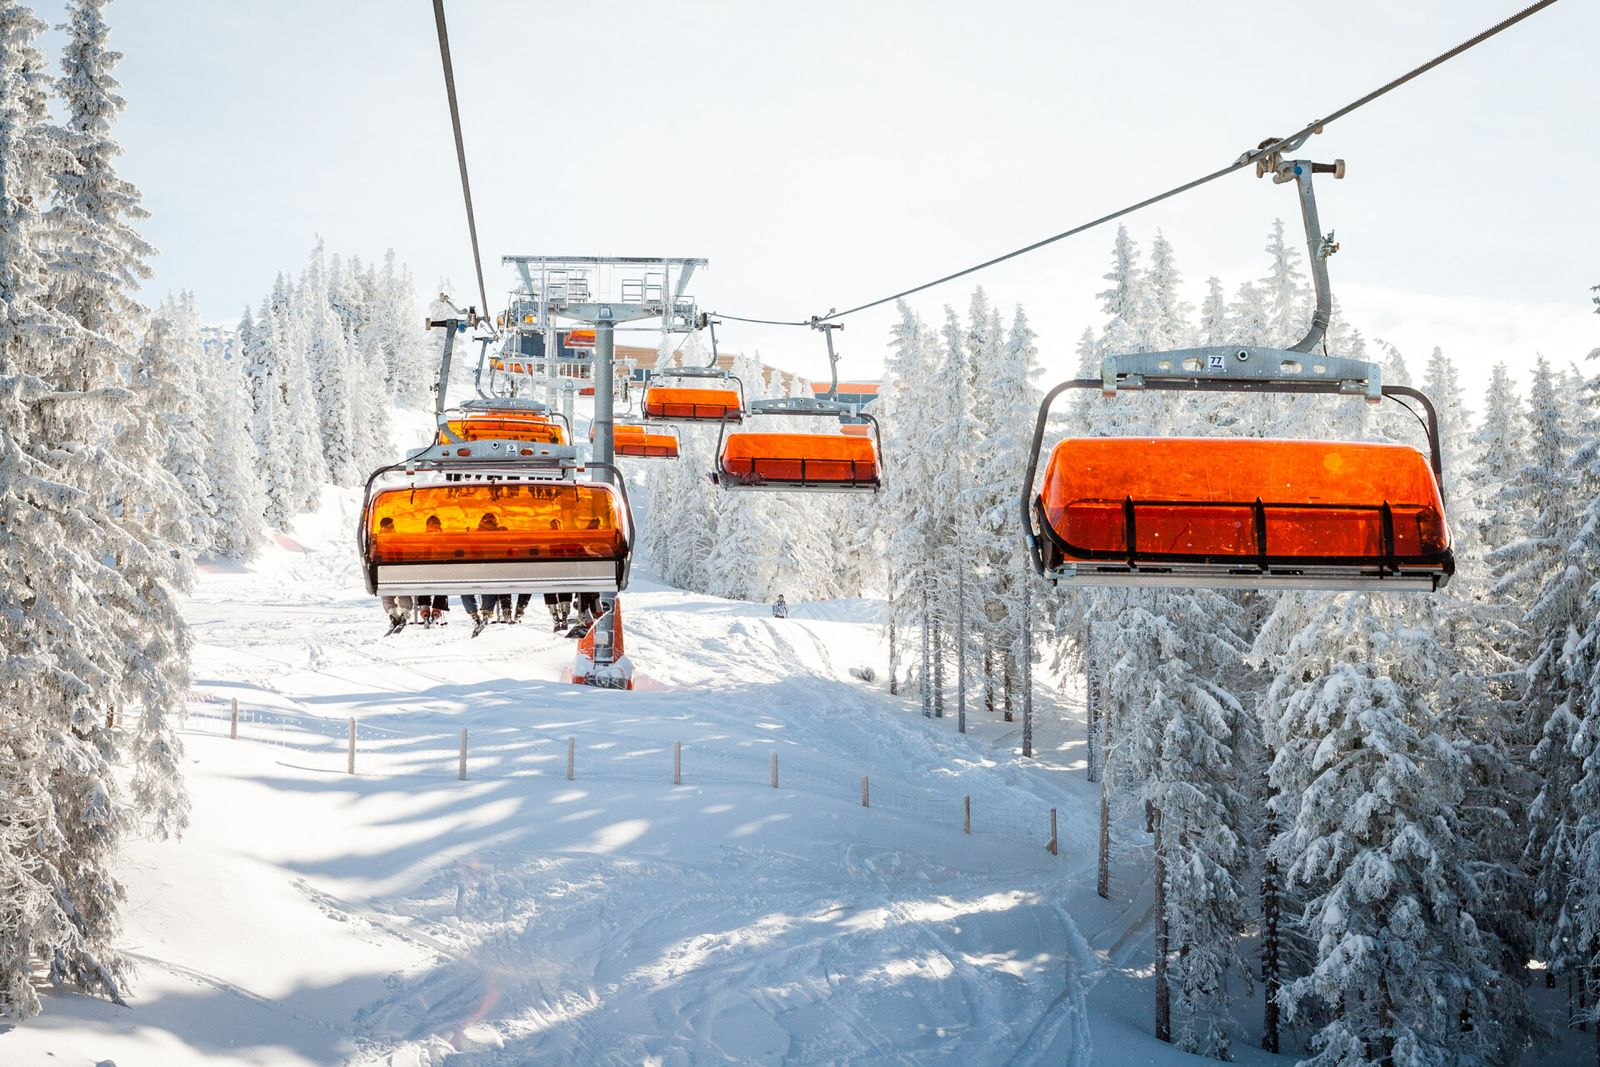
\includegraphics[width=0.5\linewidth]{ski.jpg}\par} Der alpenländische Warp-Antrieb in Aktion.\\
\hline
\noalign{\vskip 1mm}
\hline
% NICHT AUSFÜLLEN: Geben Sie an, wo die Arbeit eingesehen werden kann (physisch und digital). Nennen Sie Ansprechpartner und ggf. Kontaktinformationen.
Möglichkeit der Einsichtnahme in die Arbeit & Die Diplomarbeit ist in gebundener Form sowohl in der Schulbibliothek als auch bei AV Prof. Dipl-Ing. (FH) Roland Holzer einzusehen. Darüber hinaus besitzt jedes Mitglied des Projektteams eine vollständige Version in gebundener und digitaler Form.\\
\hline
\noalign{\vskip 1mm}
\hline
% NICHT AUSFÜLLEN: Unterschriftenfelder: Datum/Unterschrift, Prüfer/in, Abteilungsvorstand. Diese Felder bleiben leer und werden manuell unterschrieben.
\multicolumn{2}{|c|}{%
    \begin{tabular}{p{0.30\textwidth}|p{0.30\textwidth}|p{0.30\textwidth}}
        Approbation\newline(Datum/Unterschrift)\newline\newline & Prüfer/Prüferin & Abteilungsvorstand
    \end{tabular}
} \\
\hline
\end{tabular}

\newpage

\begin{center}
    {\fontsize{30}{36}\selectfont\bfseries Diploma Thesis}\\[0.5em]
    {\fontsize{20.74}{24}\selectfont\bfseries Documentation}
\end{center}
\vspace{0.5cm}
\noindent
\begin{tabular}{|p{0.31\textwidth}|p{0.61\textwidth}|}
\hline
% AUSFÜLLEN: Tragen Sie hier alle Autorennamen ein. Format: Vorname Nachname, ggf. mehrere durch Komma getrennt.
Author(s) & Felix Zauner, Timofey Luzin \\
\hline
% NICHT AUSFÜLLEN: Jahrgang/Schulform (z. B. 5AHET). Wenn nicht zutreffend, anpassen oder weglassen.
Form & 5AHET \\
% NICHT AUSFÜLLEN: Schuljahr im Format JJJJ/JJ (z. B. 2025/26).
Academic year & 2025/26  \\
\hline
% AUSFÜLLEN: Prägnanter Titel des Themas IN ENGLISCH. Sollte die Kernidee der Arbeit widerspiegeln.
Topic & ALBERT - Development of an Autonomous Guided Missile with Real-Time Attitude Control for Weather Data Collection \\
\hline
% AUSFÜLLEN: Externe Partner oder Firmen, die an der Arbeit beteiligt sind. Falls keine, "keine" oder leer lassen.
Cooperation Partners & Palfinger AG \\
\hline
\noalign{\vskip 1mm}
\hline
% AUSFÜLLEN: Hier die Aufgabenstellung IN ENGLISCH in ein paar Sätzen beschreiben.
Assignment & The assignment is the development of a prototype for a warp drive using modern propulsion technologies \\
\hline
\noalign{\vskip 1mm}
\hline
% AUSFÜLLEN: Beschreibung der Realisierung IN ENGLISCH. Hier sollte die Umsetzung des Projektes beschrieben werden.
Realization & A warp drive born of Alpine engineering relies less on physics and more on intuition, charm, and improvisation. Spacetime resembles a bumpy ski run, its energy supplied by a crate of beer and a great deal of persuasion. Calculations are produced as rhymed Gstanzln (folk verses) rather than in the laboratory. Thus the universe moves -- not by technology, but by creativity and the belief that even the cosmos can be softened with a smile.\\
\hline
\noalign{\vskip 1mm}
\hline
% AUSFÜLLEN: Konkrete Ergebnisse IN ENGLISCH zusammenfassen
Result & The developed warp drive enables interstellar journeys (Stubaital) to be completed in record time, with Alpine engineering providing a unique blend of efficiency and charm. Early tests indicate that the drive is not only functional but also has the potential to revolutionize the space industry. \\
\hline
\noalign{\vskip 1mm}
\hline
% AUSFÜLLEN: Fügen Sie hier die Bilddatei und eine kurze Bildunterschrift ein. Bilddateien sollten im gleichen Verzeichnis liegen oder mit Pfad angegeben werden.
Illustrative Graph, Photo (with explanation) & \vspace{0.1cm}{\centering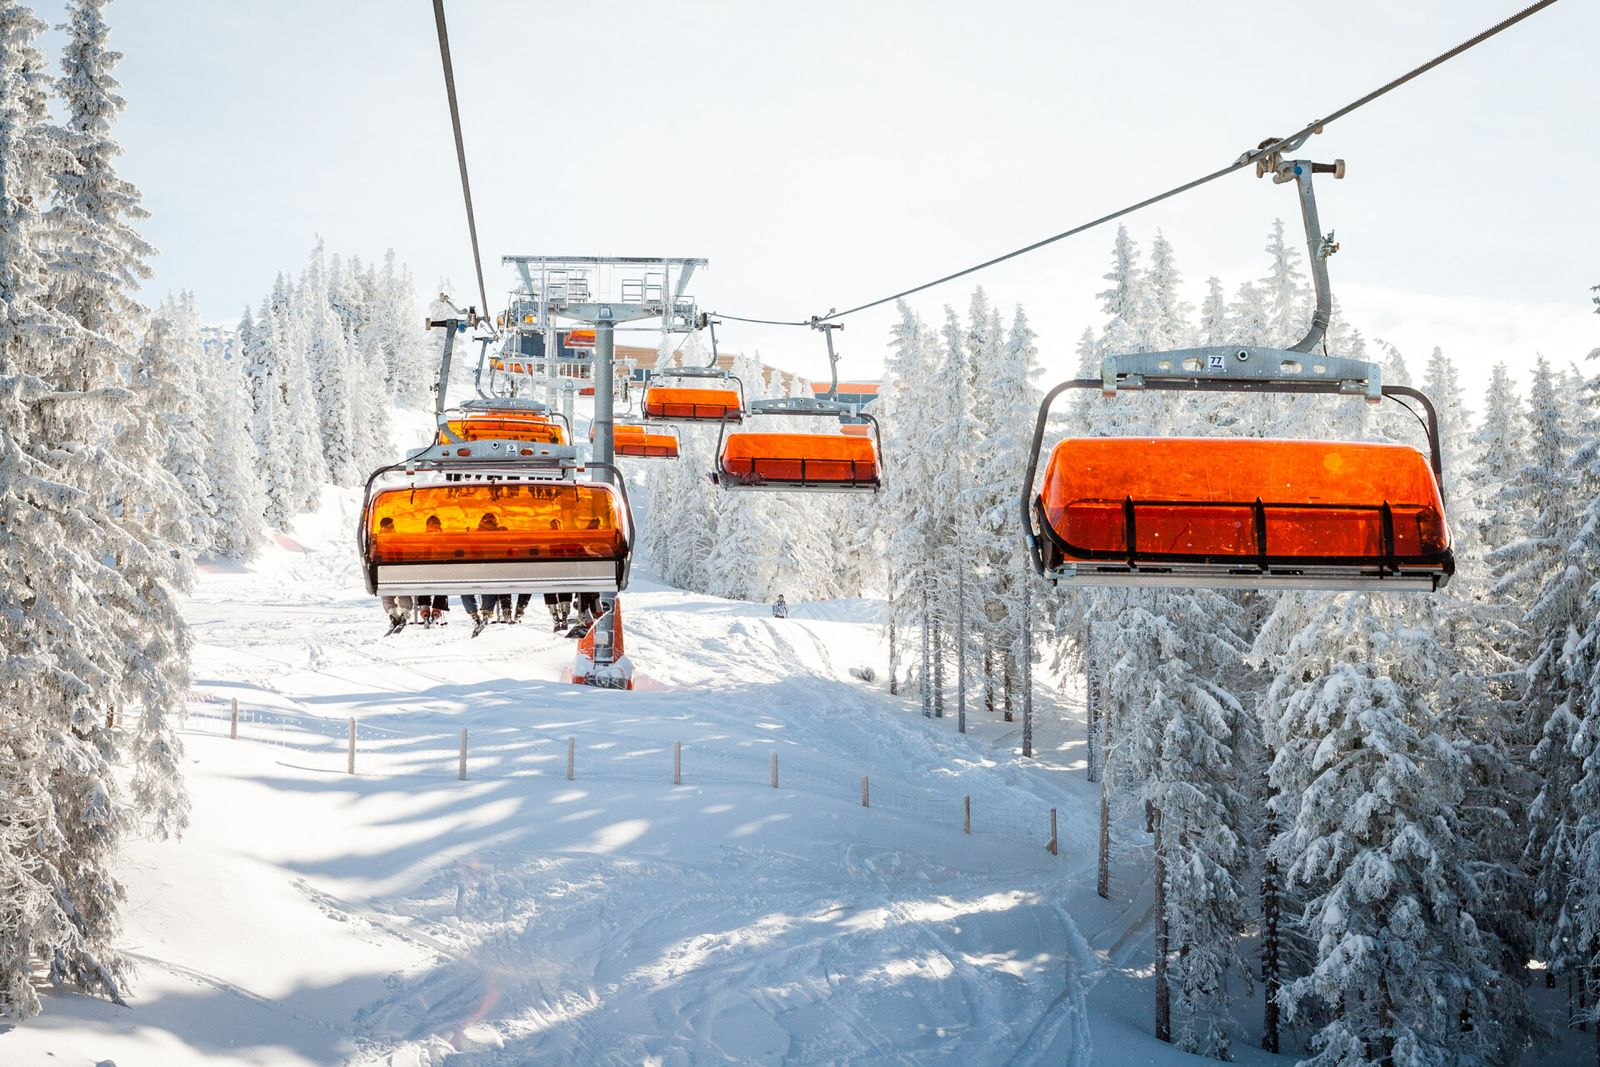
\includegraphics[width=0.5\linewidth]{ski.jpg}\par} The Alpine warp drive in action.\\
\hline
\noalign{\vskip 1mm}
\hline
% NICHT AUSFÜLLEN: Geben Sie an, wo die Arbeit eingesehen werden kann (physisch und digital). Nennen Sie Ansprechpartner und ggf. Kontaktinformationen.
Accessibility of \newline Diploma Thesis & The diploma thesis is available in the school library as well as in the office of the head of department Prof. Dipl-Ing. (FH) Roland Holzer. In addition, each member of the project team has a complete version in hardcover and digital form.\\
\hline
\noalign{\vskip 1mm}
\hline
% NICHT AUSFÜLLEN: Unterschriftenfelder: Datum/Unterschrift, Prüfer/in, Abteilungsvorstand. Diese Felder bleiben leer und werden manuell unterschrieben.
\multicolumn{2}{|l|}{%
    \begin{tabular}{p{0.30\textwidth}|p{0.30\textwidth}|p{0.30\textwidth}}
        Approval\newline(Date/Signature)\newline\newline &  Examiner & Head of Department
    \end{tabular}
} \\
\hline
\end{tabular}




%%%%%%%%%%%%%%%%%%%%%%%%%%%%%%%%%%%%%%%%%%%%%%%%%%%%%%%%%%%%%%%%%%%%%%%
%                   Anfang Verzeichnisse
%%%%%%%%%%%%%%%%%%%%%%%%%%%%%%%%%%%%%%%%%%%%%%%%%%%%%%%%%%%%%%%%%%%%%%%


%-------------------------------------------------------------------

% Verzeichnisse

\pagestyle{fancy} % Kopf- und Fußzeilen auch in Verzeichnissen aktivieren

\tableofcontents
\thispagestyle{fancy} 
\listoffigures 
\thispagestyle{fancy} % fancy-Stil für Abbildungsverzeichnis
\addcontentsline{toc}{chapter}{Abbildungsverzeichnis}
\cleardoublepage 
\listoftables
\thispagestyle{fancy} % fancy-Stil für Tabellenverzeichnis
\addcontentsline{toc}{chapter}{Tabellenverzeichnis}
\cleardoublepage

%%%%%%%%%%%%%%%%%%%%%%%%%%%%%%%%%%%%%%%%%%%%%%%%%%%%%%%%%%%%%%%%%%%%%%%
%                   Anfang Hauptteil
%%%%%%%%%%%%%%%%%%%%%%%%%%%%%%%%%%%%%%%%%%%%%%%%%%%%%%%%%%%%%%%%%%%%%%%

%neue Seite, damit die nächste Seite rechts ist
\thispagestyle{empty}
\cleardoublepage
\thispagestyle{fancy}
\pagenumbering{arabic} % Wechsel zu arabischer Nummerierung
\setcounter{page}{1} % Start bei 1
\fancyfoot[C]{\large Autor A}


% Bsp Abbildung

\section{Bsp Abbildung}

\begin{figure}[htbp]
    \centering
    
\includegraphics[width=0.8\textwidth]{HTL.png}
    \caption[Abbildung]{Beschreibung der Abbildung}
    \label{fig:eindeutige-bezeichnung}
\end{figure}

%-------------------------------------------------------------------

% Bsp Tabelle

\section{Bsp Tabelle}
\begin{table}[htbp]
    \centering
    \caption{Beschreibung der Tabelle}
    \label{tab:eindeutige-bezeichnung2}
    \vspace{0.5cm}
    \begin{tabular}{|l|c|r|}
        \hline
        Spalte 1 & Spalte 2 & Spalte 3 \\
        \hline
        Wert 1 & Wert 2 & Wert 3 \\
        \hline
    \end{tabular}
\end{table}

%-------------------------------------------------------------------

\section{Bespiel Text Referenz}
Siehe Abbildung \ref{fig:eindeutige-bezeichnung} auf Seite \pageref{fig:eindeutige-bezeichnung}.
Tabelle \ref{tab:eindeutige-bezeichnung2} zeigt die Ergebnisse.

\cleardoublepage

%%%%%%%%%%%%%%%%%%%%%%%%%%%%%%%%%%%%%%%%%%%%%%%%%%%%%%%%%%%%%%%
%                    Formeln
%%%%%%%%%%%%%%%%%%%%%%%%%%%%%%%%%%%%%%%%%%%%%%%%%%%%%%%%%%%%%%%

\section{Formeln im Fließtext und in eigener Zeile}

Formeln können im Fließtext oder abgesetzt dargestellt werden.

\subsection{Formel im Fließtext}

Beispiel einer Formel im Text:

\noindent Die Energie eines ruhenden Körpers wird durch $E = mc^2$ beschrieben...

\subsection{Formel in eigener Zeile (Display-Math)}

Die gleiche Formel abgesetzt und zentriert:

\[
E = mc^2
\]

\noindent oder mit automatischer Nummerierung:

\begin{equation}
E = mc^2
\end{equation}

\noindent Man kann mit einem Label darauf verweisen, zum Beispiel Gleichung~\eqref{eq:energie}:

\begin{equation}
E = mc^2
\label{eq:energie}
\end{equation}

% ==============================================================
\section{Gleichungssysteme}

Gleichungssysteme können auf verschiedene Arten dargestellt werden:
entweder als Block mit geschweiften Klammern oder als ausgerichtete Zeilen.

\subsection{Einfaches Gleichungssystem (ohne Ausrichtung)}

\[
\begin{cases}
x + y = 5 \\
x - y = 1
\end{cases}
\]

\subsection{Ausgerichtetes Gleichungssystem (mit \texttt{align})}

Hier werden die Gleichheitszeichen untereinander ausgerichtet:

\begin{align}
x + y &= 5 \\
x - y &= 1
\end{align}

\subsection{Gleichungssystem mit Beschriftung (Label)}

\noindent Das Label ermöglicht späteres Referenzieren.  
\noindent Beispiel: Siehe Gleichungssystem~\eqref{eq:gleichungssystem}.

\begin{align}
a + b &= 3 \\
2a - b &= 4
\label{eq:gleichungssystem}
\end{align}

\subsection{Ausrichtung mit mehreren Spalten (z.\,B. Zwischenschritte)}

\begin{align*}
x + y &= 5  && \text{(erste Gleichung)}\\
x - y &= 1  && \text{(zweite Gleichung)}\\
\Rightarrow\; 2x &= 6 && \text{(Addition)}\\
\Rightarrow\; x &= 3 && \text{(Division durch 2)}
\end{align*}

\subsection{Gleichungssystem mit einer gemeinsamen Nummer (split)}

\begin{equation}
\label{eq:split-system}
\begin{split}
x + y &= 5 \\
x - y &= 1
\end{split}
\end{equation}

\noindent Das obige System~\eqref{eq:split-system} wird als eine Einheit nummeriert.

% ==============================================================
\section{Laplace-Transformation}
\[
\mathcal{L}\{f(t)\} = F(s)
\]

\[
\begin{aligned}
f(t)\\
\TransformVert\\
F(s)
\end{aligned}
\]

% ==============================================================
\section{Matrix}
\noindent Ein Beispiel aus der Statistik:

% Darstellung mit runder Klammern
\[
A = \begin{pmatrix}
  a_{11} & a_{12} & a_{13} \\
  a_{21} & a_{22} & a_{23} \\
  a_{31} & a_{32} & a_{33}
\end{pmatrix}
\]

% Darstellung mit eckigen Klammern
\[
B = \begin{bmatrix}
  1 & 2 & 3 \\
  4 & 5 & 6 \\
  7 & 8 & 9
\end{bmatrix}
\]

% Darstellung mit geschwungener Klammern
\[
C = \left\{
\begin{matrix}
c_{11} & c_{12} & c_{13} \\
c_{21} & c_{22} & c_{23} \\
c_{31} & c_{32} & c_{33}
\end{matrix}
\right\}
\]

% ==============================================================
\section{Sonderzeichen und Operatoren}

\[
\begin{aligned}
x^2, \quad a_i, \quad \frac{a}{b}, \quad \sqrt{x}, \quad \sqrt[3]{y}, \\ % Potenz, Index, Bruch, Quadratwurzel, Kubikwurzel
\sum_{i=1}^n i^2, \quad \int_0^\infty e^{-x}\,dx, \quad % Summe, uneigentliches Integral (mit kleinem Abstand vor dx)
\lim_{x\to0} \frac{\sin x}{x}, \\ % Limes
\vec{a}, \quad \overrightarrow{AB}, \quad |x|, \quad \lvert x \rvert % Vektornotationen, Betrag (zwei Schreibweisen)
\end{aligned}
\]

% ==============================================================
\section{Kleine griechische Buchstaben im Fließtext}

Hier einige Beispiele für kleine griechische Buchstaben im Text:

\noindent $\alpha, \beta, \gamma, \delta, \epsilon, \zeta, \eta, \theta, \iota, \kappa, \lambda, \mu, \nu, \xi, \pi, \rho, \sigma, \tau, \phi, \chi, \psi, \omega$.

\noindent Beispielhafte Verwendung im Kontext:

\noindent Die Dichte $\rho$ eines Körpers und der Winkel $\theta$ sind wichtige Größen in der Physik.

% ==============================================================
\section{Große griechische Buchstaben in Gleichungen}

In der Mathematik werden auch große griechische Buchstaben verwendet:

\[
\Gamma + \Delta + \Theta = \Lambda + \Pi + \Sigma + \Omega
\] 



% ==============================================================
\section{Beispielhafte Formeln mit griechischen Symbolen}


\subsection{Beispiel aus der Trigonometrie}

\[
\sin(\alpha) + \cos(\beta) = 1
\]

\subsection{Beispiel aus der Physik}

\[
F = m \cdot g = m \cdot 9.81~\frac{\text{m}}{\text{s}^2}
\]

\noindent mit dem Winkelbezug $\theta$:
\[
F_\text{Hang} = F \cdot \sin(\theta)
\]

% ==============================================================
\section{Übersicht: Griechische Buchstaben in \LaTeX}

\begin{center}
\begin{tabular}{ll|ll}
\textbf{Klein} & \textbf{Code} & \textbf{Groß} & \textbf{Code} \\
\hline
$\alpha$ & \verb|\alpha| & $\Gamma$ & \verb|\Gamma| \\
$\beta$ & \verb|\beta| & $\Delta$ & \verb|\Delta| \\
$\gamma$ & \verb|\gamma| & $\Theta$ & \verb|\Theta| \\
$\delta$ & \verb|\delta| & $\Lambda$ & \verb|\Lambda| \\
$\epsilon$ & \verb|\epsilon| & $\Xi$ & \verb|\Xi| \\
$\zeta$ & \verb|\zeta| & $\Pi$ & \verb|\Pi| \\
$\eta$ & \verb|\eta| & $\Sigma$ & \verb|\Sigma| \\
$\theta$ & \verb|\theta| & $\Upsilon$ & \verb|\Upsilon| \\
$\lambda$ & \verb|\lambda| & $\Phi$ & \verb|\Phi| \\
$\mu$ & \verb|\mu| & $\Psi$ & \verb|\Psi| \\
$\nu$ & \verb|\nu| & $\Omega$ & \verb|\Omega| \\
$\xi$ & \verb|\xi| & & \\
$\pi$ & \verb|\pi| & & \\
$\rho$ & \verb|\rho| & & \\
$\sigma$ & \verb|\sigma| & & \\
$\tau$ & \verb|\tau| & & \\
$\phi$ & \verb|\phi| & & \\
$\chi$ & \verb|\chi| & & \\
$\psi$ & \verb|\psi| & & \\
$\omega$ & \verb|\omega| & & \\
\end{tabular}
\end{center}

% ==============================================================
\section{Mengenzeichen}

Die wichtigsten Zahlenmengen der Mathematik werden mit Doppelstrich-Buchstaben dargestellt.  
Dazu verwendet man in \LaTeX{} den Befehl \verb|\mathbb|{} (bereitgestellt durch das Paket \texttt{amssymb}).

\[
\mathbb{N}, \mathbb{Z}, \mathbb{Q}, \mathbb{R}, \mathbb{C}
\]

\begin{itemize}
    \item $\mathbb{N}$ – Menge der natürlichen Zahlen
    \item $\mathbb{Z}$ – Menge der ganzen Zahlen
    \item $\mathbb{Q}$ – Menge der rationalen Zahlen
    \item $\mathbb{R}$ – Menge der reellen Zahlen
    \item $\mathbb{C}$ – Menge der komplexen Zahlen
\end{itemize}

%%%%%%%%%%%%%%%%%%%%%%%%%%%%%%%%%%%%%%%%%%%%%%%%%%%%%%%%%%%%%%%%%%%%%%
%                   ANFANG Schaltkreise
%%%%%%%%%%%%%%%%%%%%%%%%%%%%%%%%%%%%%%%%%%%%%%%%%%%%%%%%%%%%%%%%%%%%%%

\newpage % Neue Seite nach Titelseite


\section{Einleitung} % Abschnitt: Einführung

% Kurze Beschreibung, was circuitikz ist und wofür es verwendet wird
Circuitikz ist ein LaTeX-Paket welches verwendet wird, um elektrische und elektronische Schaltpläne direkt in LaTeX zu zeichnen. Es stellt eine Sammlung von Symbolen und Befehlen bereit, um Widerstände, Kondensatoren, Transistoren, Spannungsquellen usw. einfach zu zeichnen.

\subsection{Package}
% Erklärung, wie das Paket eingebunden wird
Um das circuitikz-Paket in LaTeX zu verwenden, muss es zuerst importiert werden.
Das geschieht im Vorspann, vor \\begin{document} des LaTeX-Dokuments mit der Zeile: \\usepackage{circuitikz}.

\section{Schaltungen zeichnen}

\subsection{TikZ}
% circuitikz basiert auf TikZ – wichtig für das Verständnis der Syntax
circuitikz basiert auf TikZ, einem weiteren LaTeX-Paket, das sich mit dem Zeichnen von Grafiken befasst. Um circuitikz besser zu verstehen, sollte man sich zunächst mit TikZ vertraut machen, da einige Funktionen und Befehle auf die gleiche Weise verwendet werden.

\subsection{Linie}
% Grundelement: Linien verbinden Schaltungselemente
In circuitikz beginnt man immer mit einer Linie, weil alle Schaltungselemente an Liniensegmenten zwischen zwei Punkten platziert werden. Diese kann entwerder mit der Zeile \\draw (0,0) -- (2,0); oder mit \\draw (0,0) to (2,0); ausgefürt werden.

\begin{center}
\begin{circuitikz}
    \draw (0,0) -- (2,0); % Zeichnet eine einfache horizontale Linie
\end{circuitikz}
\end{center}

\subsection{Schaltungselemente}
% Beispiel: Widerstand zwischen zwei Punkten
Um ein Schaltungselement einzufügen und mit einer Linie zu verbinden, muss man die Zeile einfach zu \\draw (0,0) to[resistor] (2,0); ändern.

\begin{center}
\begin{circuitikz}
    \draw (0,0) to[resistor] (2,0); % Fügt einen Widerstand ein
\end{circuitikz}
\end{center}

% Hinweis: Viele Bauteile lassen sich direkt mit einem Schlüsselwort verwenden
Viele elektrische Schaltungselemente könne, so wie der Widerstand, einfach mit einem Wort eingefügt werden.

\subsubsection{Monopole}
% Monopole = Bauteile mit nur einem Anschluss (z. B. Ground)

\newcommand{\thiscirc}[1]{%
\texttt{#1}\kern5pt\hfill
\begin{circuitikz}%
\draw (0,0) node[ #1 ] {}; % Zeichnet Symbol als einzelnes Node
\end{circuitikz}%
{\hspace{5mm}}%
}

% Tabelle mit verschiedenen Monopolen
\renewcommand{\arraystretch}{2}
\begin{center}
\begin{tabular}{lll} 
\thiscirc{ground} & \thiscirc{sground} & \thiscirc{nground}\\
\thiscirc{rground} & \thiscirc{pground} & \thiscirc{cground}\\
\thiscirc{tlinestub} & \thiscirc{antenna} & \thiscirc{rxantenna}\\
\end{tabular}
\end{center}

% Erklärung: Monopole werden mit "node" platziert
Ein Monopol kann nur dann eingefügt werden wenn man den befehl "node", dann den namen des Monopls und dann erst die zweite Koordinate einfügt. z.B. \\draw (0,0) node[ground]{} to (0,0); 

\begin{center}
\begin{circuitikz}
  \draw (0,0) node[ground]{} to (0,0); % Ground-Symbol an Position (0,0)
\end{circuitikz}
\end{center}

% Einfacher Stromkreis mit Ground, Spannungsquelle und Widerstand
\begin{center}
\begin{circuitikz}
  \draw (0,0) node[ground]{} to (0,0); 
  \draw (0,0) to[V, l=$U$] (0,3);
  \draw (0,3) to[R, l=$R$] (3,3);
  \draw (3,3) to (3,0);
  \draw (3,0) to (0,0);
\end{circuitikz}
\end{center}

\subsubsection{Bipole}
% Bipole: Bauteile mit zwei Anschlüssen (z. B. Widerstände, Dioden, Spulen)

\newcommand{\bipole}[1]{%
\texttt{#1}\kern5pt \hfill
\begin{circuitikz}%
\draw (0,0) to[ #1 ] (2,0); % Zeichnet Bipol zwischen zwei Punkten
\end{circuitikz}%
\hspace{5mm}%
}

% Übersicht gängiger Bipole
\renewcommand{\arraystretch}{3}
\begin{center}
\begin{tabular}{ll} 
\bipole{ammeter} & \bipole{voltmeter} \\
\bipole{short} & \bipole{open} \\
\bipole{lamp} & \bipole{generic} \\
\bipole{tgeneric} & \bipole{ageneric} \\
\bipole{fullgeneric} & \bipole{tfullgeneric} \\
\bipole{memristor} & \bipole{american resistor} \\
\bipole{vR} & \bipole{american potentiometer} \\
\bipole{european resistor} & \bipole{european potentiometer} \\
\bipole{varistor} & \bipole{photoresistor} \\
\bipole{thermocouple} & \bipole{thermistor} \\
\bipole{thermistor ntc} & \bipole{fuse} \\
\bipole{afuse} & \bipole{battery} \\
\bipole{battery1} & \bipole{european voltage source} \\
\bipole{american voltage source} & \bipole{european current source} \\
\bipole{american current source} &  \\
\end{tabular}
\end{center}

\subsubsection{Dioden}
% Neue Tabelle: verschiedene Diodentypen
\renewcommand{\bipole}[1]{%
\texttt{#1}\kern5pt \hfill
\begin{circuitikz}%
\draw (0,0) to[ #1 ] (2,0); 
\end{circuitikz}%
\hspace{5mm}%
}

\renewcommand{\arraystretch}{3}
\begin{center}
\begin{tabular}{ll} 
\bipole{empty diode} & \bipole{empty Schottky diode} \\
\bipole{empty Zener diode} & \bipole{empty tunnel diode} \\
\bipole{photodiode} & \bipole{empty diode} \\
\bipole{empty varcap} & \bipole{full diode} \\
\bipole{full Schottky diode} & \bipole{full Zener diode} \\
\bipole{full tunnel diode} & \bipole{full photodiode} \\
\bipole{full led} & \bipole{full varcap} \\
\bipole{squid} & \bipole{barrier} \\
\end{tabular}
\end{center}

\subsubsection{Dynamische Bipole}
% Tabelle mit dynamischen Bauteilen wie Kondensator, Spule, Quelle etc.
\renewcommand{\bipole}[1]{%
\texttt{#1}\kern5pt \hfill
\begin{circuitikz}%
\draw (0,0) to[ #1 ] (2,0); 
\end{circuitikz}%
\hspace{5mm}%
}

\renewcommand{\arraystretch}{3}
\begin{center}
\begin{tabular}{ll} 
\bipole{capacitor} & \bipole{curved capacitor} \\
\bipole{variable capacitor} & \bipole{cute inductor} \\
\bipole{variable cute inductor} & \bipole{american inductor} \\
\bipole{variable american inductor} & \bipole{european inductor} \\
\bipole{variable european inductor} & \bipole{transmission line} \\
\bipole{vsourcesin} & \bipole{isourcesin} \\
\bipole{closing switch} & \bipole{opening switch} \\
\bipole{push button} & \\
\end{tabular}
\end{center}

% Hinweis auf Kurzformen von Symbolen
Für manche Bauteile gibt es auch abkürzungen. So wie V für Spannungsquelle oder R für Widerstand oder L für Spulen.

\subsection{Europäisch/Amerekanisch}
% Erklärung der Symbolstile: europäisch oder amerikanisch
In circuitikz kann man zwischen europäischen und amerikanischen Schaltsymbolen wählen. Dies kann man entweder dadurch steuern, dass man european oder american vor die Bezeichnung des Schaltelements schreibt, z.B. \\bipole{european resistor} oder \\bipole{american resistor} oder indem man den gesamten Schaltplan auf europäische oder amerikanische Symbole setzt. \\begin{circuitikz}[american] 

\begin{center}
\begin{circuitikz}[american] 
    \draw (0,0) to[resistor] (2,0); % Amerikanische Darstellung
\end{circuitikz}
\end{center}

\begin{center}
\begin{circuitikz}[european] 
    \draw (0,0) to[resistor] (2,0); % Europäische Darstellung
\end{circuitikz}
\end{center}

\subsection{Bezeichnung}
% Beschriftung von Bauteilen (Label)
Ein Schaltelement wird benannt, indem man die Zeile \\draw (0,0) to[resistor] (2,0); auf \\draw (0,0) to[resistor, l=$R$] (2,0); ändert. Damit wird ein Label (Beschriftung) R am Bauteil angezeigt.

\begin{center}
\begin{circuitikz}[european] 
    \draw (0,0) to[resistor, l=$R$] (2,0); % Label oberhalb
\end{circuitikz}
\end{center}

\begin{center}
\begin{circuitikz}[european] 
    \draw (0,0) to[resistor, l_=$R$] (2,0); % Label unterhalb
\end{circuitikz}
\end{center}

\subsection{Ströme/Spannungen}
% Darstellung von Strom- und Spannungspfeilen

\subsubsection{Ströme}
% Strompfeile (i=$i$)
Ströme werden mithilfe der Zeile \\draw (0,0) to[short, i=$i$] (2,0); dargestellt. 

\begin{center}
\begin{circuitikz}[european] 
    \draw (0,0) to[short, i=$i$] (2,0); % Strom von links nach rechts
\end{circuitikz}
\end{center}

\begin{center}
\begin{circuitikz}[european] 
    \draw (2,0) to[short, i_=$i$] (0,0); % Strom von rechts nach links
\end{circuitikz}
\end{center}

\subsubsection{Spannungen}
% Spannungspfeile (v^>=$U$)
Spannungen werden mithilfe der Zeile \\draw (0,0) to[open, vHoch>=$U$] (2,0); dargestellt.

\begin{center}
\begin{circuitikz}[european] 
    \draw (0,0) to[open, v^>=$U$] (2,0); % Spannung von links nach rechts
\end{circuitikz}
\end{center}

\begin{center}
\begin{circuitikz}[european] 
    \draw (2,0) to[open, v^>=$U$] (0,0); % Spannung von rechts nach links
\end{circuitikz}
\end{center}

\subsection{Schaltung}

\subsubsection{Leitungen}
% Beispiel für Leitungsverbindungen (Rahmen)
\begin{center}
\begin{circuitikz}[european] 
    \draw (0,0) to (6,0);
    \draw (6,0) to (6,4);
    \draw (6,4) to (0,4);
\end{circuitikz}
\end{center}

\subsubsection{Schaltungselemente}
% Beispielschaltung mit Spannungsquelle, Widerstand und Spule
\begin{center}
\begin{circuitikz}[european] 
    \draw (0,0) to (6,0);
    \draw (6,0) to[V, l=$U$] (6,4);
    \draw (6,4) to[R, l=$R$] (3,4);
    \draw (3,4) to[L, l=$L$] (0,4);
\end{circuitikz}
\end{center}

\subsubsection{Spannungen/Ströme}
% Erweiterte Schaltung mit Strom- und Spannungspfeilen
\begin{center}
\begin{circuitikz}[european] 
    \draw (0,0) to[short, *-] (6,0);
    \draw (6,0) to[V, l=$U$] (6,4);
    \draw (6,4) to[R, l=$R$] (3,4);
    \draw (3,4) to[L, l=$L$] (1,4);
    \draw (0,4) to[short, *-, i=$i$] (1,4);
    \draw (0,0) to[open, v^>=u] (0,4);
\end{circuitikz}
\end{center}

\section{Beispiel}
% Komplexeres Beispiel mit mehreren Strom- und Spannungspfaden
\begin{center}
\begin{circuitikz}[european]
\draw
  (0,0) to [short, *-] (6,0)
  to [V, l_=$\mathrm{j}{\omega}_m \underline{\psi}^s_R$] (6,2) 
  to [R, l_=$R_R$] (6,4) 
  to [short, i_=$\underline{i}^s_R$] (5,4) 
  (0,0) to [open, v^>=$\underline{u}^s_s$] (0,4) 
  to [short, *- ,i=$\underline{i}^s_s$] (1,4) 
  to [R, l=$R_s$] (3,4)
  to [L, l=$L_{\sigma}$] (5,4) 
  to [short, i_=$\underline{i}^s_M$] (5,3) 
  to [L, l_=$L_M$] (5,0); 
\end{circuitikz}
\end{center}

\section{Website}
% Hinweis auf die Online-Plattform circuit2tikz zur grafischen Erstellung von Schaltungen
Um das Erstellen von Schaltungen zu erleichtern, kann auch die Website
https://www.circuit2tikz.tf.fau.de/designer/ verwendet werden. Dort kann eine Schaltung – ähnlich wie in Programmen wie S-Plan oder E-Plan – per Drag-and-Drop erstellt werden. Anschließend lässt sich der erzeugte LaTeX-Code extrahieren und direkt in das eigene Dokument einfügen.

\subsection{Schaltung zeichnen}

% Screenshot des User Interface
\begin{center}
\begin{figure}[h]
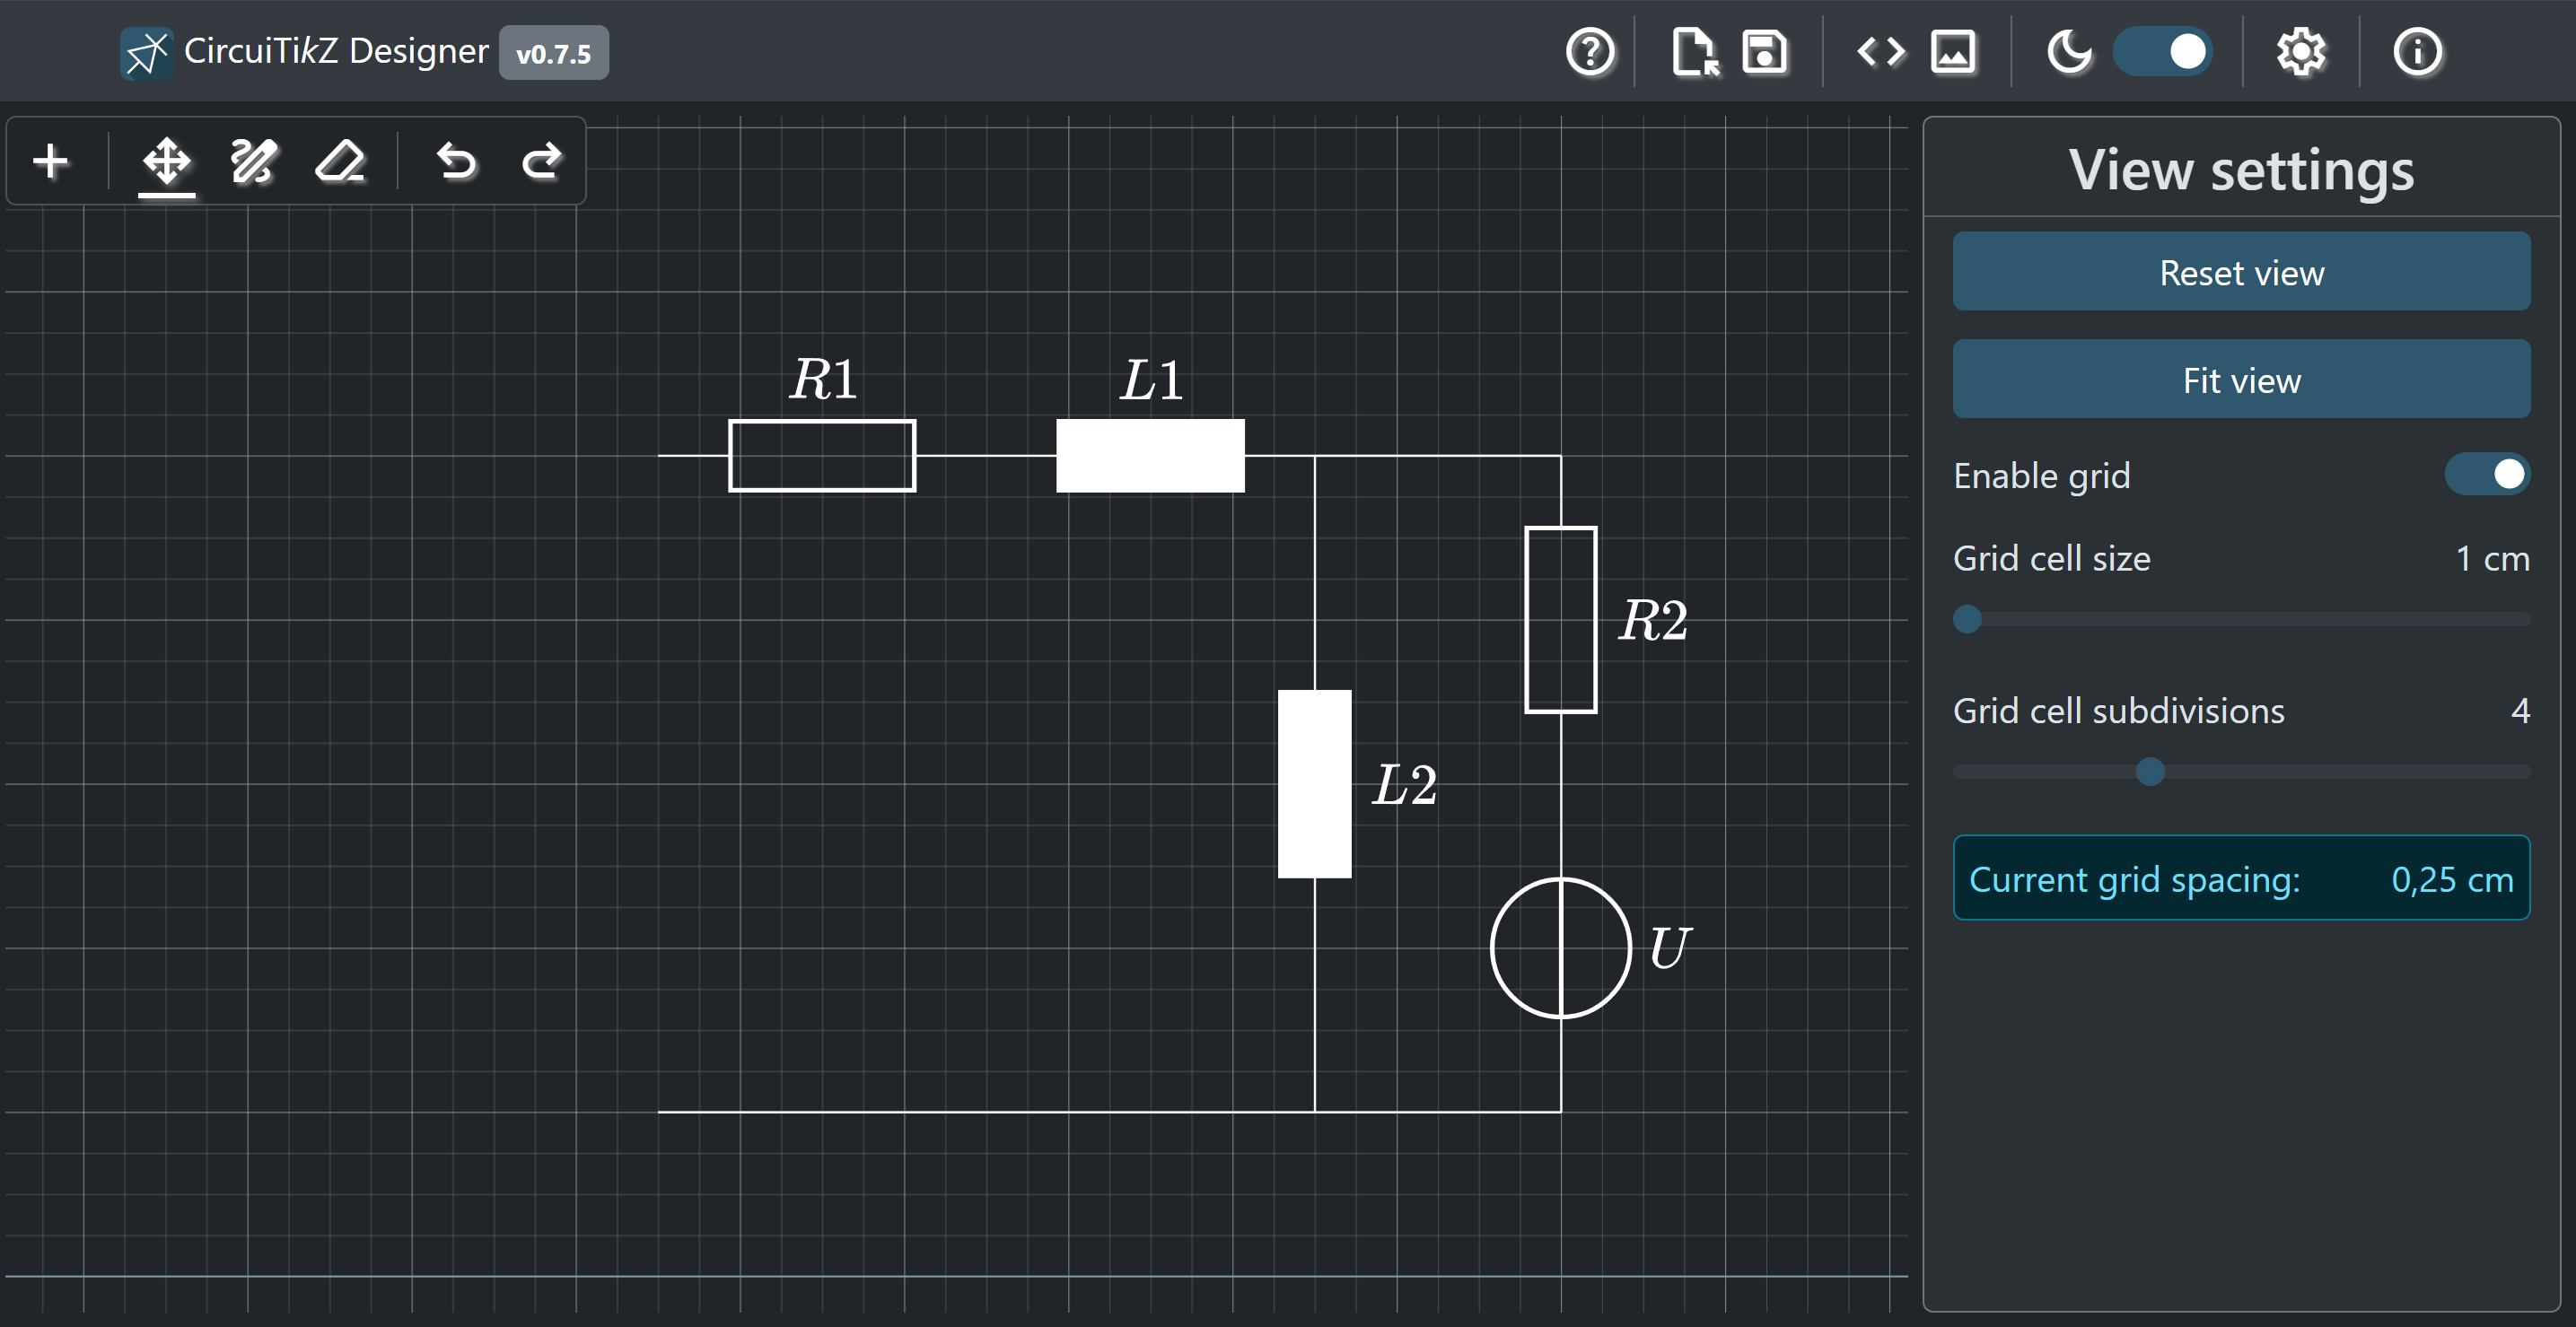
\includegraphics[scale=0.4]{website1.PNG}
\caption{User Interface}
\label{User Interface}
\end{figure} 
\end{center}

% Beispiel: TikZ-Schaltungscode aus der Website
\begin{center}
\begin{tikzpicture}
	% Pfade, Nodes und Verbindungen
	\draw (5.5, 5) to[european resistor, l={$R1$}] (7.5, 5); % Widerstand R1
	\draw (7.5, 5) to[european inductor, l={$L1$}] (9.5, 5); % Spule L1
	\draw (11, 5) to[european resistor, l={$R2$}] (11, 3); % Widerstand R2
	\draw (11, 3) to[european voltage source, l={$U$}] (11, 1); % Spannungsquelle U
	\draw (9.5, 5) to[european inductor, l={$L2$}] (9.5, 1); % Spule L2
	\draw (9.5, 5) -- (11, 5); % Verbindung oben
	\draw (11, 1) |- (5.5, 1); % Verbindung unten
\end{tikzpicture}
\end{center}

% Hinweis zum Abrufen des LaTeX-Codes von der Website
Auf den erzeugten LaTeX-Code kann durch einen Klick auf die Pfeile in der oberen rechten Ecke zugegriffen werden. Der Code muss nur kopiert und eingefügt werden.

% Screenshot: LaTeX-Code der Website
\begin{center}
\begin{figure}[h]
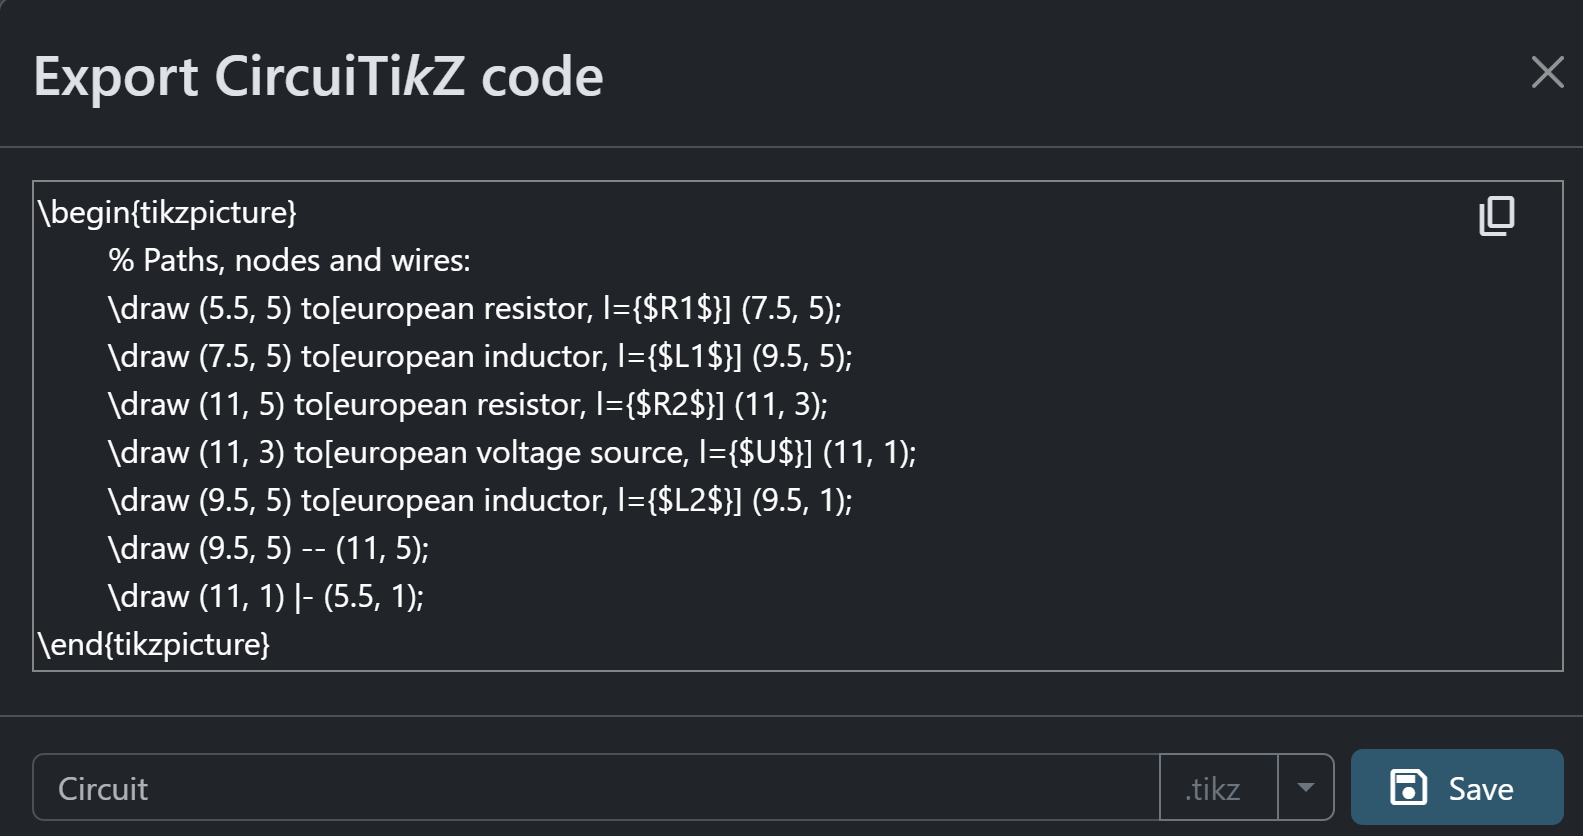
\includegraphics[scale=0.6]{website 2.PNG} % Screenshot Code
\caption{LaTeX Code}
\label{LaTex Code}
\end{figure} 
\end{center}


%%%%%%%%%%%%%%%%%%%%%%%%%%%%%%%%%%%%%%%%%%%%%%%%%%%%%%%%%%%%%%%%%%%%%%%%%%%%%%%
%                              Flowcharts und Diagramme
%%%%%%%%%%%%%%%%%%%%%%%%%%%%%%%%%%%%%%%%%%%%%%%%%%%%%%%%%%%%%%%%%%%%%%%%%%%%%%%





\cleardoublepage

%%%%%%%%%%%%%%%%%%%%%%%%%%%%%%%%%%%%%%%%%%%%%%%%%%%%%%%%%%%%%%%%%%%%%%%%%%%%%%%
\section{Liniendiagramm aus CSV-Daten mit \texttt{pgfplots}}
%%%%%%%%%%%%%%%%%%%%%%%%%%%%%%%%%%%%%%%%%%%%%%%%%%%%%%%%%%%%%%%%%%%%%%%%%%%%%%%

\subsection{Einleitung}
In diesem Abschnitt wird gezeigt, wie mit \LaTeX{} und dem Paket \texttt{pgfplots}
ein Liniendiagramm aus einer externen CSV-Datei erstellt wird.  
Die Codeausschnitte werden farbig dargestellt und anschließend das fertige Diagramm gezeigt.

\subsection{Vorbereitung der Daten}
Die zu visualisierenden Daten liegen in einer CSV-Datei vor.  
Ihr Inhalt sieht wie folgt aus:

\begin{lstlisting}[
    style=csvstyle,
    caption={Inhalt der Datei \texttt{../ZCSV/daten.csv}},
    label=lst:csv
]
x,y
0,1
1,2
2,4
3,3
4,5
5,7
\end{lstlisting}

\noindent
Die erste Zeile enthält die Spaltenüberschriften \texttt{x} und \texttt{y}.  
Jede weitere Zeile stellt ein Messpaar dar, das als Punkt im Diagramm visualisiert wird.

\subsection{Einlesen und Plotten der Daten}
Der zentrale Befehl zum Einlesen der CSV-Daten ist \texttt{\textbackslash addplot} in Kombination mit \texttt{table}.

\begin{lstlisting}[
    style=latexstyle,
    caption={Plotten der Daten aus einer CSV-Datei},
    label=lst:addplot
]
\addplot[
    blue,
    mark=*,
    line width=1pt
] table [
    col sep=comma,
    x=x,
    y=y
] {../ZCSV/daten.csv};
\end{lstlisting}

\noindent
Hier wird die Datei \texttt{../ZCSV/daten.csv} eingelesen, wobei die Spalte \texttt{x} auf die X-Achse
und die Spalte \texttt{y} auf die Y-Achse abgebildet wird.

\subsection{Vollständiges Diagramm}
Das folgende Listing zeigt die gesamte \texttt{axis}-Umgebung:

\begin{lstlisting}[
    style=latexstyle,
    caption={Komplette \texttt{axis}-Umgebung für das Liniendiagramm},
    label=lst:axis
]
\begin{tikzpicture}
  \begin{axis}[
    title={Liniendiagramm aus \texttt{../ZCSV/daten.csv}},
    xlabel={X-Werte},
    ylabel={Y-Werte},
    grid=major,
    legend pos=north west,
    width=12cm,
    height=8cm,
    xmin=0, xmax=5,
    ymin=0, ymax=8,
    thick
  ]
  
  \addplot[
    blue,
    mark=*,
    line width=1pt
  ] table [
    col sep=comma,
    x=x,
    y=y
  ] {../ZCSV/daten.csv};
  
  \legend{Messreihe}
  \end{axis}
\end{tikzpicture}
\end{lstlisting}

\noindent
Die Umgebung \texttt{axis} definiert das Koordinatensystem.  
Parameter wie \texttt{grid}, \texttt{width}, \texttt{height} oder \texttt{legend pos}
bestimmen Darstellung und Layout.

\subsection{Ergebnis}
Das resultierende Diagramm ist in Abbildung~\ref{fig:lineplot} dargestellt.

\begin{center}
\begin{tikzpicture}
  \begin{axis}[
    title={Liniendiagramm aus \texttt{../ZCSV/daten.csv}},
    xlabel={X-Werte},
    ylabel={Y-Werte},
    grid=major,
    legend pos=north west,
    width=12cm,
    height=8cm,
    xmin=0, xmax=5,
    ymin=0, ymax=8,
    thick
  ]
  \addplot[
    blue,
    mark=*,
    line width=1pt
  ] table [
    col sep=comma,
    x=x,
    y=y
  ] {../ZCSV/daten.csv};
  \legend{Messreihe}
  \end{axis}
\end{tikzpicture}
\end{center}
\label{fig:lineplot}

%%%%%%%%%%%%%%%%%%%%%%%%%%%%%%%%%%%%%%%%%%%%%%%%%%%%%%%%%%%%%%%%%%%%%%%%%%%%%%%
\section{Flowchart der Ball Balancing Platform (BBP) mit \texttt{TikZ}}
%%%%%%%%%%%%%%%%%%%%%%%%%%%%%%%%%%%%%%%%%%%%%%%%%%%%%%%%%%%%%%%%%%%%%%%%%%%%%%%

\subsection{Einleitung}
Im zweiten Teil wird gezeigt, wie mit dem Paket \texttt{TikZ} ein vollständiges
Flowchart für die Softwaresteuerung der Ball Balancing Platform (BBP) erstellt wird.
Das Diagramm bildet den Programmablauf des Regelkreises ab.

\subsection{Definition der TikZ-Styles}
Die grafischen Styles bestimmen Form, Farbe und Textausrichtung der Blöcke.

\begin{lstlisting}[
    style=latexstyle,
    caption={Definition der Styles für das Flowchart},
    label=lst:styles
]
\tikzstyle{startstop} = [rectangle, rounded corners, minimum width=3cm,
 minimum height=1cm, text centered, text width=3cm,
 draw=black, fill=red!20]
\tikzstyle{process} = [rectangle, minimum width=3cm, minimum height=1cm,
 text centered, text width=3cm, draw=black, fill=orange!20]
\tikzstyle{decision} = [diamond, minimum width=3cm, minimum height=1cm,
 text centered, draw=black, fill=green!20, aspect=1]
\tikzstyle{io} = [trapezium, trapezium left angle=70, trapezium right angle=110,
 minimum width=3.5cm, minimum height=1cm,
 text centered, text width=2cm, draw=black, fill=blue!20]
\tikzstyle{arrow} = [thick, ->, >=stealth]
\end{lstlisting}

\subsection{Erstellung der Knoten}
Jede Funktionseinheit wird durch einen \texttt{node}-Befehl dargestellt.  
Die Positionierung erfolgt relativ zu anderen Knoten.

\begin{lstlisting}[
    style=latexstyle,
    caption={Definition der Knoten für das Flowchart},
    label=lst:nodes
]
\node(start) [startstop] {Start};
\node(homing) [process, below of=start] {Homing};
\node(control_loop) [process, below of=homing] {Control Loop};
\node(camera) [io, below of=control_loop] {Read Camera};
\node(circle_detection) [process, below of=camera] {Circle Detection};
\node(read_mode) [io, below of=circle_detection] {Read Mode};
\node(mode1) [decision, below of=read_mode, yshift=-0.6cm] {Mode = 1?};
\node(mode2) [decision, below of=mode1, yshift=-1.2cm] {Mode = 2?};
\node(target_zero) [process, below of=mode2, yshift=-0.6cm] {Set Target = 0};
\node(read_joystick) [io, right of=mode1, xshift=6cm] {Read Joystick};
\node(target_circle) [process, right of=mode2, xshift=2cm] {Set Target = Circle()};
\node(calc_target) [process, right of=mode2, xshift=6cm] {Compute Target Value};
\node(pid) [process, below of=target_zero] {PID Control};
\node(invkin) [process, below of=pid] {Inverse Kinematics};
\node(motor_control) [io, below of=invkin] {Drive Motors};
\node(exit) [decision, below of=motor_control, yshift=-0.5cm] {Exit?};
\node(cleanup) [process, below of=exit, yshift=-0.5cm] {Cleanup};
\node(stop) [startstop, below of=cleanup] {Stop};
\end{lstlisting}

\subsection{Verbindungen und Pfeile}
Die logischen Verbindungen werden mit \texttt{\textbackslash draw[arrow]} erstellt.

\begin{lstlisting}[
    style=latexstyle,
    caption={Verbindungen der Blöcke mit Beschriftungen},
    label=lst:arrows
]
\draw[arrow] (mode1) -- (mode2)         node[anchor=west, midway] {No};
\draw[arrow] (mode1) -- (read_joystick) node[anchor=south, midway] {Yes};
\draw[arrow] (mode2) -- (target_zero)   node[anchor=west, midway] {No};
\draw[arrow] (mode2) -- (target_circle) node[anchor=south, midway] {Yes};
\draw[arrow] (target_circle) |- (pid);  % Knickpfad
\draw[arrow] (exit.east) -- node[anchor=south] {No} ++(10,0) |- (control_loop.east);
\end{lstlisting}

\subsection{Ergebnis}
Das fertige Flowchart ist in Abbildung~\ref{fig:flowchart} dargestellt.

\begin{center}
\begin{tikzpicture}[node distance=2cm, scale=.55, transform shape]
\node(start) [startstop] {Start};
\node(homing) [process, below of=start] {Homing};
\node(control_loop) [process, below of=homing] {Control Loop};
\node(camera) [io, below of=control_loop] {Read Camera};
\node(circle_detection) [process, below of=camera] {Circle Detection};
\node(read_mode) [io, below of=circle_detection] {Read Mode};
\node(mode1) [decision, below of=read_mode, yshift=-0.6cm] {Mode = 1?};
\node(mode2) [decision, below of=mode1, yshift=-1.2cm] {Mode = 2?};
\node(target_zero) [process, below of=mode2, yshift=-0.6cm] {Set Target = 0};
\node(read_joystick) [io, right of=mode1, xshift=6cm] {Read Joystick};
\node(target_circle) [process, right of=mode2, xshift=2cm] {Set Target = Circle()};
\node(calc_target) [process, right of=mode2, xshift=6cm] {Compute Target Value};
\node(pid) [process, below of=target_zero] {PID Control};
\node(invkin) [process, below of=pid] {Inverse Kinematics};
\node(motor_control) [io, below of=invkin] {Drive Motors};
\node(exit) [decision, below of=motor_control, yshift=-0.5cm] {Exit?};
\node(cleanup) [process, below of=exit, yshift=-0.5cm] {Cleanup};
\node(stop) [startstop, below of=cleanup] {Stop};
\draw[arrow] (start) -- (homing);
\draw[arrow] (homing) -- (control_loop);
\draw[arrow] (control_loop) -- (camera);
\draw[arrow] (camera) -- (circle_detection);
\draw[arrow] (circle_detection) -- (read_mode);
\draw[arrow] (read_mode) -- (mode1);
\draw[arrow] (mode1) -- (mode2) node[anchor=west, midway] {No};
\draw[arrow] (mode1) -- (read_joystick) node[anchor=south, midway] {Yes};
\draw[arrow] (mode2) -- (target_zero) node[anchor=west, midway] {No};
\draw[arrow] (mode2) -- (target_circle) node[anchor=south, midway] {Yes};
\draw[arrow] (read_joystick) -- (calc_target);
\draw[arrow] (target_circle) |- (pid);
\draw[arrow] (calc_target) |- (pid);
\draw[arrow] (target_zero) -- (pid);
\draw[arrow] (pid) -- (invkin);
\draw[arrow] (invkin) -- (motor_control);
\draw[arrow] (motor_control) -- (exit);
\draw[arrow] (exit) -- node[anchor=west] {Yes} (cleanup);
\draw[arrow] (cleanup) -- (stop);
\draw[arrow] (exit.east) -- node[anchor=south] {No} ++(10,0) |- (control_loop.east);
\end{tikzpicture}
\end{center}
\label{fig:flowchart}

%%%%%%%%%%%%%%%%%%%%%%%%%%%%%%%%%%%%%%%%%%%%%%%%%%%%%%%%%%%%%%%%%%%%%%
%                    Anfang Tabellen und Minipages
%%%%%%%%%%%%%%%%%%%%%%%%%%%%%%%%%%%%%%%%%%%%%%%%%%%%%%%%%%%%%%%%%%%%%%

\cleardoublepage

\section{Code einbinden mit Listings}
{\large von Fabian Zagler}

\vspace{1 cm}

\begin{lstlisting}[style=cstyle, caption={Code Beispiel mit cstyle Stil}, label={lst:C}]
#include <stdio.h>

int fibonacci(int n) {
    if (n <= 1)
        return n;
    return fibonacci(n - 1) + fibonacci(n - 2);
}

int main(void) {
    int n = 10;

    printf("Fibonacci(%d) = %d\n", n, fibonacci(n));

    return 0;
}
\end{lstlisting}



\begin{lstlisting}[style=pystyle, captionpos=b, caption={Beispiel einer Fibonacci-Funktion in Python}, label={lst:py}]
def fibonacci(n):
    if n <= 1:
        return n
    return fibonacci(n - 1) + fibonacci(n - 2)

if __name__ == "__main__":
    n = 10
    print(f"Fibonacci({n}) = {fibonacci(n)}")
\end{lstlisting}


\vspace{1 cm}


\noindent
In Listing~\ref{lst:C} wird die Fibonacci-Funktion in C gezeigt.\\
In Listing~\ref{lst:py} wird die Fibonacci-Funktion in Python gezeigt.



\newpage

% =====================================================================
% Meinhart
% =====================================================================
\section{Einfache Minipage Beispiele}  % Hauptabschnitt
{\large von Manuel Meinhart}

\subsection{Minipages nebeneinander}   % Unterabschnitt
\noindent  % Verhindert Einrückung des folgenden Absatzes
\begin{figure}[!h]  % Floating-Umgebung für Bilder, !h = "here if possible"
    \centering      % Zentriert den Inhalt

    \begin{minipage}[t]{0.3\textwidth}
        \centering
        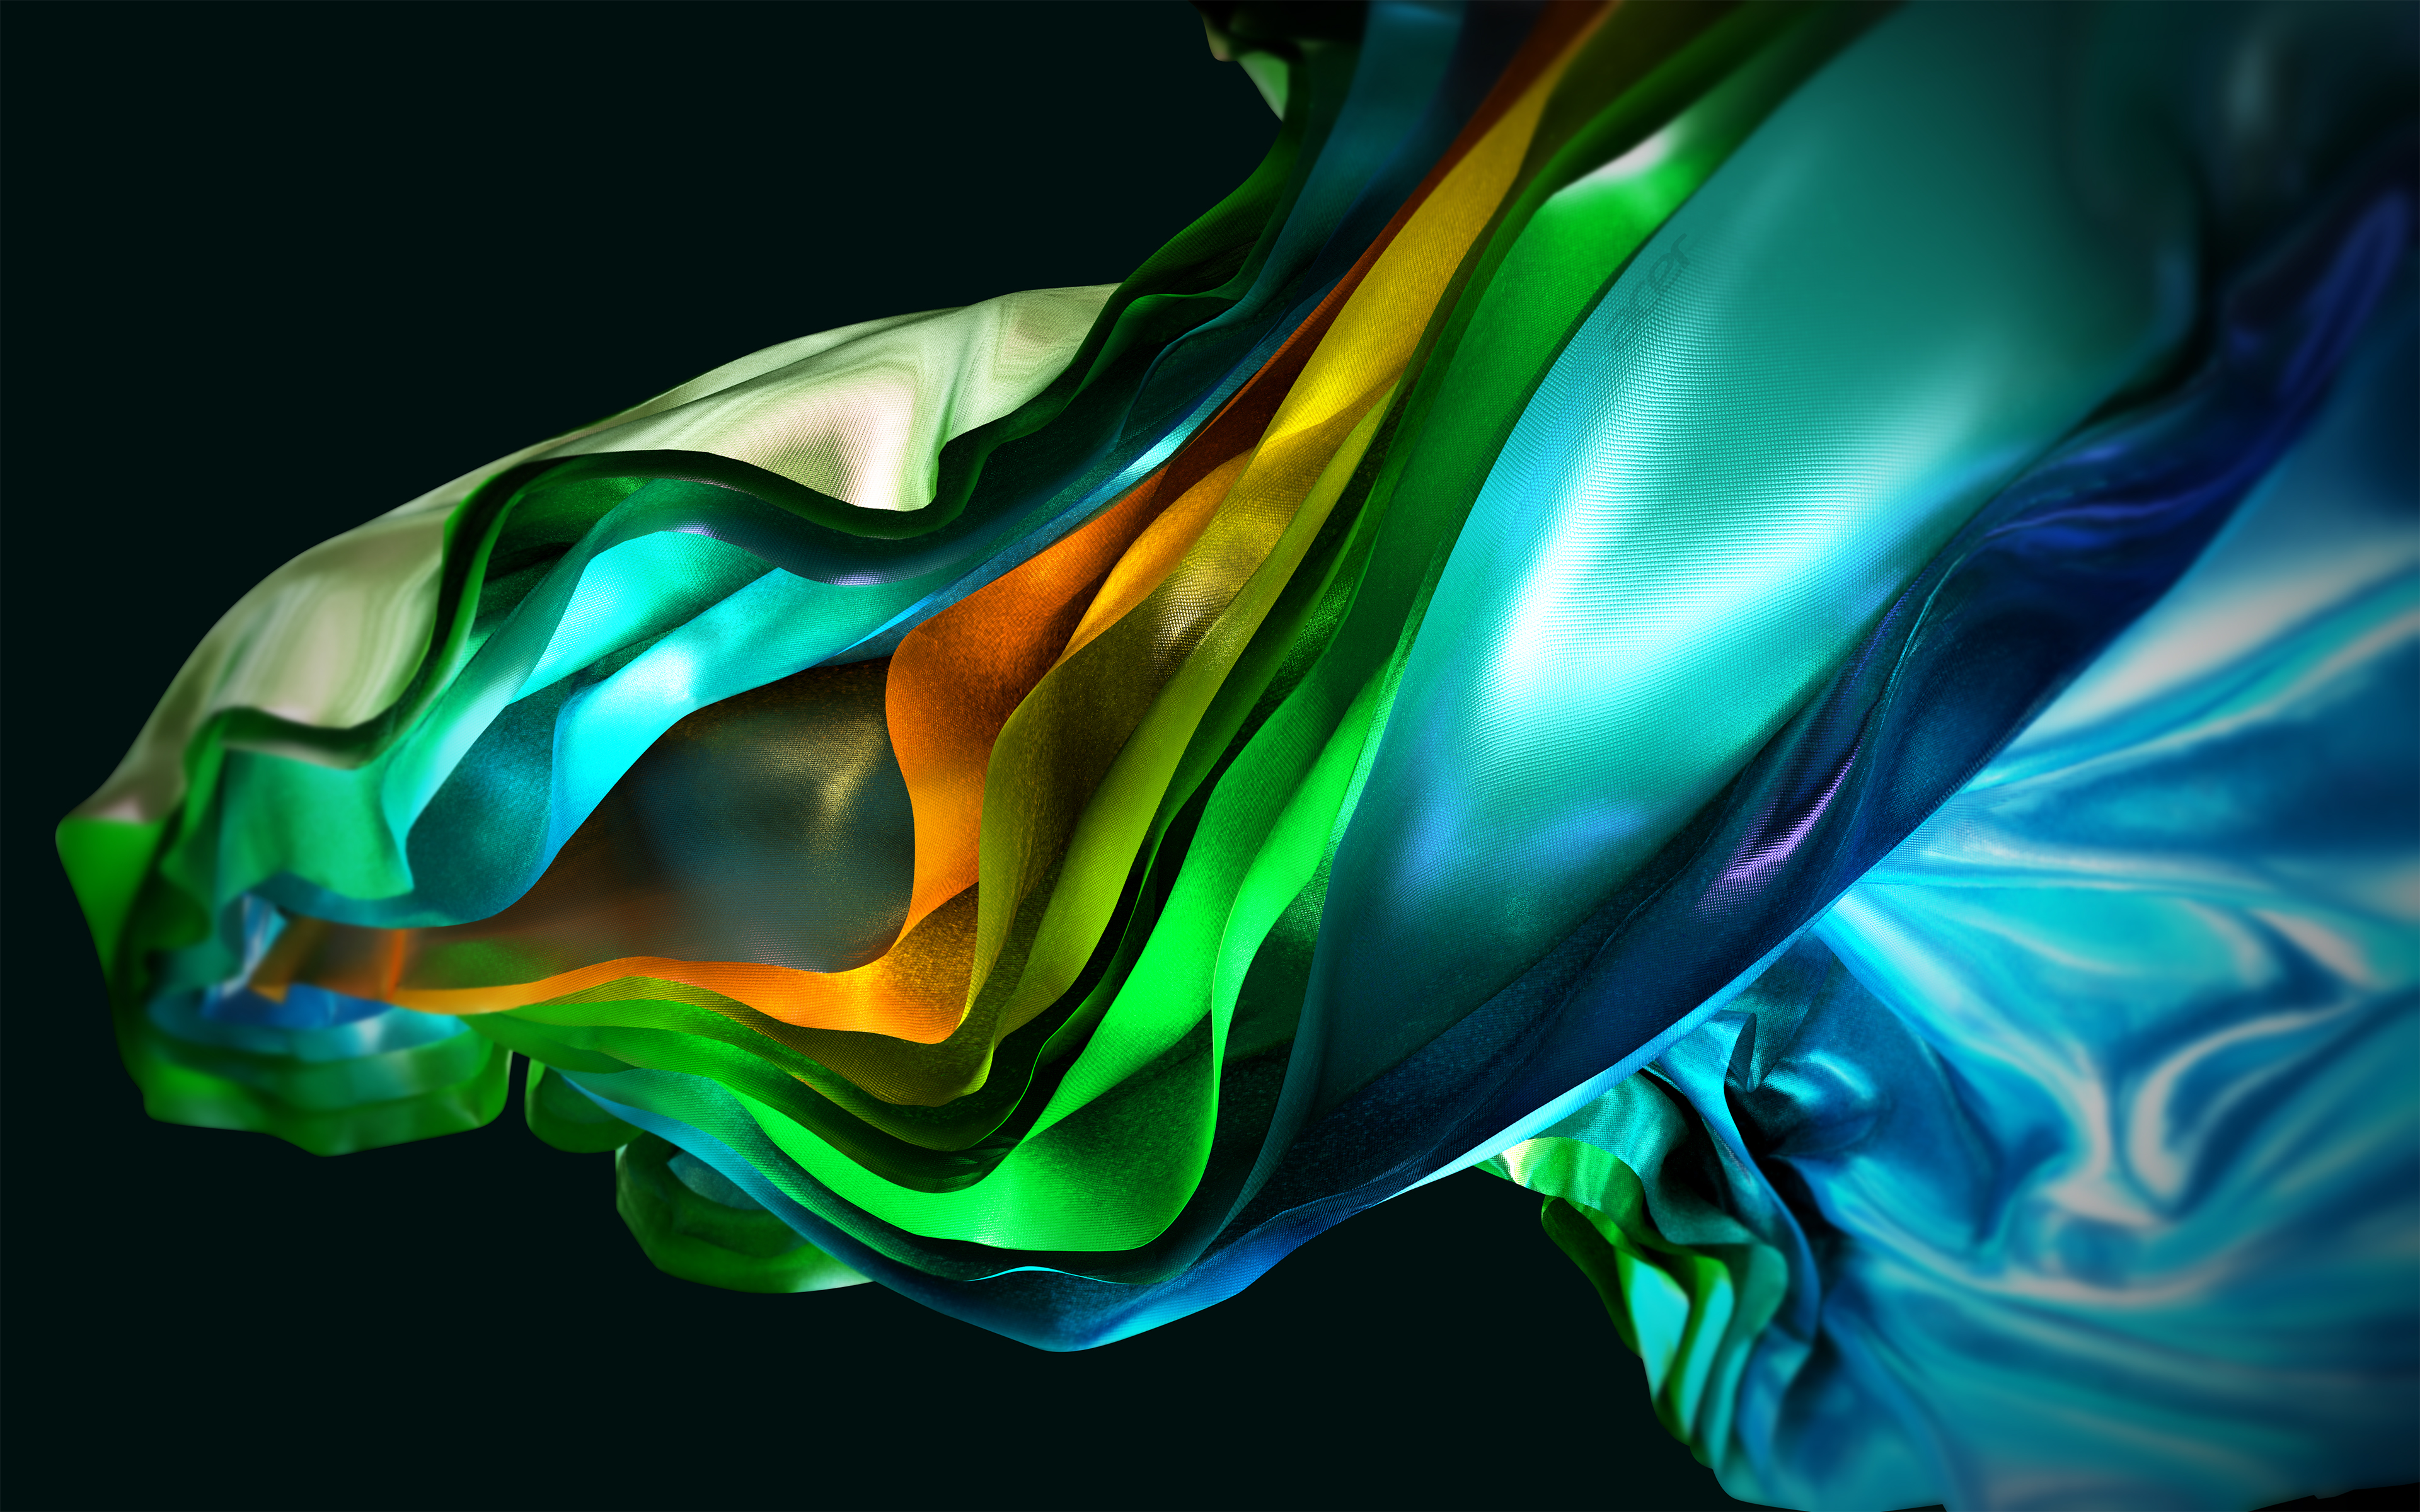
\includegraphics[width=\textwidth]{Bild1.jpg}
        \caption{Bild links}
    \end{minipage}
    \begin{minipage}[t]{0.3\textwidth}
        \centering
        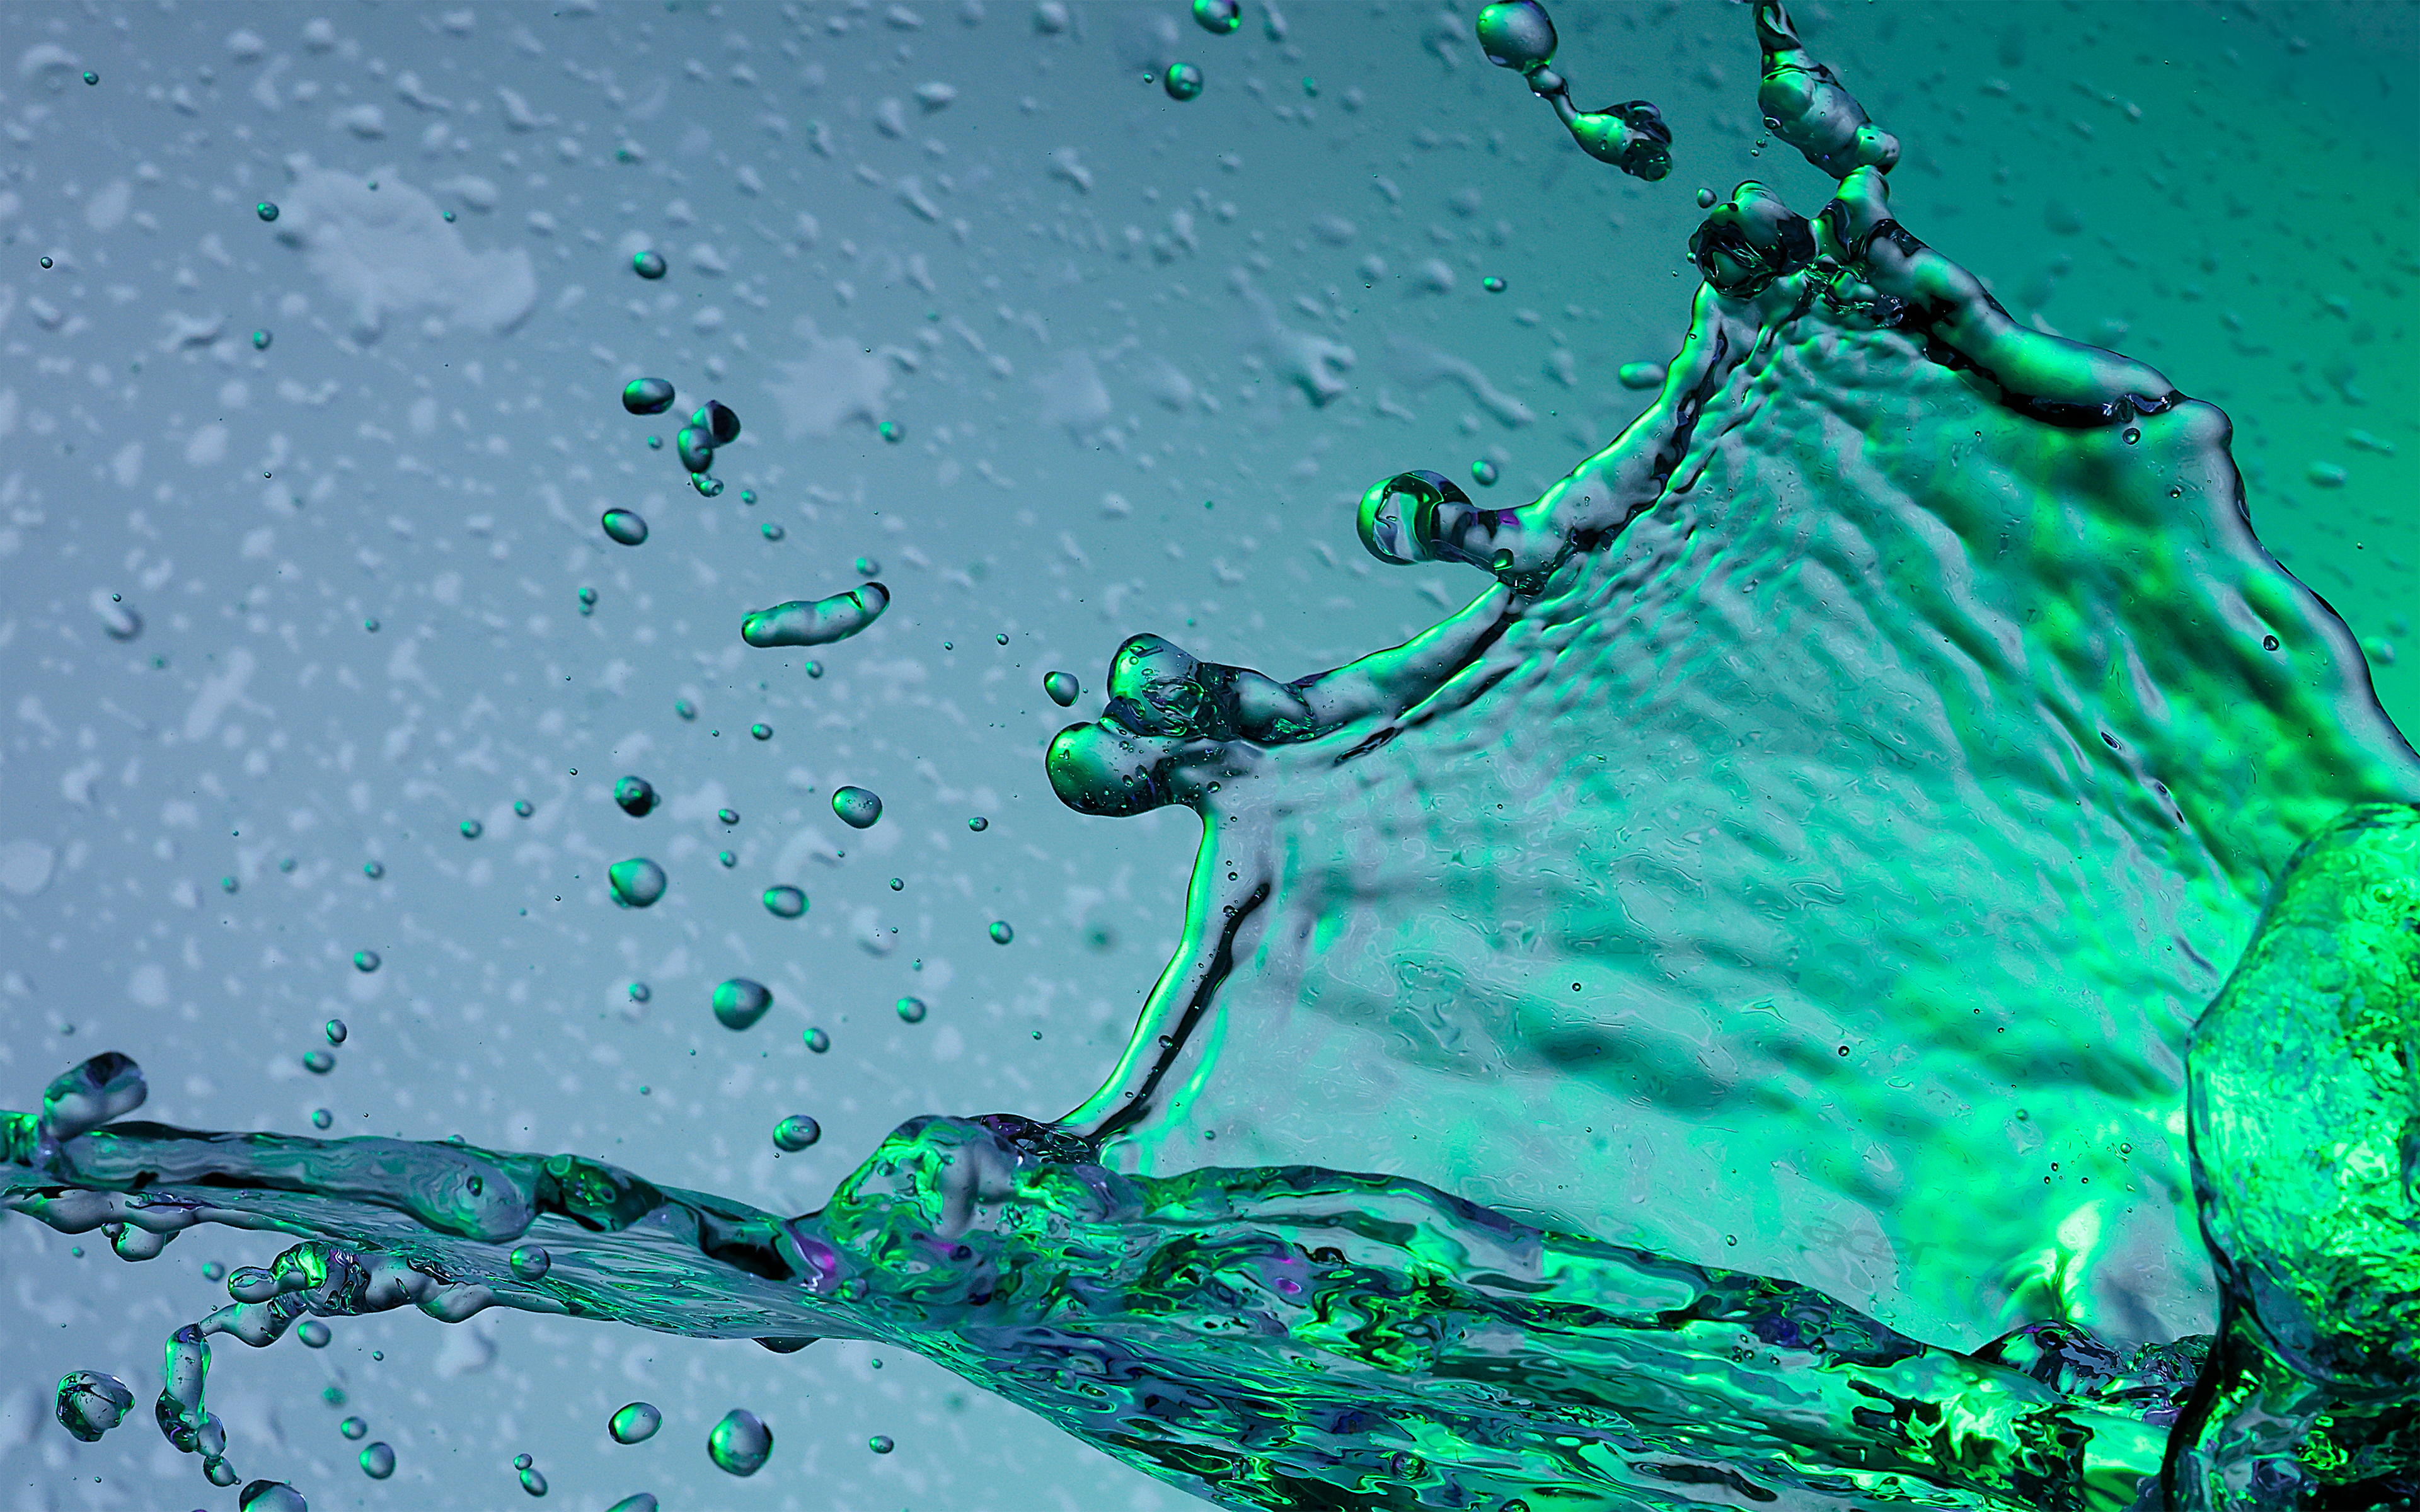
\includegraphics[width=\textwidth]{Bild2.jpg}
        \caption{Bild Mitte}
    \end{minipage}
    \begin{minipage}[t]{0.3\textwidth}
        \centering
        
\includegraphics[width=\textwidth]{Bild3.jpg}
        \caption{Bild rechts}
    \end{minipage}
    \centering
    \caption{Drei Bilder nebeneinander}
\end{figure}

\vspace{0.5 cm}

\begin{figure}[!h]
  \centering

  \begin{minipage}{0.45\textwidth}
    \centering
    \includegraphics[width=\linewidth]{example-image-a}
    \caption{Bild A}
    \label{fig:first}
  \end{minipage}
  \hfill
  \begin{minipage}{0.45\textwidth}
    \centering
    \includegraphics[width=\linewidth]{example-image-b}
    \caption{Bild B}
    \label{fig:second}
  \end{minipage}

  \caption{Zwei Bilder nebeneinander}
  \label{fig:both}
\end{figure}

\newpage

\subsection{Bild und Text nebeneinander}  % Unterabschnitt für Bild-Text-Kombination
\begin{figure}[!h]  % Neue Floating-Umgebung

  \centering  % Zentriert den gesamten Inhalt
  \begin{minipage}[b]{0.45\textwidth}  % Linke Minipage, 45% der Textbreite, am unteren Rand ausgerichtet
    \centering  % Zentriert den Inhalt der Minipage
    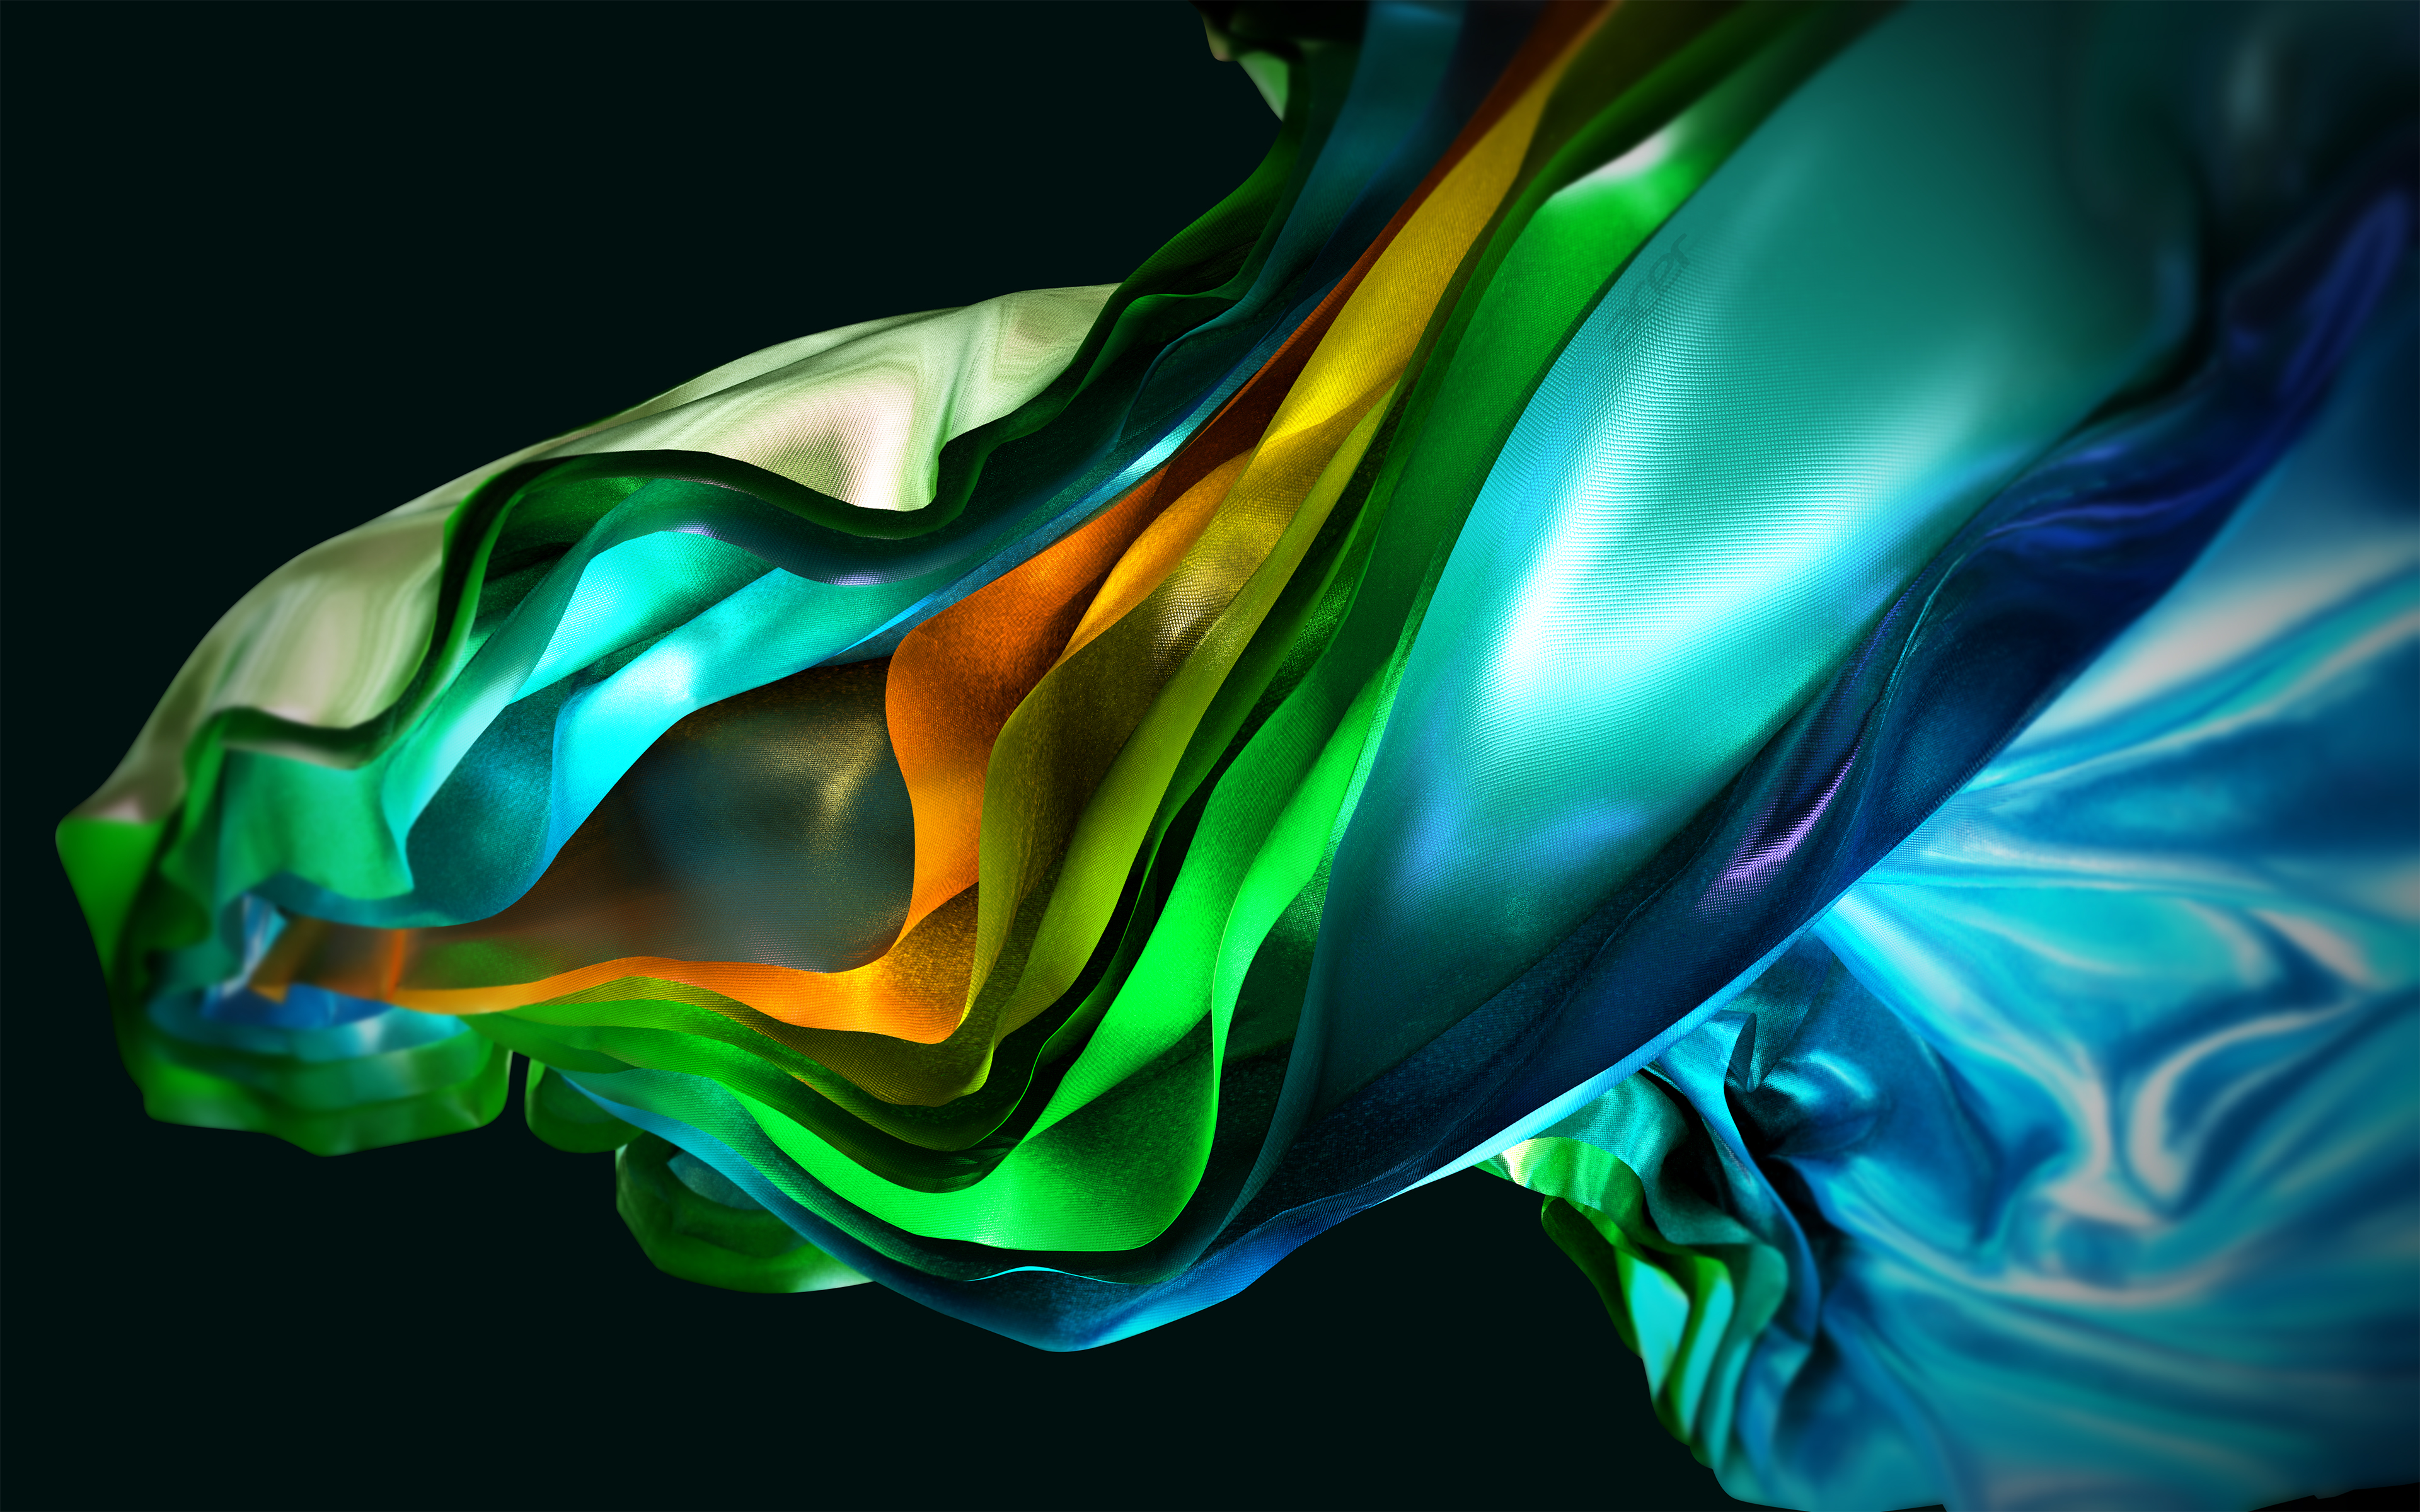
\includegraphics[width=\textwidth]{Bild1.jpg}  % Bild mit voller Breite der Minipage
    \caption{Bild links}  % Bildunterschrift für linke Seite
  \end{minipage}
  \begin{minipage}[b]{0.45\textwidth}  % Rechte Minipage, 45% der Textbreite
    \raggedright  % Text linksbündig ausrichten
    % Beispieltext mit manuellen Zeilenumbrüchen
    Dies ist ein Beispieltext, der rechts neben dem Bild steht.\\
    Er kann mehrere Zeilen umfassen und erklärt das Bild.\\

    \vspace{0.8 cm}  % Vertikaler Abstand von 0.8cm

    In diesem Fall sehen wir ein schönes Laptop Hintergundbild.\\
    \caption{Text rechts}  % Bildunterschrift für rechte Seite
  \end{minipage}
\end{figure}
    
\subsection{Code und Text nebeneinander}  % Unterabschnitt für Code-Text-Kombination
\begin{figure}[!h]  % Neue Floating-Umgebung

  \centering  % Zentriert den gesamten Inhalt
  \begin{minipage}[b]{0.55\textwidth}  % Linke Minipage für Code, 55% der Textbreite
    \centering  % Zentriert den Inhalt der Minipage
    % Code-Block mit definiertem Stil
\begin{lstlisting}[style=cstyle]
#include <stdio.h>

int main(void) {
    printf("Hello, World!\n");
    return 0;
}
\end{lstlisting}
    \caption{Code links}  % Bildunterschrift für den Code
  \end{minipage}
  \begin{minipage}[b]{0.4\textwidth}  % Rechte Minipage für Text, 40% der Textbreite
    \centering  % Zentriert den Inhalt
    \begin{itemize}  % Aufzählungsliste
      \item Dies ist ein einfaches C-Programm.  % Erster Listenpunkt
      \item Es gibt "Hello, World!" auf der Konsole aus.  % Zweiter Listenpunkt
    \end{itemize}
    \caption{Text rechts}  % Bildunterschrift für den Text
  \end{minipage}
\end{figure}



\newpage

% =====================================================================
%Bachleitner
% =====================================================================
\section{Beispiele: Tabellenformate}
{\large von Florian Bachleitner-Huber}

\vspace{1 cm}

In diesem Dokument sind mehrere Möglichkeiten gezeigt, wie man Tabellen mit drei Spalten in LaTeX setzen kann. Zu jeder Tabelle gibt es eine kurze Erklärung.

\subsection*{1) Einfache linksbündige Tabelle}
% Beispiel 1: einfache linksbündige Tabelle
	\textit{Erklärung:} Standardtabular mit drei linksbündigen Spalten (l).	%beschreibt, dass hier eine Standarttabelle mit linksbündigen Spalten gezeigt wird.
\begin{table}[h!]															%erlaubt Latex Tabellen zu positionieren,h! heißt das es hundertprozentig hier erscheinen soll.
	\centering								                                %zentriert die Tabelle auf der Seite
	\caption{Einfache linksbündige Tabelle}                                 %Beschriftung der Tabelle
	\begin{tabular}{lll}                                                    %Tabellenumgebung mit 3 linken Spalten
	
		Spalte 1 & Spalte 2 & Spalte 3 \\                                   %Tabellenkopf
		\midrule                                                            %horizontale Linie
		A1 & A2 & A3 \\                                                     %erste Datenzeile
		B1 & B2 & B3 \\                                                     %zweite Datenzeile
		\bottomrule                                                         %horizontale Linie unten
	\end{tabular}                                                           %Ende der Tabellenumgebung
\end{table}                                                                 %Ende der Tabelle

\subsection*{2) Zentrierte und rechtsbündige Spalten}
% Beispiel 2: zentrierte und rechtsbündige Spalten
	\textit{Erklärung:} Verwende c für zentriert und r für rechtsbündig.
\begin{table}[h!]
	\centering
	\caption{Zentriert / Rechts}
	\begin{tabular}{crr}
	
		Spalte 1 & Spalte 2 & Spalte 3 \\
		\midrule
		Text & 123 & 4.56 \\
		Mehr & 78 & 9.10 \\
		\bottomrule
	\end{tabular}
\end{table}

\subsection*{3) Vertikale Linien}
% Beispiel 3: vertikale Linien in der Tabelle
	\textit{Erklärung:} Senkrechte Linien mit |; oft weniger empfohlen, aber in manchen Fällen gebraucht.
\begin{table}[h!]
	\centering
	\caption{Mit vertikalen Linien}
	\begin{tabular}{|l|c|r|}
		\hline
		Spalte 1 & Spalte 2 & Spalte 3 \\
		\hline
		A & B & C \\
		D & E & F \\
		\hline
	\end{tabular}
\end{table}

\subsection*{4) Feste Spaltenbreite mit p{width}}
% Beispiel 4: feste Spaltenbreite mit p{..}
	\textit{Erklärung:} p{<Breite>} erlaubt Textumbruch in Zellen.
\begin{table}[h!]
	\centering
	\caption{Feste Breite (p{4cm})}
	\begin{tabular}{p{4cm}p{4cm}p{4cm}}

		 Überschrift 1 &  Überschrift 2 &  Überschrift 3 \\
		\midrule
		Dies ist ein längerer Text, der umbrechen soll. & Kurz & Noch ein langer Text, der umbrechen wird. \\
		\bottomrule
	\end{tabular}
\end{table}

\subsection*{5) Flexible Breite mit tabularx}
% Beispiel 5: flexible Breite mit tabularx
	\textit{Erklärung:} \texttt{tabularx} mit X-Spalten verteilt die Breite automatisch.
\begin{table}[h!]
	\centering
	\caption{tabularx mit X-Spalten}
	\begin{tabularx}{\textwidth}{X X X}
		
		Überschrift 1 & Überschrift 2 & Überschrift 3 \\
		\midrule
		Text links & Mittel & Rechts \\
		Noch Text & Noch mehr & Und noch mehr \\
		\bottomrule
	\end{tabularx}
\end{table}

\subsection*{6) Tabellen mit booktabs}
% Beispiel 6: booktabs für saubere Linien
	\textit{Erklärung:} \texttt{booktabs} erzeugt professionellere horizontale Linien (toprule, midrule, bottomrule).
\begin{table}[h!]
	\centering
	\caption{booktabs Beispiel}
	\begin{tabular}{lll}
		
		Spalte A & Spalte B & Spalte C \\
		\midrule
		1 & 2 & 3 \\
		4 & 5 & 6 \\
		\bottomrule
	\end{tabular}
\end{table}

\newpage

\subsection*{7) Zahlen und Einheiten mit siunitx}
% Beispiel 7: Zahlenformatierung mit siunitx
	\textit{Erklärung:} \texttt{siunitx} formatiert Zahlen und Einheiten sauber; r-Alignment mit S-Spalten.
\begin{table}[h!]
	\centering
	\caption{siunitx Beispiel}
	\begin{tabular}{l S S}
	
		Messung & {Wert 1} & {Wert 2} \\
		\midrule
		Probe A & 1234.56 & 7.89 \\
		Probe B & 12.3 & 456.0 \\
		\bottomrule
	\end{tabular}
\end{table}

\subsection*{8) Mehrere Zeilen }
% Beispiel 8: multirow / multicolumn
	\textit{Erklärung:} \texttt{multirow} und \texttt{multicolumn} erlauben das Zusammenführen von Zellen.
	\begin{table}[h!]
	\centering
	\caption{multirow / multicolumn}
	\begin{tabular}{lll}
			\toprule
		& Spalte 2 & Spalte 3 \\
		\midrule
		\multirow{2}{*}{Gruppe 1} & A & B \\
		 & C & D \\
		\midrule
		\multicolumn{2}{c}{Zusammengefasst} & E \\
		\bottomrule
	\end{tabular}
\end{table}

\subsection*{9) Lange Tabellen über Seiten: longtable}
% Beispiel 9: longtable für mehre Seiten
	\textit{Erklärung:} \texttt{longtable} erlaubt Tabellen, die sich über mehrere Seiten erstrecken.
\begin{longtable}{lll}
	\caption{longtable Beispiel} \\
	\toprule
	Kopf 1 & Kopf 2 & Kopf 3 \\
	\midrule
	\endfirsthead
	\multicolumn{3}{c}{Fortsetzung von vorheriger Seite} \\
	\toprule
	Kopf 1 & Kopf 2 & Kopf 3 \\
	\midrule
	\endhead
	Ein & Zwei & Drei \\
	Eins & Zwei & Drei \\
	% (weitere Zeilen würden hier folgen)
	\bottomrule
\end{longtable}

\subsection*{10) Technische Tabelle}
\begin{center}
\renewcommand{\arraystretch}{1}
\begin{tabular}{c|c}

\textbf{Gerät} & \textbf{Nr. /Wert} \\
\hline
Tektronix TBS      & SN: C024671 \\
Fluke 175          & SN: 35950210 \\
Conrad Steckb.     & Nr.\ 52\,69\,23 \\
OPAMP TL084        & n/A \\
Widerstand         & 1{,}2 k$\Omega$ \\
Widerstand         & 2{,}2 k$\Omega$ \\
Widerstand         & 10 k$\Omega$ \\
Widerstand         & 39 k$\Omega$ \\
Widerstand         & 68 k$\Omega$ \\
Poti               & 100 k$\Omega$ \\
Kondensator        & 10 nF \\

\end{tabular}
\end{center}


\newpage
% =====================================================================
%Schönauer
% =====================================================================
\section{Abbildungen in LaTeX}
{\large von Simon Schönauer}

\vspace{1 cm}

\large Vollständige Referenz mit allen Szenarien
% =====================================================================
\subsection{Grundlagen und einfache Abbildungen}
% =====================================================================

\subsubsection{Einfache Abbildung mit verschiedenen Positionierungen}

\paragraph{Positionierung mit [H] (exakt hier)}
\begin{figure}[H]
  % [H] = Abbildung wird GENAU hier platziert (nicht verschieben!)
  % Benötigt das float-Paket
  \centering
  % Bild horizontal zentrieren
  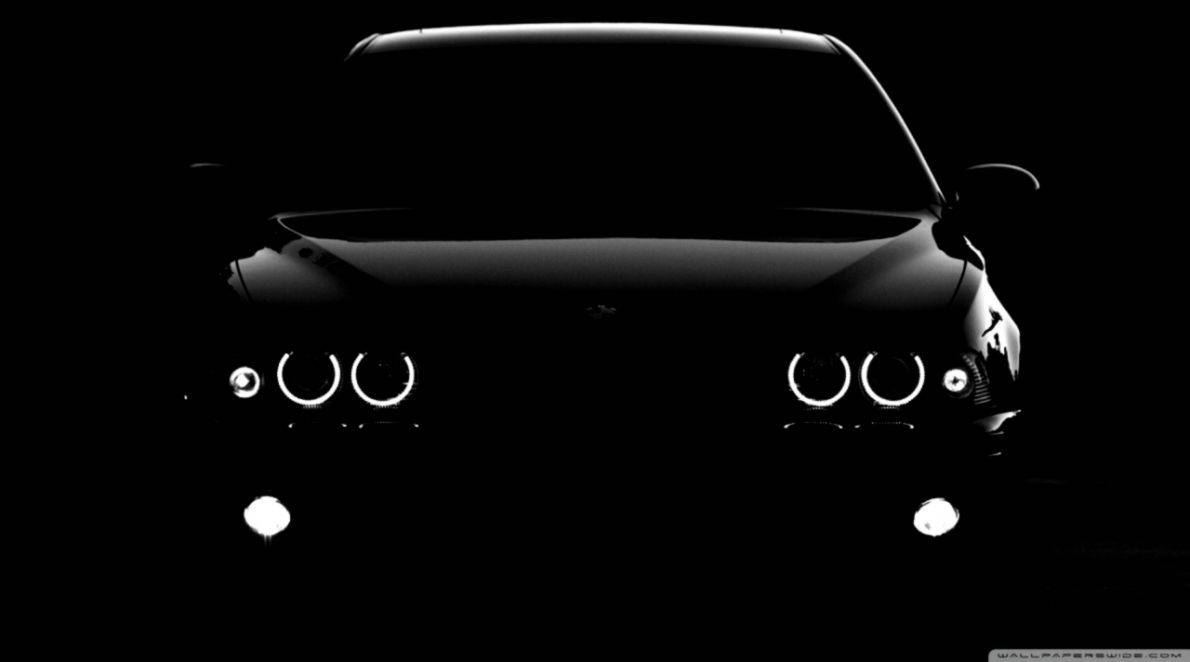
\includegraphics[width=0.6\textwidth]{BMW.jpg}
  % width=0.6\textwidth bedeutet: Breite = 60% der Textbreite
  \caption{Abbildung mit [H] wird genau hier platziert.}
  % Bildunterschrift unter dem Bild
  \label{fig:einfach-h}
  % Label für Referenzierung im Text (mit \ref{fig:einfach-h})
\end{figure}

\paragraph{Positionierung mit [htbp] (LaTeX entscheidet)}
\begin{figure}[htbp]
  % [htbp] = LaTeX entscheidet selbst die beste Position
  % h = here (hier bevorzugt)
  % t = top (oben auf der Seite)
  % b = bottom (unten auf der Seite)  
  % p = page (eigene Seite nur für Abbildungen)
  \centering
  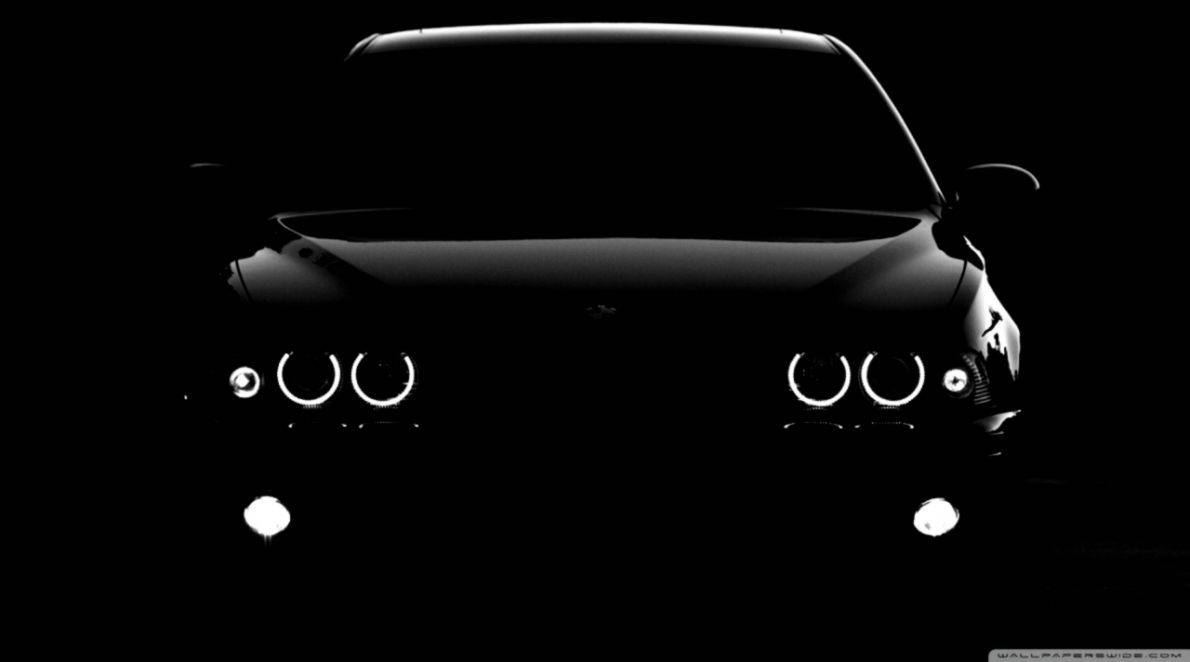
\includegraphics[width=0.6\textwidth]{BMW.jpg}
  \caption{Abbildung mit [htbp] wird von LaTeX optimal platziert.}
  \label{fig:einfach-htbp}
\end{figure}

\subsubsection{Referenzierung im Text}
% Mit \ref{label} wird die Abbildungsnummer eingefügt
% Mit \pageref{label} wird die Seitenzahl eingefügt
% ~ erzeugt ein geschütztes Leerzeichen (verhindert Zeilenumbruch)
Wie in Abbildung~\ref{fig:einfach-h} auf Seite~\pageref{fig:einfach-h} zu sehen ist, lassen sich Bilder leicht einfügen. Man kann auch auf Abbildung~\ref{fig:einfach-htbp} verweisen.

% =====================================================================
\subsection{Größenanpassung und Skalierung}
% Es gibt drei Hauptmethoden: width, height und scale
% =====================================================================

\subsubsection{Breitenanpassung}
\begin{figure}[H]
  \centering
  % Zwei Bilder nebeneinander mit unterschiedlicher Breite
  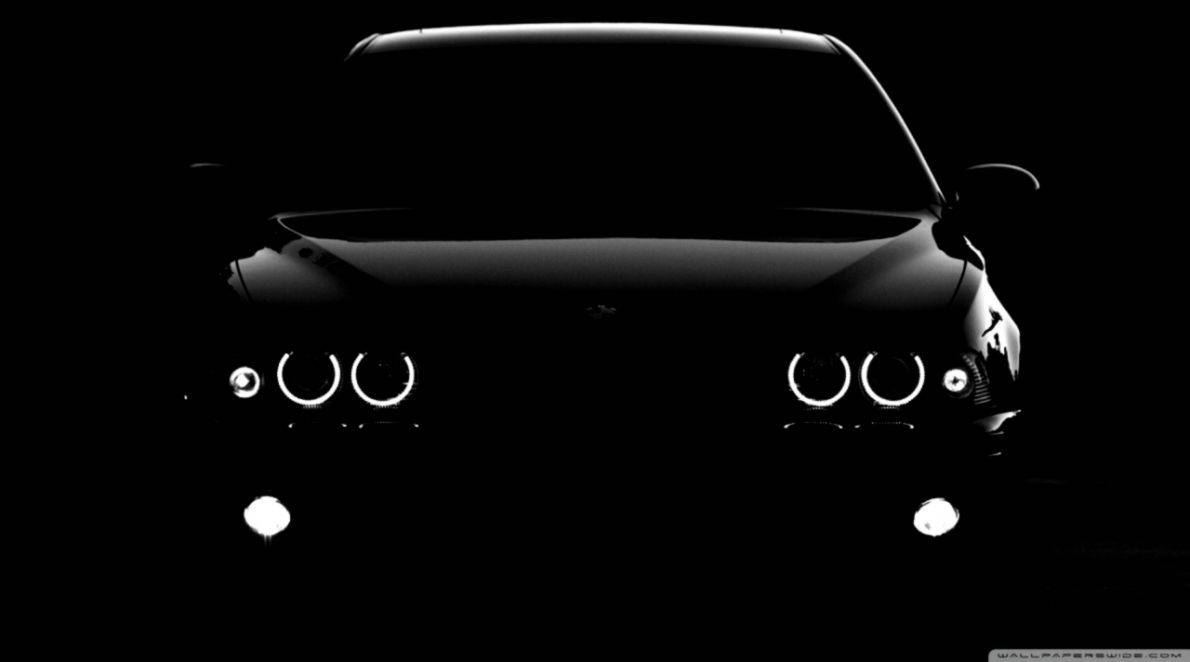
\includegraphics[width=0.4\textwidth]{BMW.jpg}
  \hspace{0.05\textwidth}
  % \hspace = horizontaler Abstand zwischen den Bildern (5% der Textbreite)
  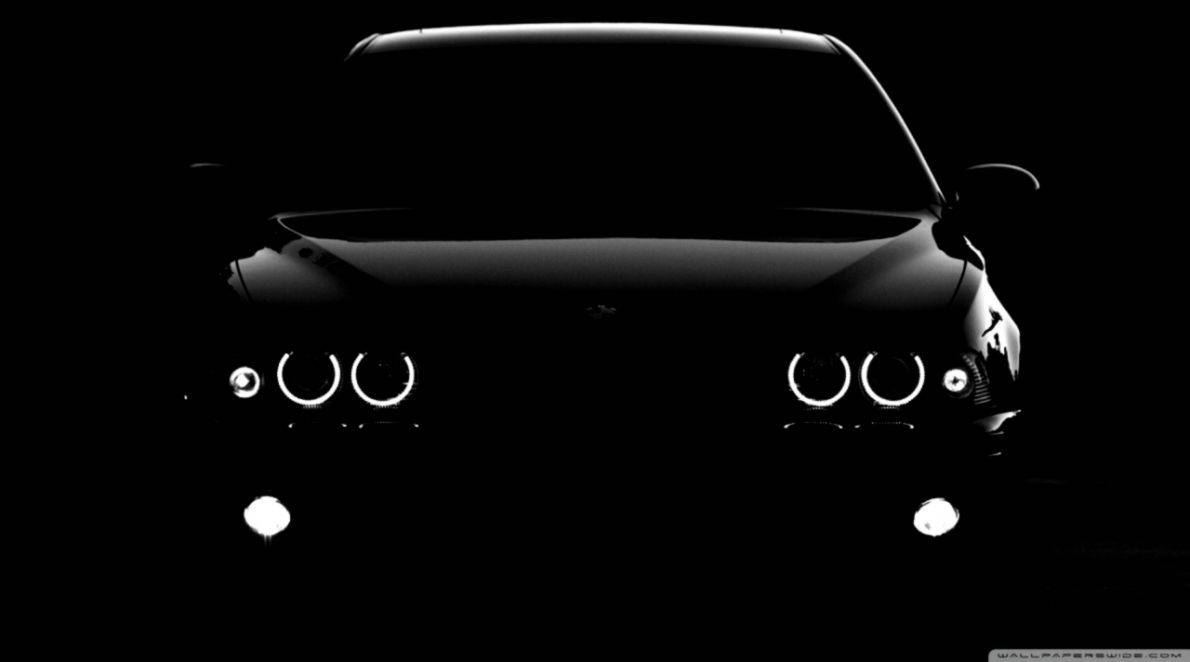
\includegraphics[width=0.5\textwidth]{BMW.jpg}
  \caption{Links: 40\% Textbreite, Rechts: 50\% Textbreite.}
  \label{fig:breite}
\end{figure}

\subsubsection{Höhenanpassung}
\begin{figure}[H]
  \centering
  % Bei height wird die Breite automatisch proportional angepasst
  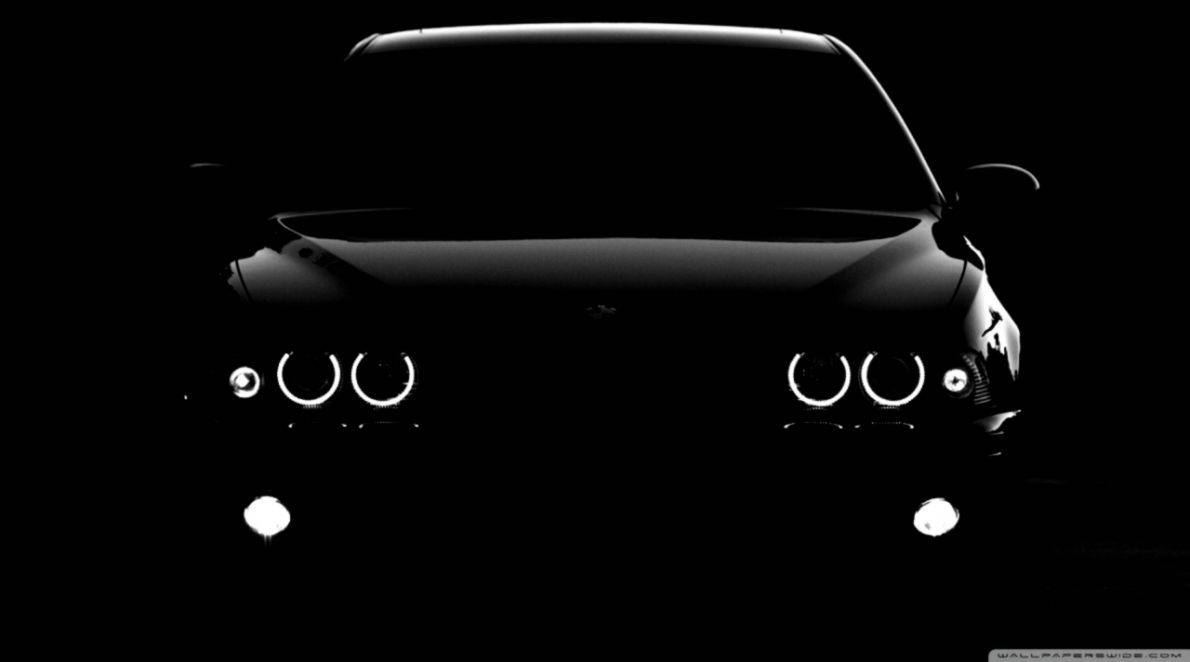
\includegraphics[height=4cm]{BMW.jpg}
  \hspace{1cm}
  % Fester Abstand von 1 cm zwischen den Bildern
  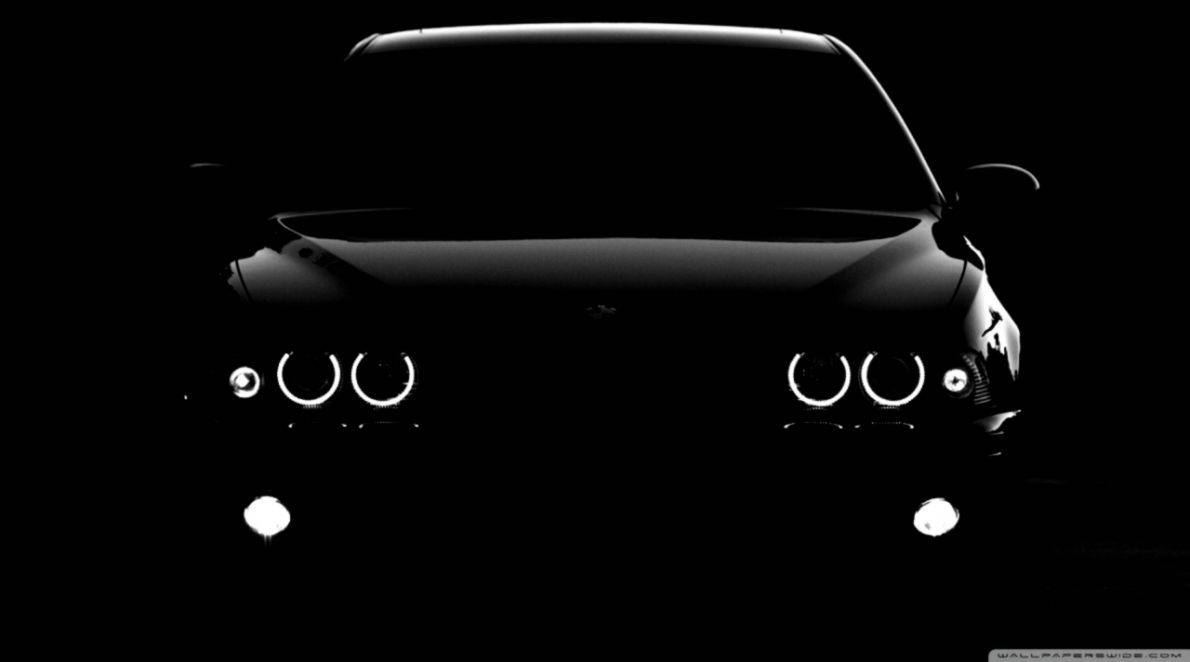
\includegraphics[height=6cm]{BMW.jpg}
  \caption{Links: 4 cm Höhe, Rechts: 6 cm Höhe.}
\end{figure}

\subsubsection{Prozentuale Skalierung}
\begin{figure}[H]
  \centering
  % scale skaliert das Bild basierend auf der Originalgröße
  % scale=0.5 bedeutet 50% der Originalgröße
  % ACHTUNG: scale ignoriert Textbreite!
  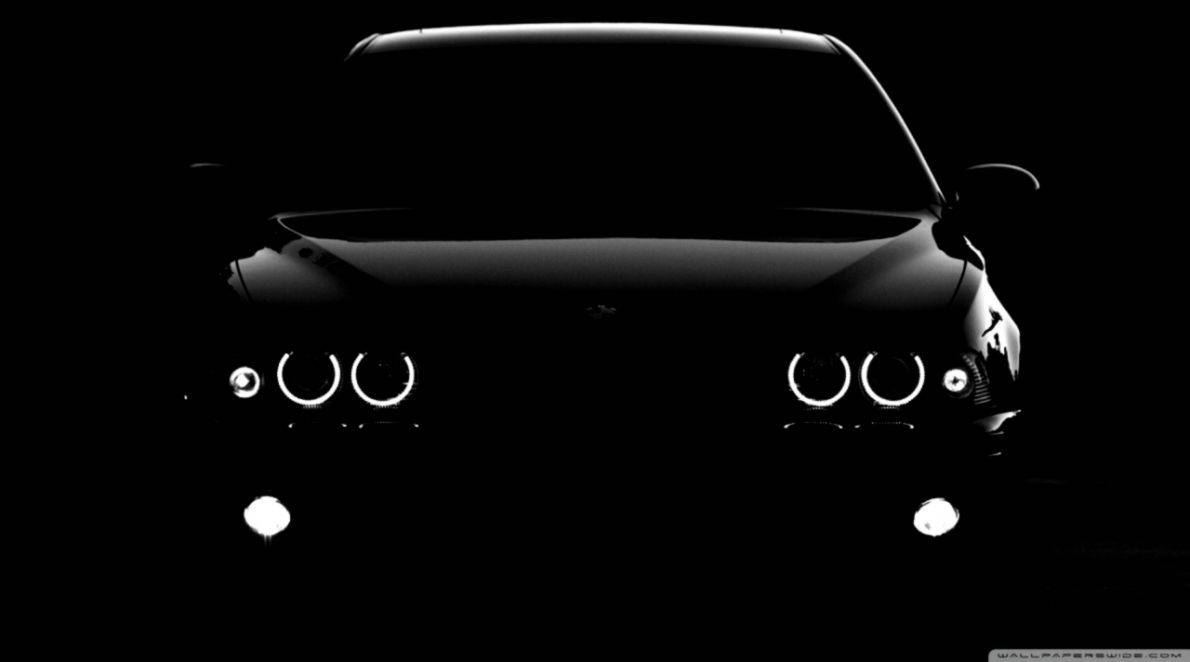
\includegraphics[scale=0.5]{BMW.jpg}
  \caption{Skalierung auf 50\% der Originalgröße.}
\end{figure}

\subsubsection{Breite UND Höhe mit Seitenverhältnis}
\begin{figure}[H]
  \centering
  % keepaspectratio stellt sicher, dass das Bild nicht verzerrt wird
  % Es wird die kleinere der beiden Angaben verwendet
  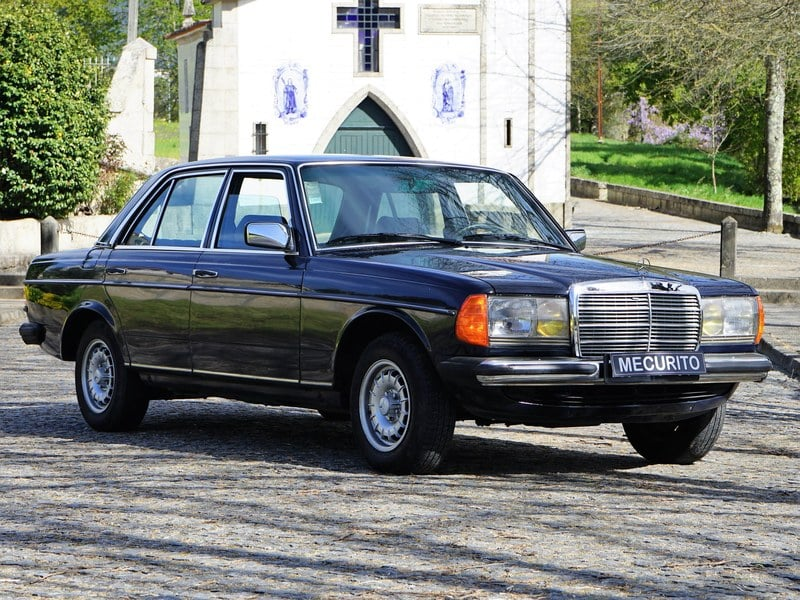
\includegraphics[width=0.8\textwidth,height=8cm,keepaspectratio]{Mercedes.jpg}
  \caption{Maximale Breite 80\% und Höhe 8 cm, Seitenverhältnis erhalten.}
\end{figure}

% =====================================================================
\subsection{Unterabbildungen (Subfigures)}
% Ermöglicht mehrere Bilder in einer Figure-Umgebung
% Benötigt das subcaption-Paket
% =====================================================================

\subsubsection{Zwei Abbildungen nebeneinander}
\begin{figure}[H]
  \centering
  % Erste Unterabbildung (Subfigure)
  \begin{subfigure}[b]{0.45\textwidth}
    % [b] = bottom-aligned (unten ausgerichtet)
    % Alternativen: [t] = top, [c] = center
    % 0.45\textwidth = 45% der Textbreite
    \centering
    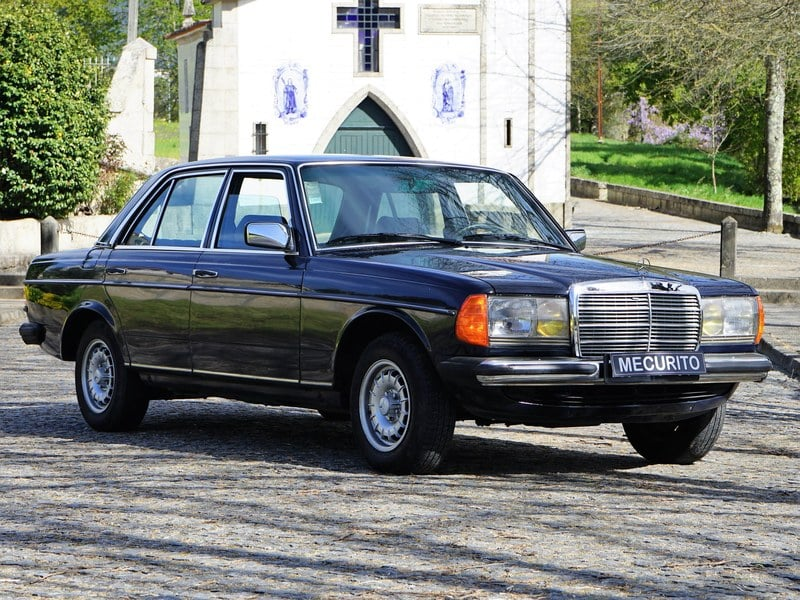
\includegraphics[width=\textwidth]{Mercedes.jpg}
    % \textwidth bezieht sich hier auf die Subfigure-Breite (45%)
    \caption{Mercedes-Benz}
    % Separate Bildunterschrift für diese Subfigure
    \label{fig:sub-mercedes}
    % Eigenes Label für Referenzierung
  \end{subfigure}
  \hfill
  % \hfill = maximaler horizontaler Abstand (verteilt Bilder gleichmäßig)
  % Alternative: \hspace{1cm} für festen Abstand
  \begin{subfigure}[b]{0.45\textwidth}
    \centering
    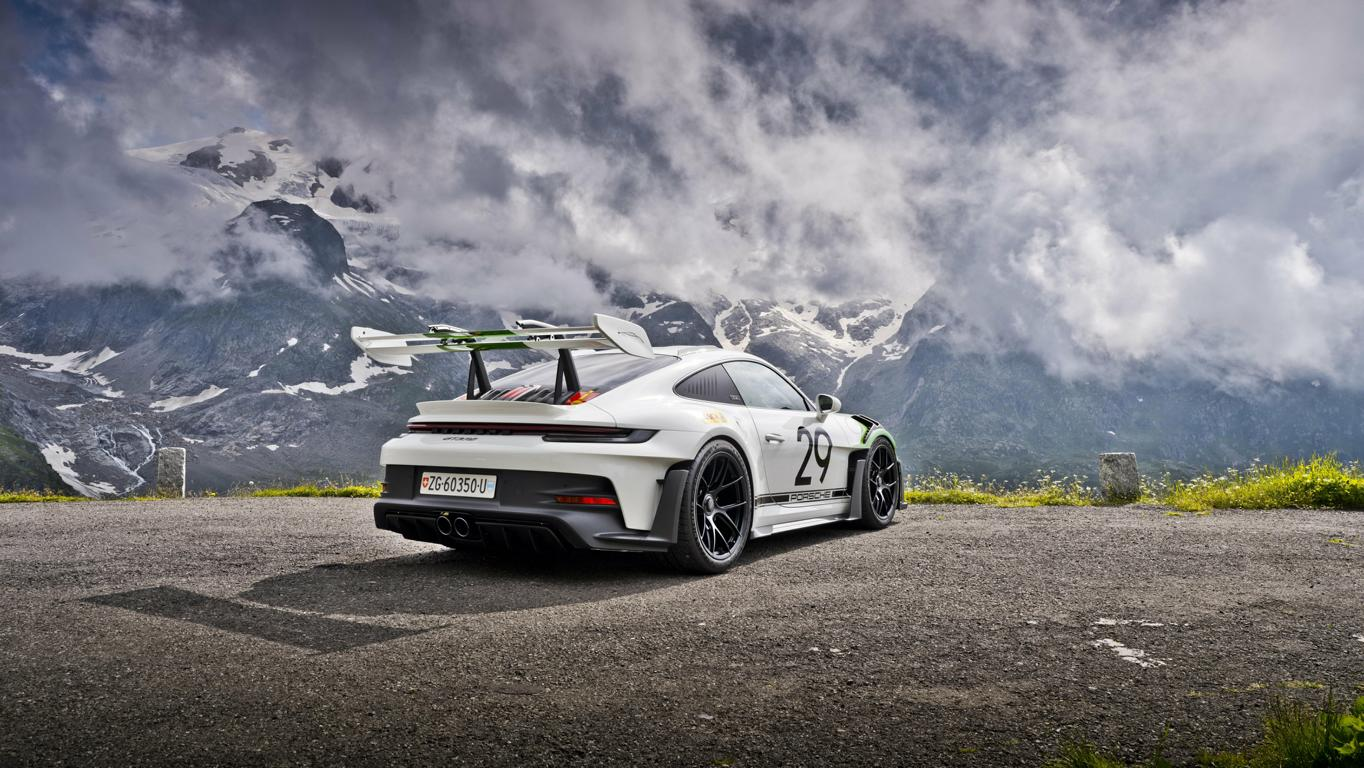
\includegraphics[width=\textwidth]{Porsche.jpg}
    \caption{Porsche}
    \label{fig:sub-porsche}
  \end{subfigure}
  \caption{Zwei Unterabbildungen nebeneinander.}
  % Gemeinsame Hauptbildunterschrift für beide Subfigures
  \label{fig:zwei-neben}
  % Hauptlabel für die gesamte Figure
\end{figure}

\subsubsection{Drei Abbildungen in einer Reihe}
\begin{figure}[H]
  \centering
  % Drei Subfigures mit je 30% Breite (3×30% + Abstände = ~100%)
  \begin{subfigure}[b]{0.3\textwidth}
    \centering
    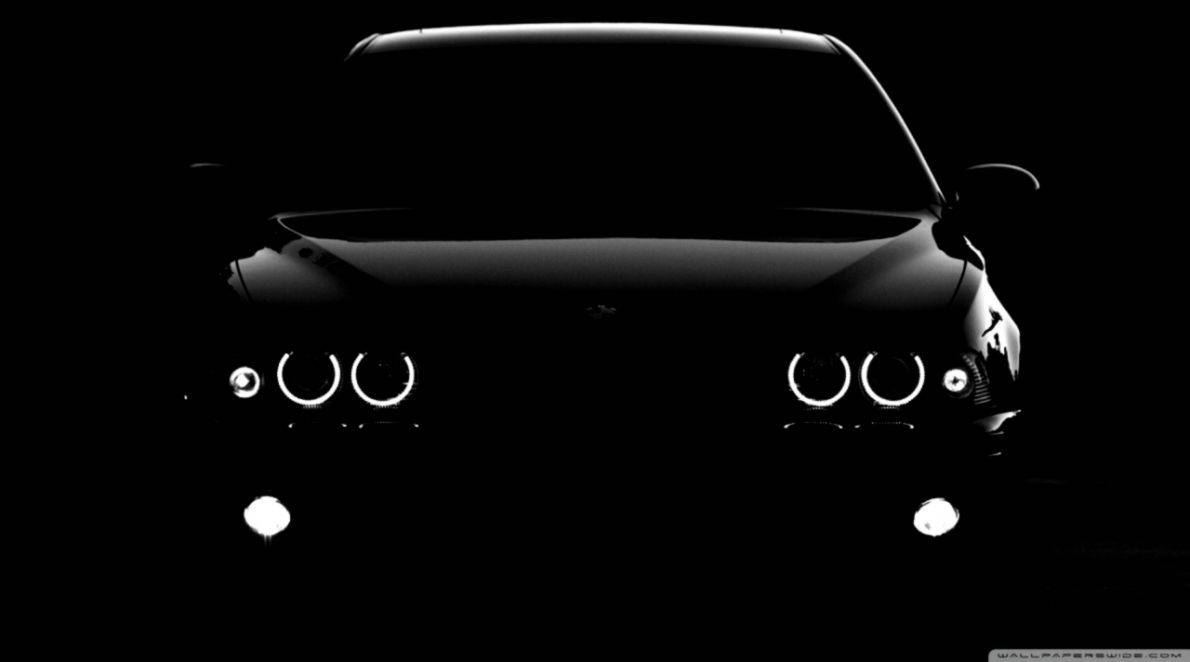
\includegraphics[width=\textwidth]{BMW.jpg}
    \caption{BMW}
  \end{subfigure}
  \hfill
  % \hfill zwischen allen drei Bildern verteilt sie gleichmäßig
  \begin{subfigure}[b]{0.3\textwidth}
    \centering
    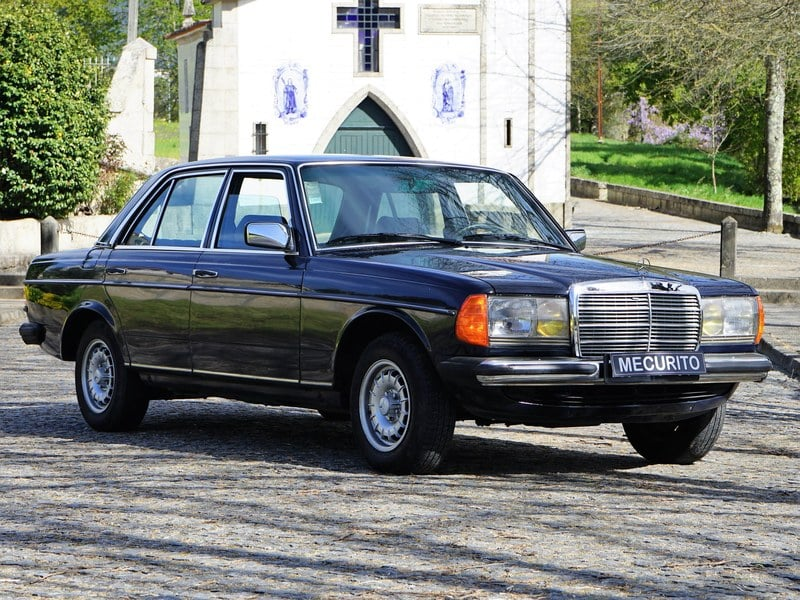
\includegraphics[width=\textwidth]{Mercedes.jpg}
    \caption{Mercedes}
  \end{subfigure}
  \hfill
  \begin{subfigure}[b]{0.3\textwidth}
    \centering
    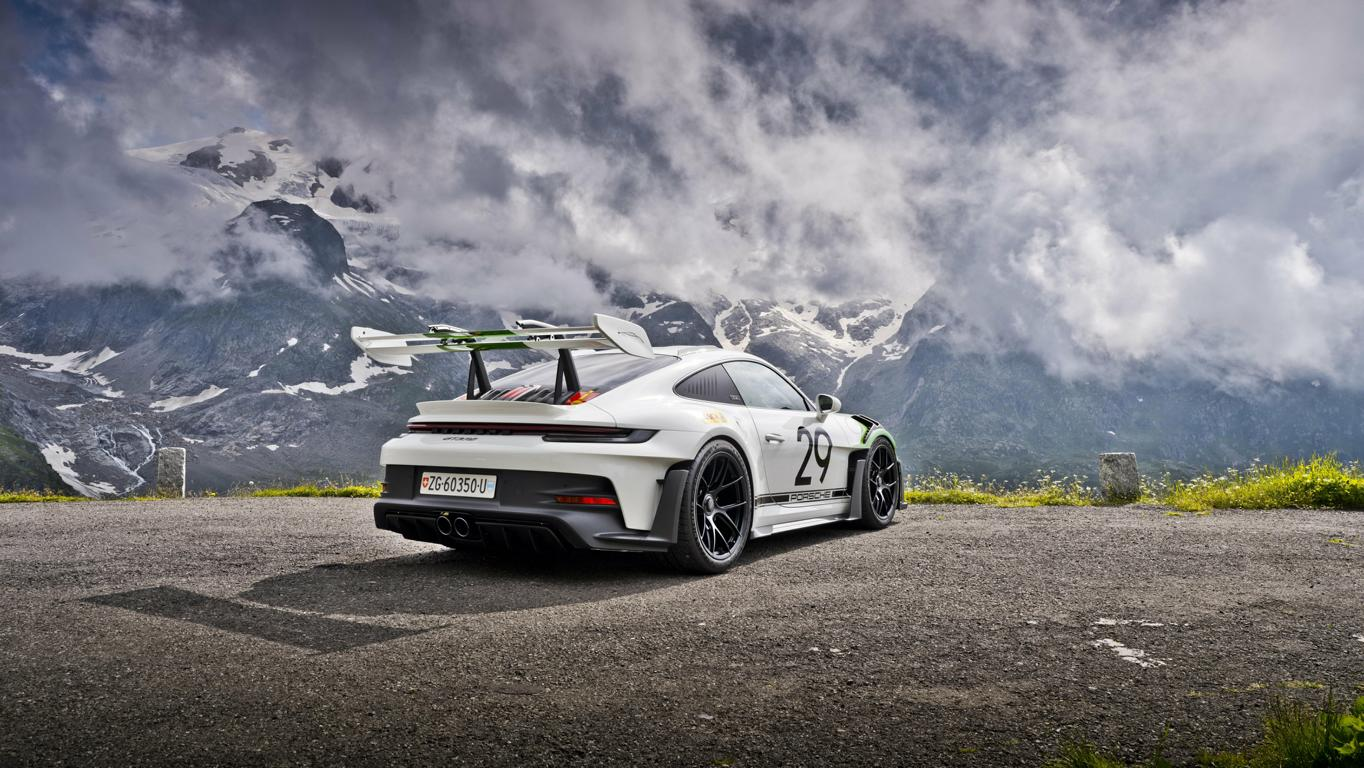
\includegraphics[width=\textwidth]{Porsche.jpg}
    \caption{Porsche}
  \end{subfigure}
  \caption{Drei Unterabbildungen in einer Reihe.}
\end{figure}

\subsubsection{Grid-Layout: 2×2 Unterabbildungen}
\begin{figure}[H]
  \centering
  % Erste Reihe: zwei Subfigures
  \begin{subfigure}[b]{0.45\textwidth}
    \centering
    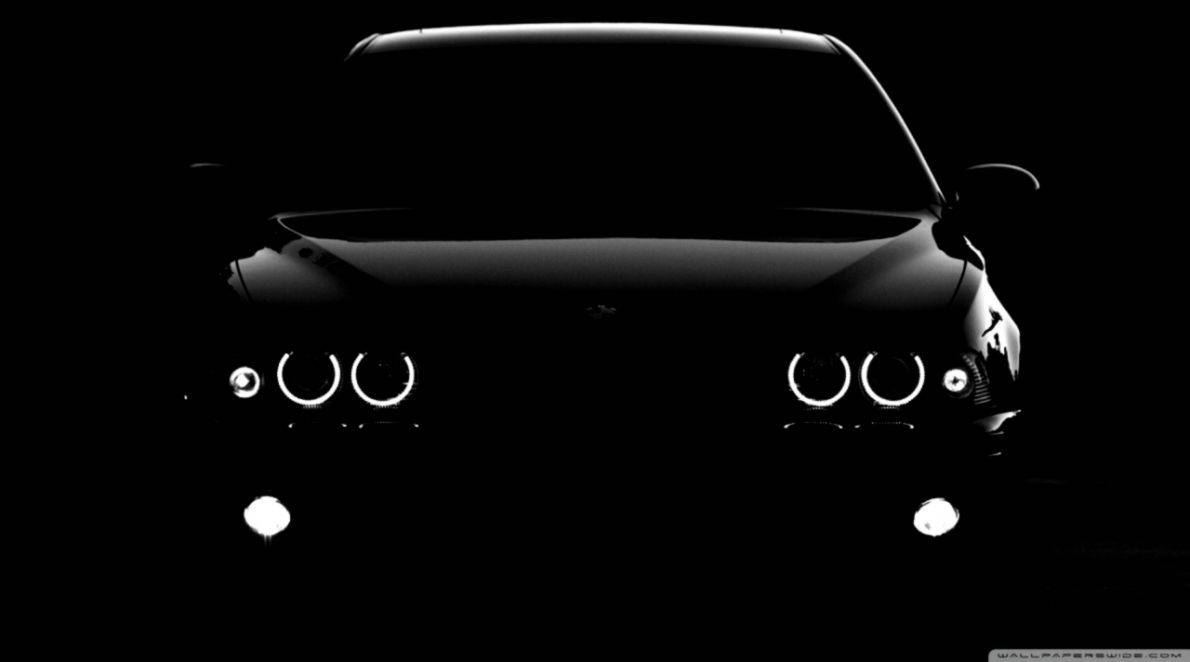
\includegraphics[width=\textwidth]{BMW.jpg}
    \caption{Oben links}
  \end{subfigure}
  \hfill
  \begin{subfigure}[b]{0.45\textwidth}
    \centering
    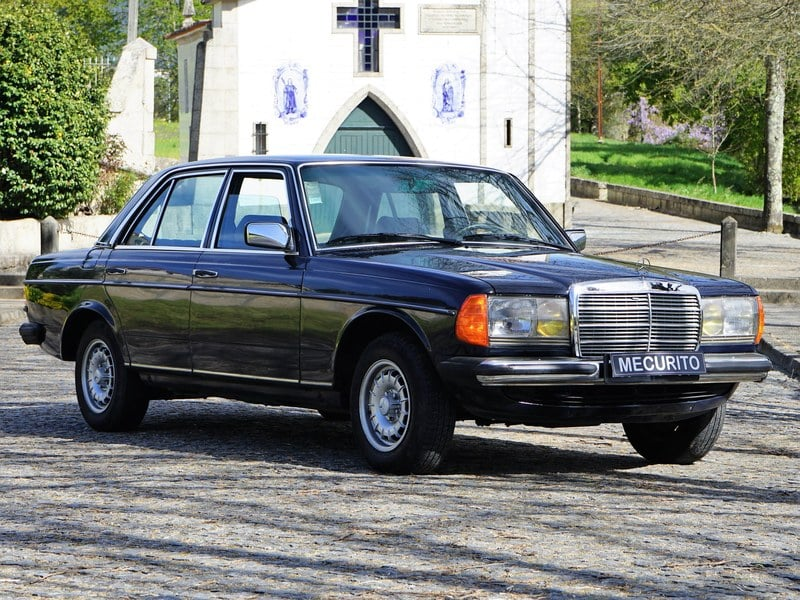
\includegraphics[width=\textwidth]{Mercedes.jpg}
    \caption{Oben rechts}
  \end{subfigure}
  
  \vspace{0.5cm}
  % Vertikaler Abstand zwischen den beiden Reihen
  
  % Zweite Reihe: zwei weitere Subfigures
  \begin{subfigure}[b]{0.45\textwidth}
    \centering
    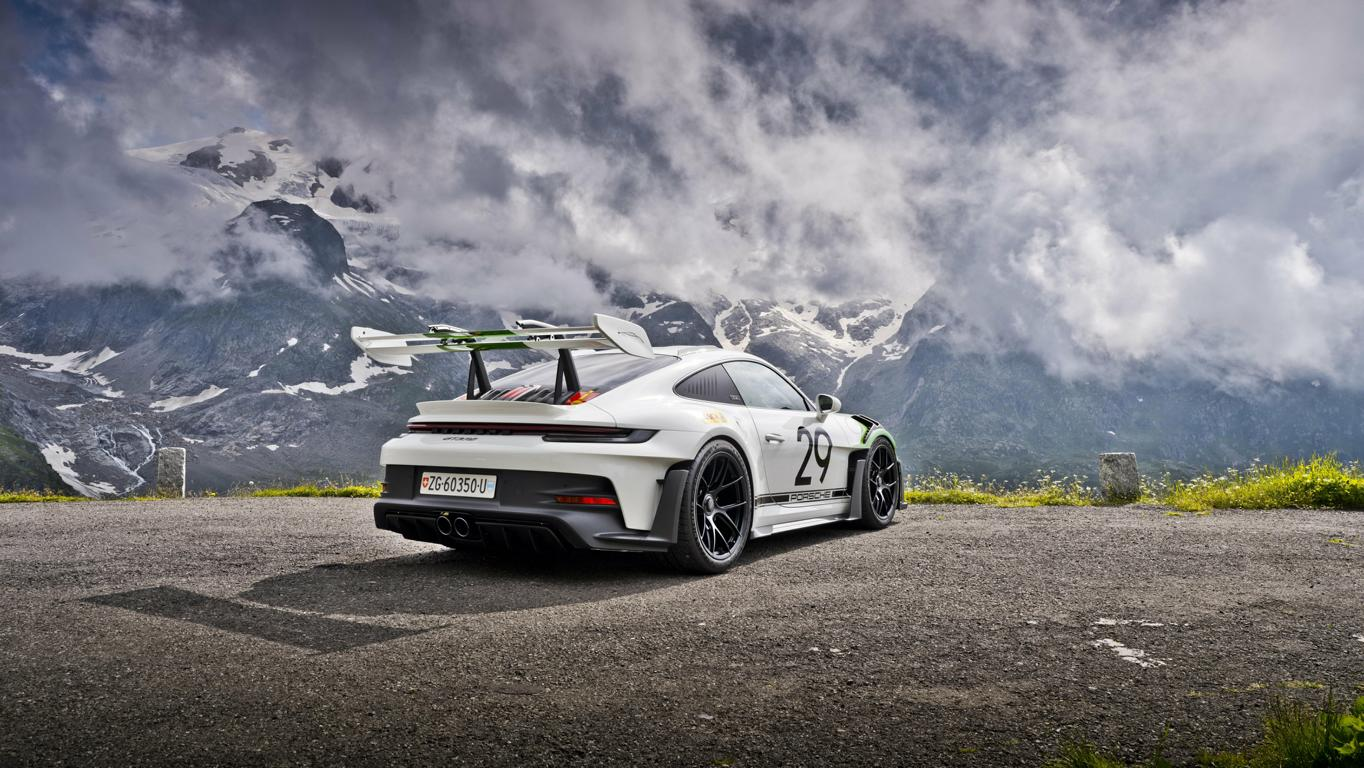
\includegraphics[width=\textwidth]{Porsche.jpg}
    \caption{Unten links}
  \end{subfigure}
  \hfill
  \begin{subfigure}[b]{0.45\textwidth}
    \centering
    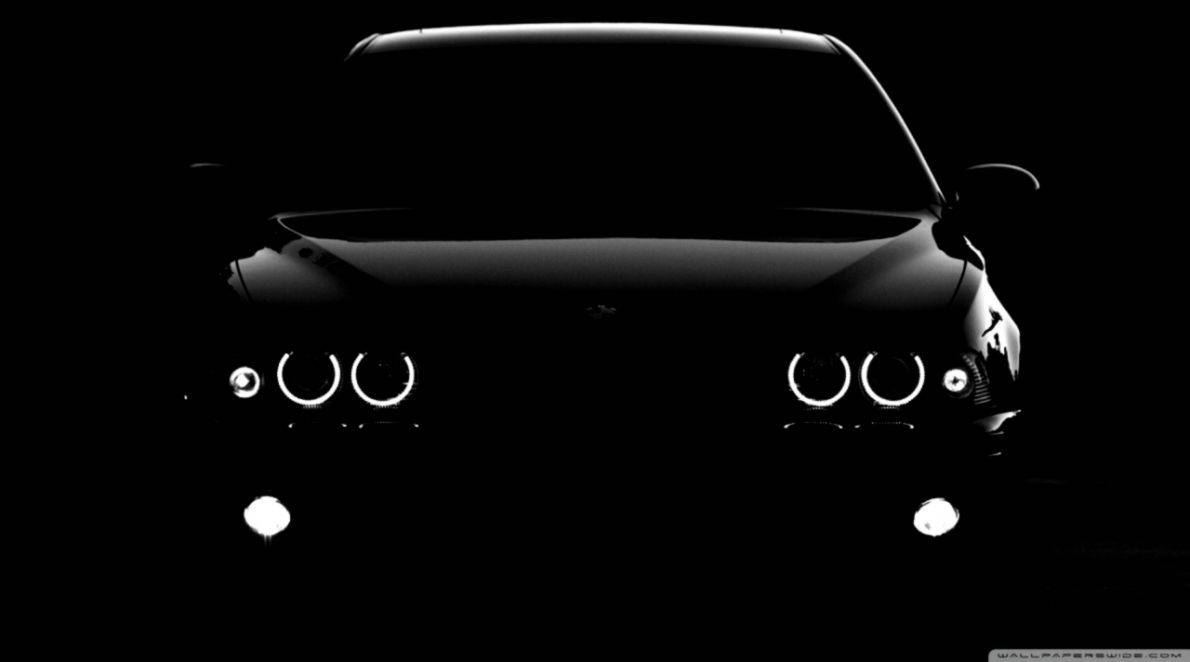
\includegraphics[width=\textwidth]{BMW.jpg}
    \caption{Unten rechts}
  \end{subfigure}
  \caption{2×2 Grid mit vier Unterabbildungen.}
  \label{fig:grid-2x2}
\end{figure}

\subsubsection{Unterschiedliche Größen bei Unterabbildungen}
\begin{figure}[H]
  \centering
  % Asymmetrisches Layout: ein großes und ein kleines Bild
  % Wichtig: Summe der Breiten + Abstände ≤ 100%
  \begin{subfigure}[b]{0.6\textwidth}
    \centering
    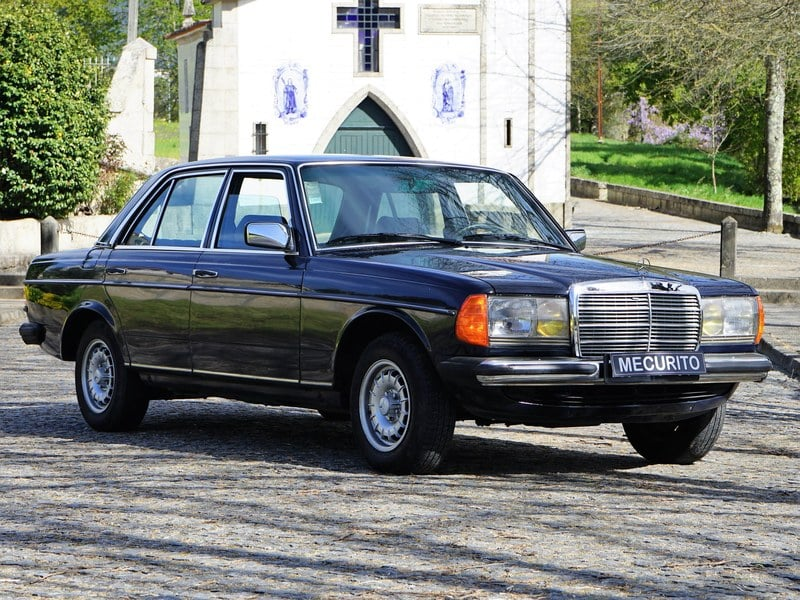
\includegraphics[width=\textwidth]{Mercedes.jpg}
    \caption{Großes Hauptbild (60\%)}
  \end{subfigure}
  \hfill
  % \hfill passt den Abstand automatisch an
  \begin{subfigure}[b]{0.35\textwidth}
    \centering
    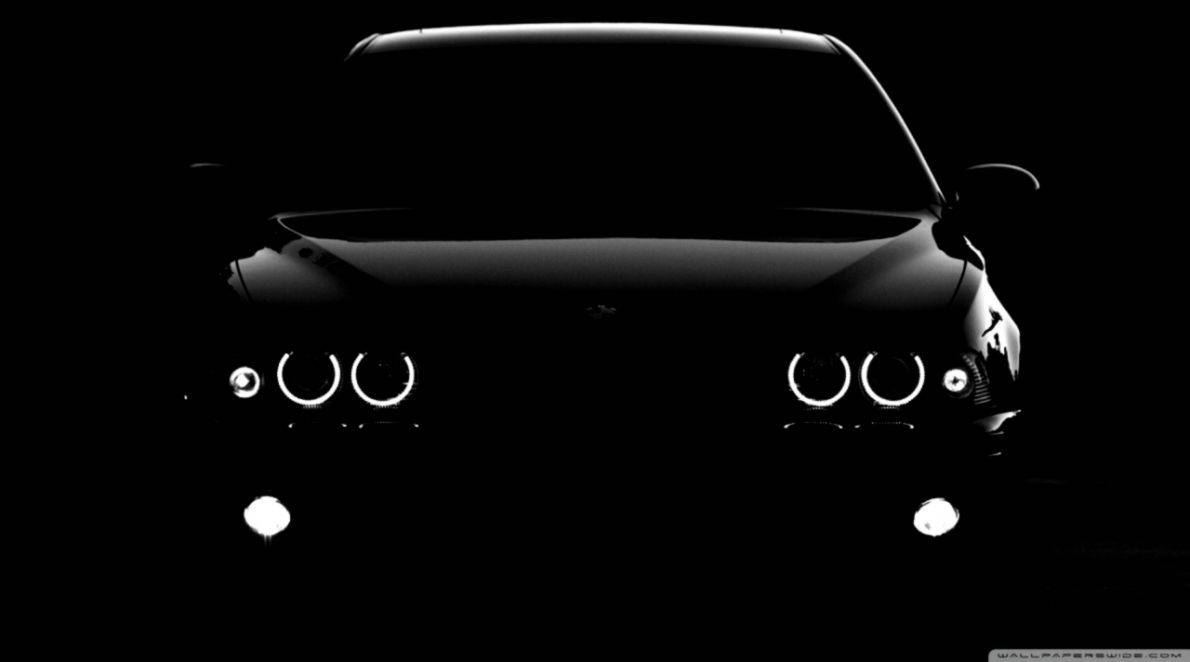
\includegraphics[width=\textwidth]{BMW.jpg}
    \caption{Kleineres Nebenbild (35\%)}
  \end{subfigure}
  \caption{Unterabbildungen mit unterschiedlichen Größen.}
\end{figure}

\vspace{1cm}
% =====================================================================
\subsection{Ausrichtung und Positionierung}
% Standardmäßig sind Abbildungen zentriert
% Mit speziellen Befehlen kann man die Ausrichtung ändern
% =====================================================================

\subsubsection{Linksbündige Abbildung}
\begin{figure}[H]
  \raggedright
  % \raggedright = linksbündig ausrichten, Text rechts unregelmäßig
  % Alternative zu \centering
  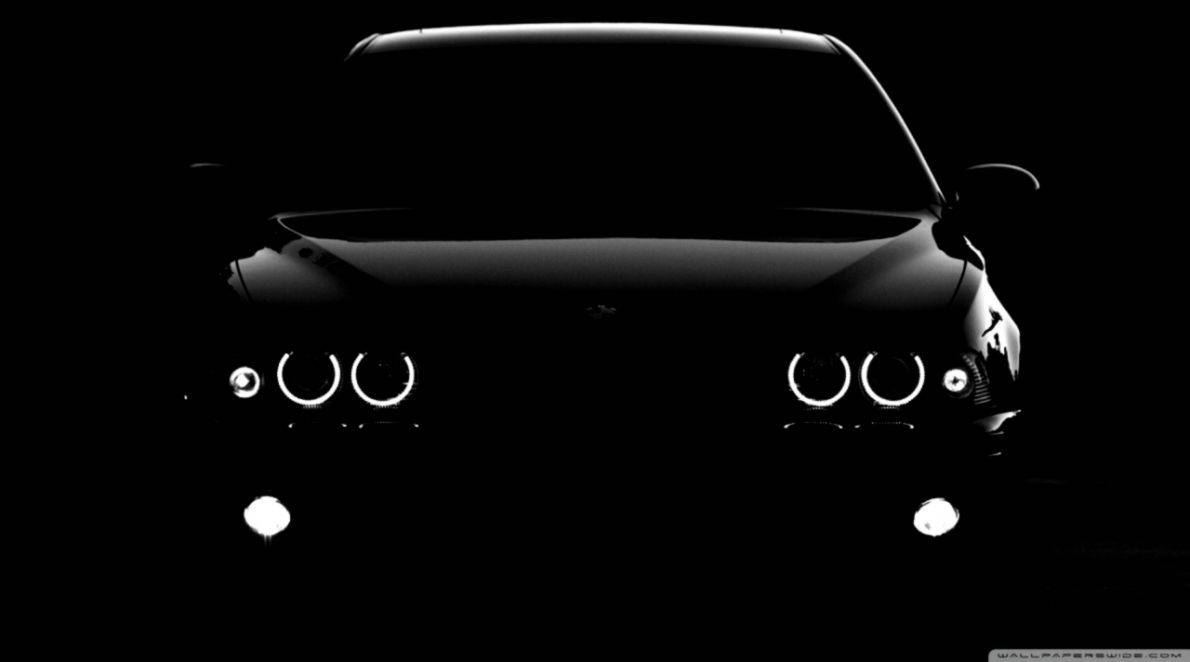
\includegraphics[width=0.5\textwidth]{BMW.jpg}
  \caption{Linksbündig ausgerichtete Abbildung.}
\end{figure}

\subsubsection{Rechtsbündige Abbildung}
\begin{figure}[H]
  \raggedleft
  % \raggedleft = rechtsbündig ausrichten, Text links unregelmäßig
  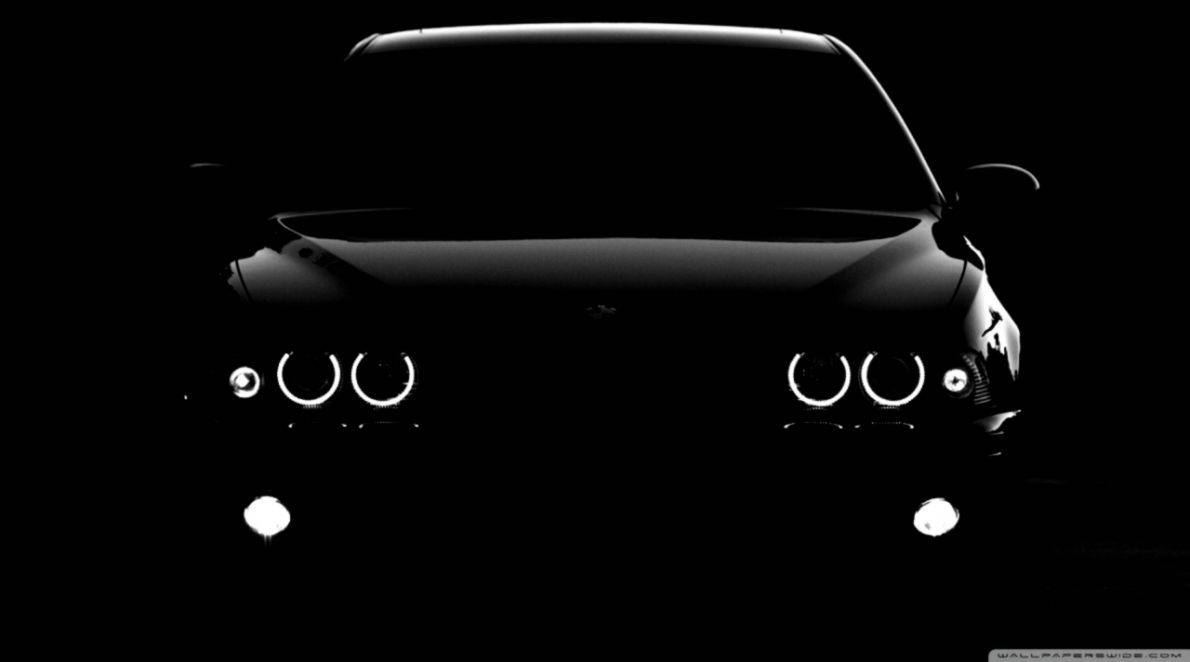
\includegraphics[width=0.5\textwidth]{BMW.jpg}
  \caption{Rechtsbündig ausgerichtete Abbildung.}
\end{figure}

\subsubsection{Zentrierte Abbildung (Standard)}
\begin{figure}[H]
  \centering
  % \centering = horizontal zentriert (Standard in den meisten Fällen)
  % Bildunterschrift wird ebenfalls zentriert
  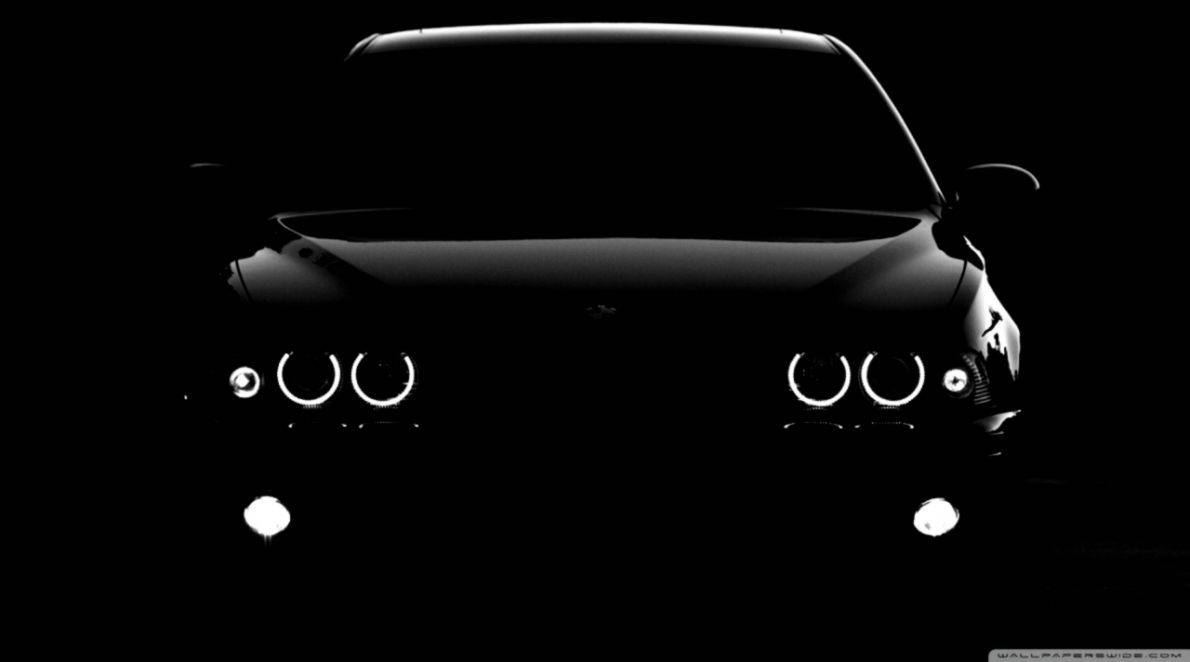
\includegraphics[width=0.5\textwidth]{BMW.jpg}
  \caption{Zentriert (Standard-Ausrichtung).}
\end{figure}

\newpage
% =====================================================================
\subsection{Textumlauf mit wrapfig}
% Das wrapfig-Paket ermöglicht Textumlauf um Abbildungen
% Ideal für kleinere Bilder in längeren Textpassagen
% =====================================================================

\subsubsection{Rechtsbündiges Bild mit Textumlauf}
\begin{wrapfigure}{r}{0.5\textwidth}
  % {r} = rechtsbündig platzieren
  % Alternativen: {l} = links, {i} = innen (bei zweiseitigem Druck), {o} = außen
  % 0.4\textwidth = Gesamtbreite inkl. Abstand zum Text
  \centering
  \vspace{-10pt}
  % Negativer vertikaler Abstand = Bild näher zum Text bewegen
  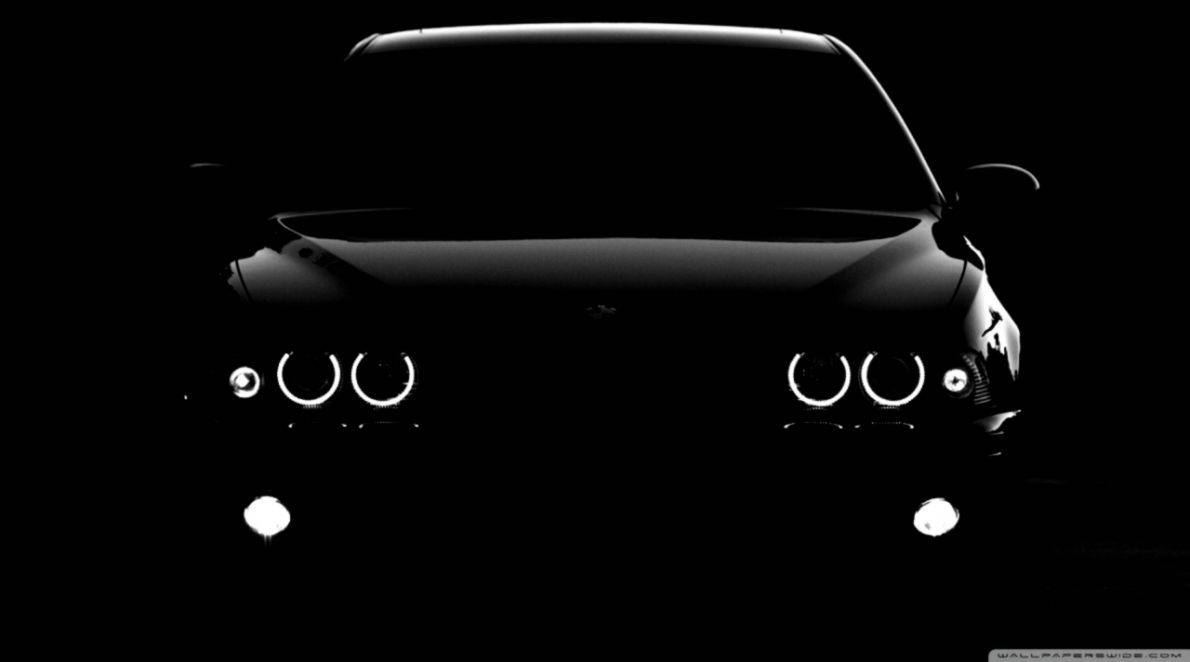
\includegraphics[width=0.32\textwidth]{BMW.jpg}
  % Bildbreite etwas kleiner als wrapfigure-Breite (Abstand zum Text)
  \caption{BMW rechts}
  \vspace{-10pt}
  % Abstand nach dem Bild reduzieren
\end{wrapfigure}

% Text fließt automatisch um das Bild herum
Die Bayerische Motoren Werke AG (BMW) ist ein deutscher Automobil- und Motorradhersteller mit Sitz in München. Das Unternehmen wurde 1916 gegründet und steht heute weltweit für Premiumfahrzeuge, Innovation und Fahrdynamik. Besonders bekannt ist BMW für den charakteristischen Doppelnieren-Kühlergrill und das sportliche Fahrverhalten seiner Modelle. Die Marke verbindet technische Präzision mit elegantem Design. Durch die wrapfig-Umgebung fließt der Text automatisch um das Bild herum.

\vspace{1cm} % Abstand zwischen den beiden Beispielen  
\subsubsection{Linksbündiges Bild mit Textumlauf}
\begin{wrapfigure}{l}{0.5\textwidth}
  % {l} = linksbündig, Text fließt rechts am Bild vorbei
  \centering
  \vspace{-10pt}
  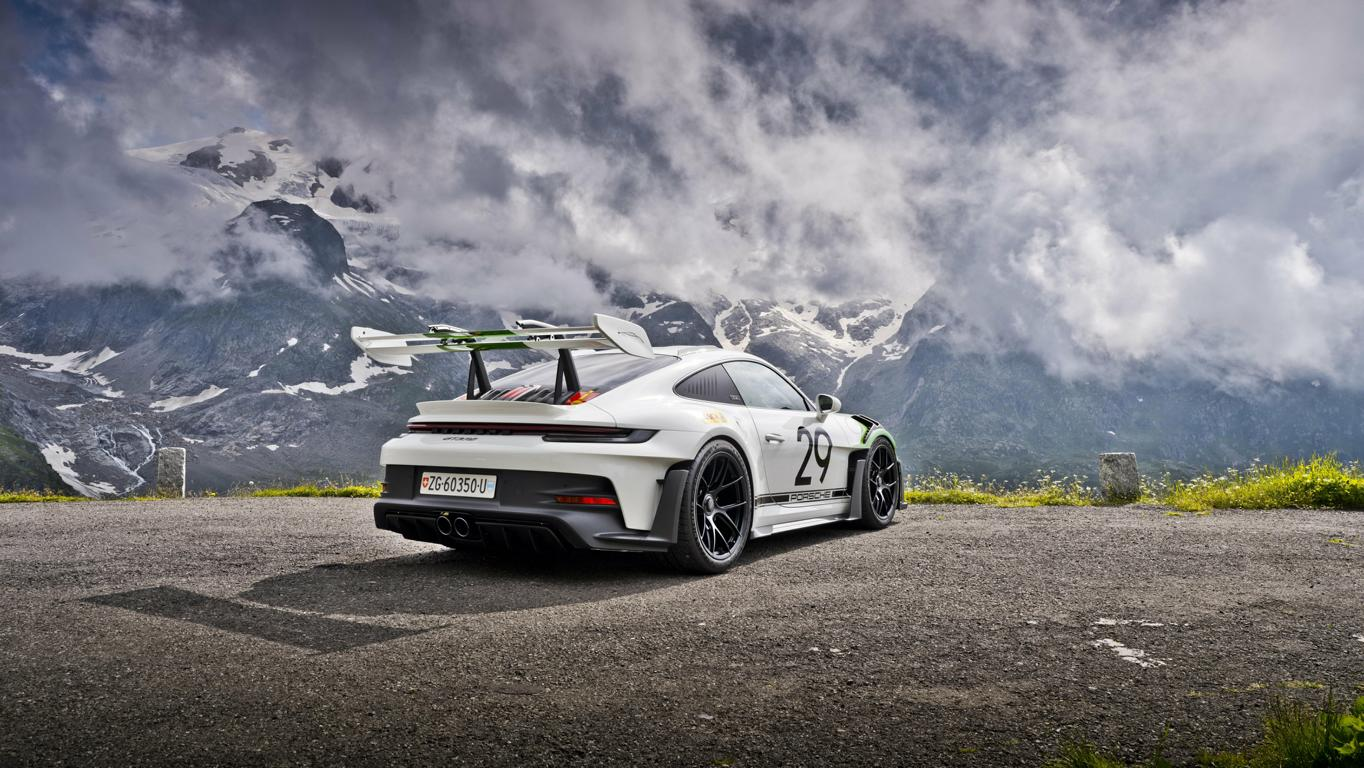
\includegraphics[width=0.32\textwidth]{Porsche.jpg}
  \caption{Porsche links}
  \vspace{-10pt}
\end{wrapfigure}

% WICHTIG: Nach \begin{wrapfigure} muss genug Text folgen!
% Mindestens so viel, wie die Bildhöhe + Bildunterschrift einnimmt
Die Dr. Ing. h.c. F. Porsche AG ist ein deutscher Sportwagenhersteller mit Sitz in Stuttgart-Zuffenhausen. Das Unternehmen wurde 1931 von Ferdinand Porsche gegründet und ist heute bekannt für seine ikonischen Sportwagenmodelle wie den 911. Porsche steht für Ingenieurskunst auf höchstem Niveau und verbindet Leistung mit Alltagstauglichkeit. Der Text umfließt hier das linksbündig platzierte Bild auf natürliche Weise.

% =====================================================================
\subsection{Gedrehte und querformatige Abbildungen}
% Für breite Grafiken, die besser im Querformat dargestellt werden
% Benötigt das rotating-Paket
% =====================================================================

\subsubsection{Um 90° gedrehte Abbildung (Querformat)}
\begin{sidewaysfigure}
  % sidewaysfigure dreht die gesamte Figure-Umgebung um 90°
  % Die Seite bleibt im Hochformat, nur die Abbildung wird gedreht
  % Ideal für breite Diagramme, Tabellen oder Panoramabilder
  \centering
  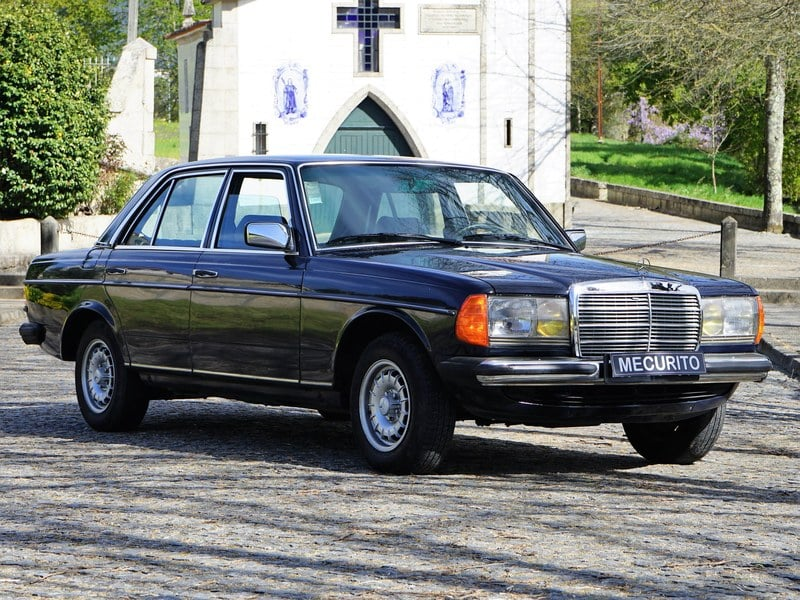
\includegraphics[width=0.7\textheight]{Mercedes.jpg}
  % ACHTUNG: width bezieht sich auf \textheight (Höhe wird zur Breite)
  % Bei Drehung: Texthöhe = neue Breite, Textbreite = neue Höhe
  \caption{Diese Abbildung ist um 90° gedreht (ideal für breite Grafiken).}
  \label{fig:gedreht}
\end{sidewaysfigure}

\newpage

% =====================================================================
\subsection{Bildunterschriften und Beschriftungen}
% Verschiedene Arten von Captions für unterschiedliche Anforderungen
% =====================================================================

\subsubsection{Kurze und lange Bildunterschriften}
\begin{figure}[H]
  \centering
  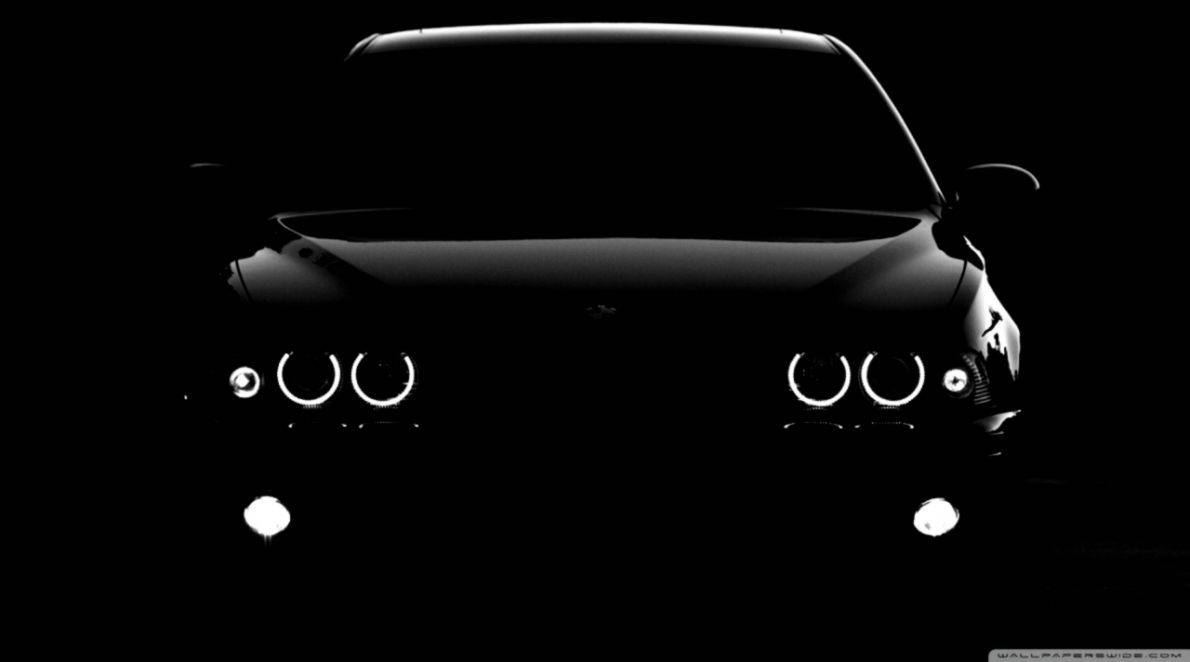
\includegraphics[width=0.5\textwidth]{BMW.jpg}
  \caption[Kurztitel für Abbildungsverzeichnis]{Dies ist eine sehr lange Bildunterschrift, die im Abbildungsverzeichnis nur als Kurztitel erscheint, im Dokument selbst aber vollständig angezeigt wird. So bleibt das Verzeichnis übersichtlich.}
  % Syntax: \caption[Kurzversion]{Langversion}
  % Kurzversion erscheint im \listoffigures
  % Langversion erscheint unter der Abbildung im Dokument
\end{figure}

\subsubsection{Bildunterschrift mit Quellenangabe}
\begin{figure}[H]
  \centering
  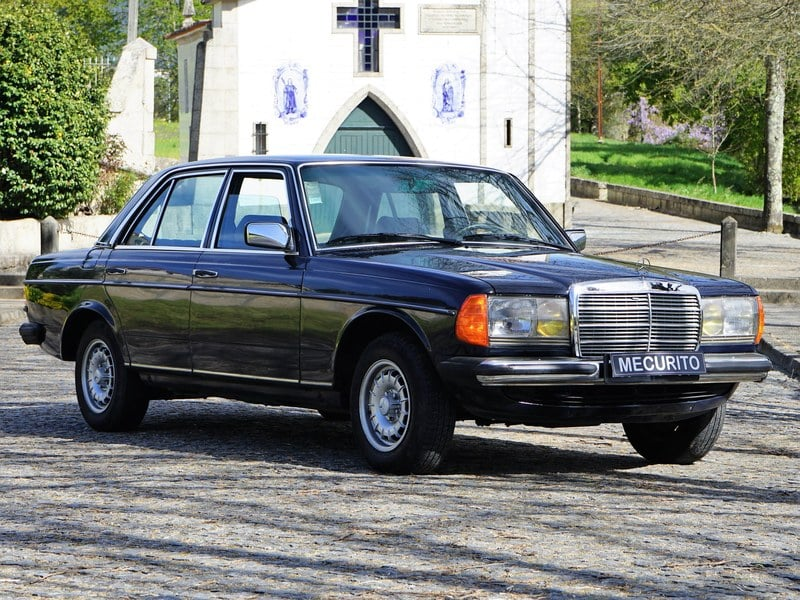
\includegraphics[width=0.5\textwidth]{Mercedes.jpg}
  \caption{Mercedes-Benz Fahrzeug. \textit{Quelle: Eigene Darstellung, 2025.}}
  % \textit{} für kursive Quellenangabe
  % Standard in wissenschaftlichen Arbeiten
  % Alternative: \caption{Text}\\\textit{Quelle: ...}
\end{figure}

\subsubsection{Bildunterschrift oberhalb des Bildes}
\begin{figure}[H]
  \centering
  \caption{Diese Bildunterschrift steht ÜBER dem Bild.}
  % Caption VOR \includegraphics = Caption oben
  % Manchmal in technischen Dokumenten gewünscht
  \vspace{0.3cm}
  % Abstand zwischen Caption und Bild
  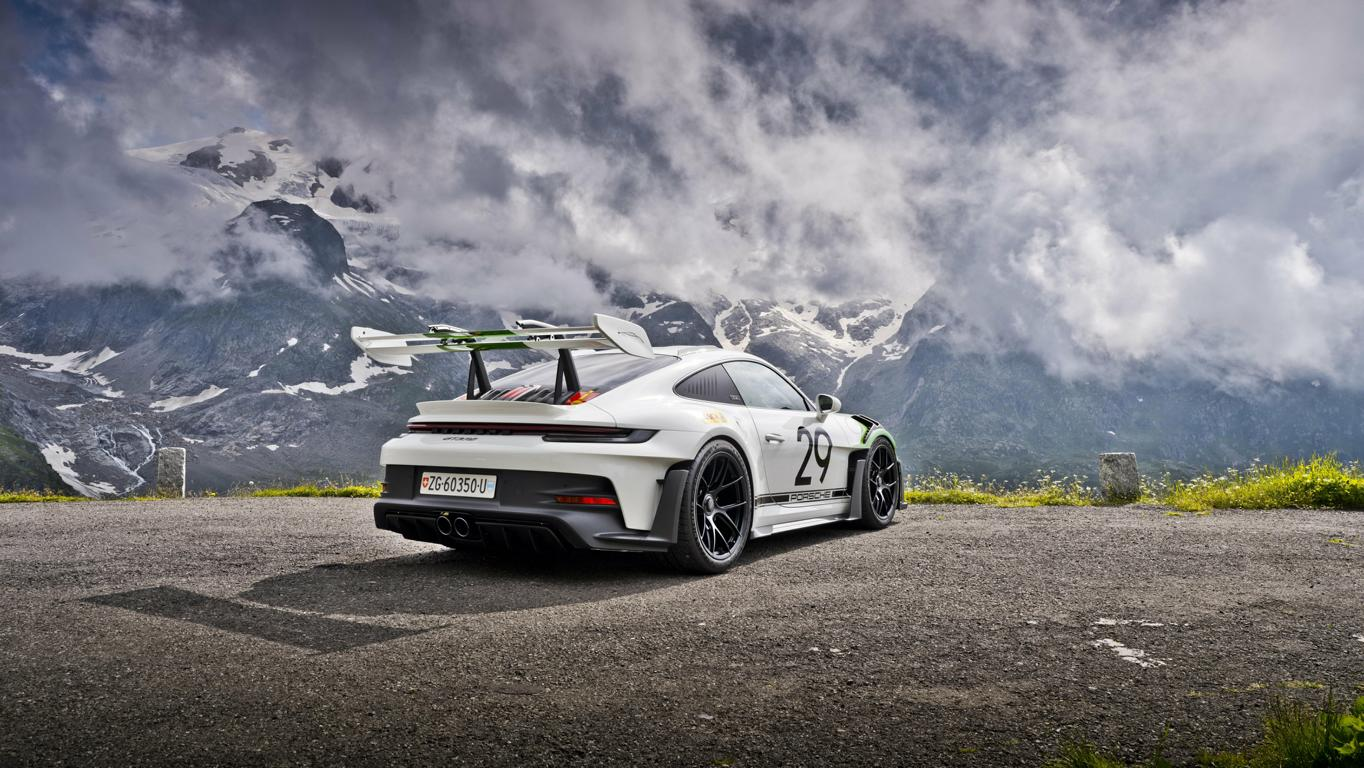
\includegraphics[width=0.5\textwidth]{Porsche.jpg}
\end{figure}

% =====================================================================
\subsection{Rahmen und Hintergründe}
% Visuelle Hervorhebung von Abbildungen
% Benötigt das xcolor-Paket für Farben
% =====================================================================

\subsubsection{Abbildung mit Rahmen}
\begin{figure}[H]
  \centering
  \fbox{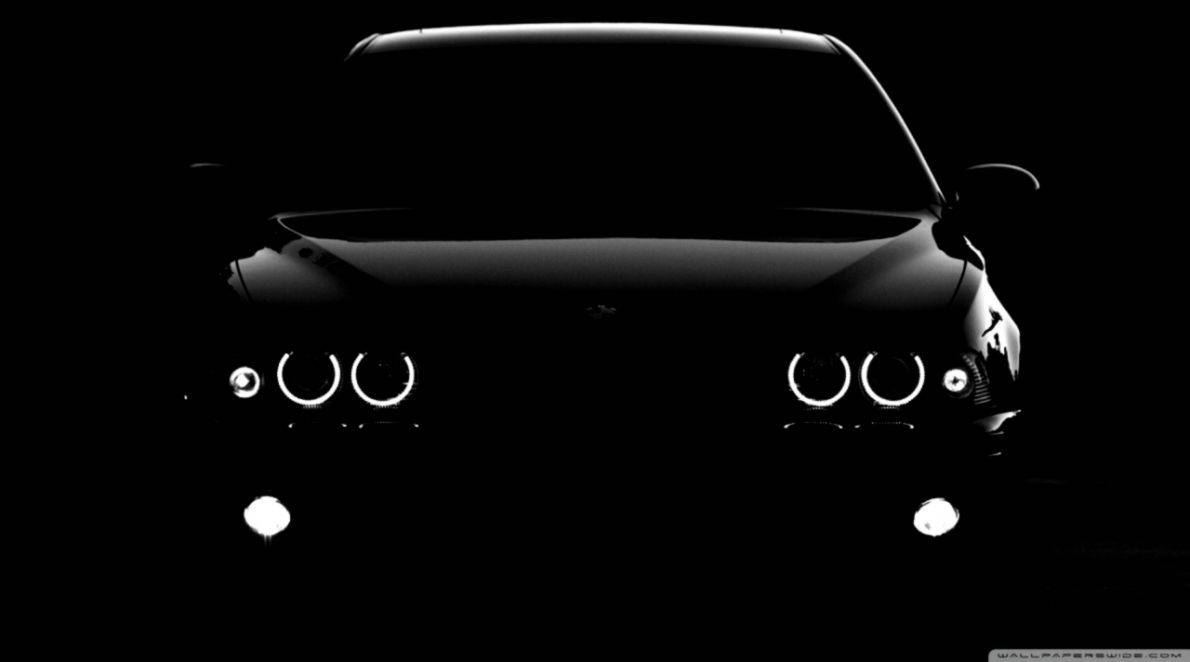
\includegraphics[width=0.5\textwidth]{BMW.jpg}}
  % \fbox{} = frame box = schwarzer Rahmen um den Inhalt
  % Standard-Rahmenstärke und -farbe
  % Rahmen passt sich automatisch an die Bildgröße an
  \caption{Abbildung mit schwarzem Rahmen (fbox).}
\end{figure}

\subsubsection{Abbildung mit farbigem Rahmen}
\begin{figure}[H]
  \centering
  \fcolorbox{blue}{white}{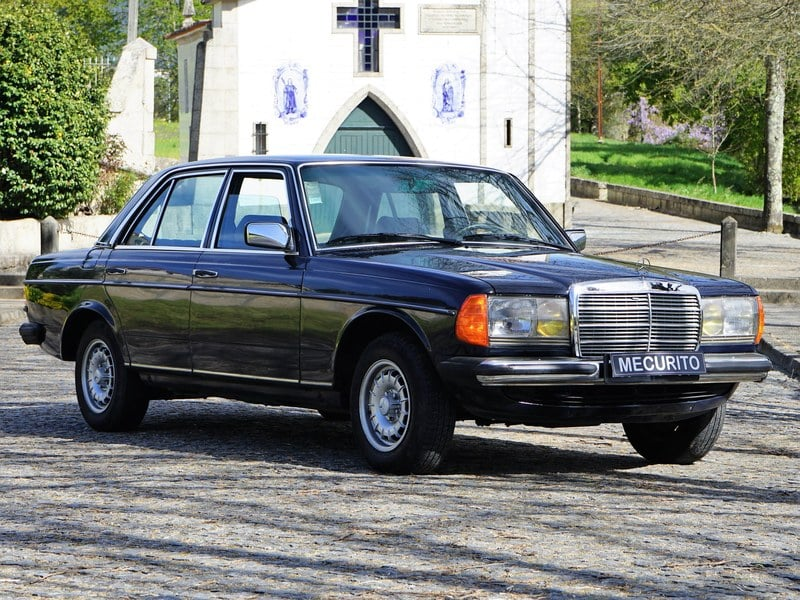
\includegraphics[width=0.5\textwidth]{Mercedes.jpg}}
  % \fcolorbox{Rahmenfarbe}{Hintergrundfarbe}{Inhalt}
  % {blue} = blaue Rahmenfarbe
  % {white} = weißer Hintergrund (transparent zum Dokument)
  % Weitere Farben: red, green, yellow, cyan, magenta, black, etc.
  \caption{Abbildung mit blauem Rahmen.}
\end{figure}

\subsubsection{Abbildung mit Hintergrundfarbe}
\begin{figure}[H]
  \centering
  \colorbox{yellow!30}{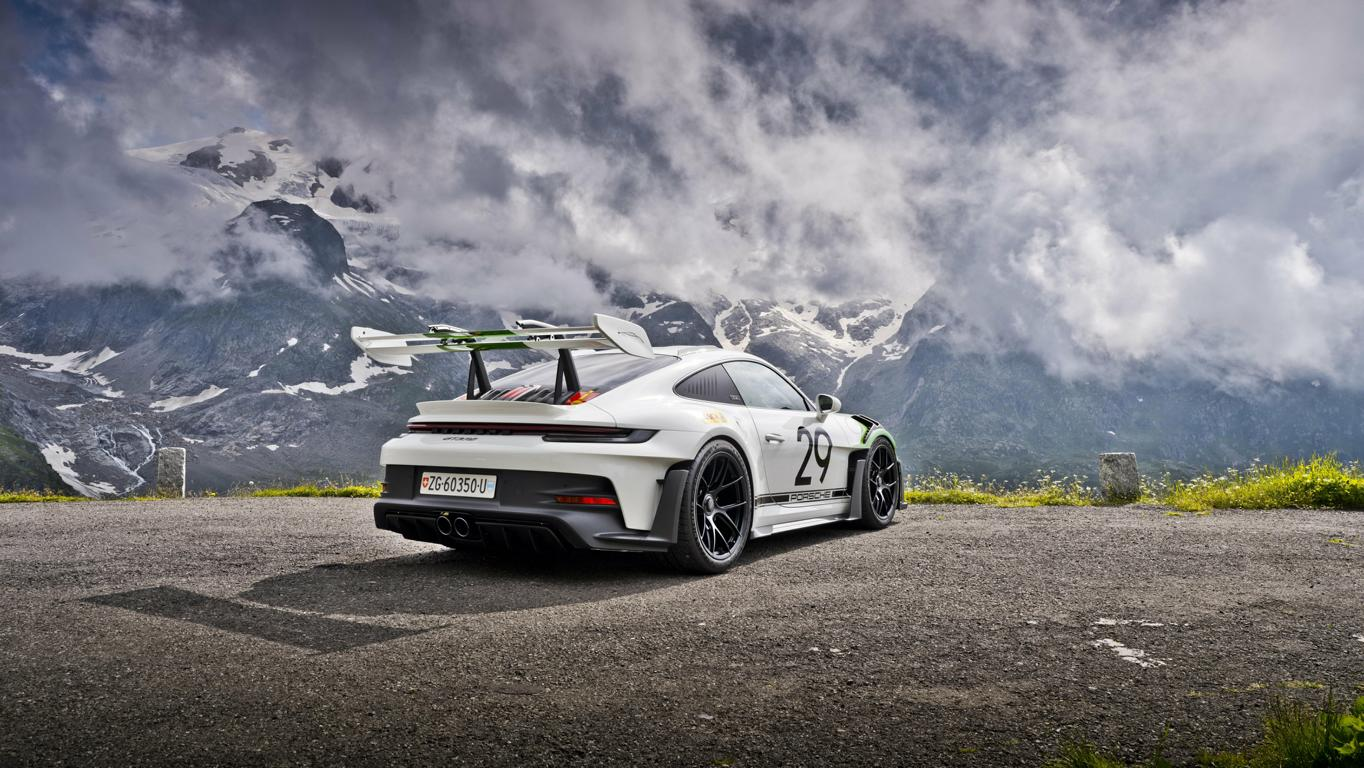
\includegraphics[width=0.5\textwidth]{Porsche.jpg}}
  % \colorbox{Farbe}{Inhalt} = nur Hintergrundfarbe, kein Rahmen
  % yellow!30 = 30% Gelb (gemischt mit Weiß) = helles Gelb
  % Syntax: Farbe!Prozent für Transparenz/Helligkeit
  \caption{Abbildung mit gelbem Hintergrund.}
\end{figure}

\subsubsection{Mehrere Abbildungen untereinander}
\begin{figure}[H]
  \centering
  % Drei Bilder vertikal gestapelt in einer Figure
  % Vorteil: gemeinsame Nummerierung, eine Caption
  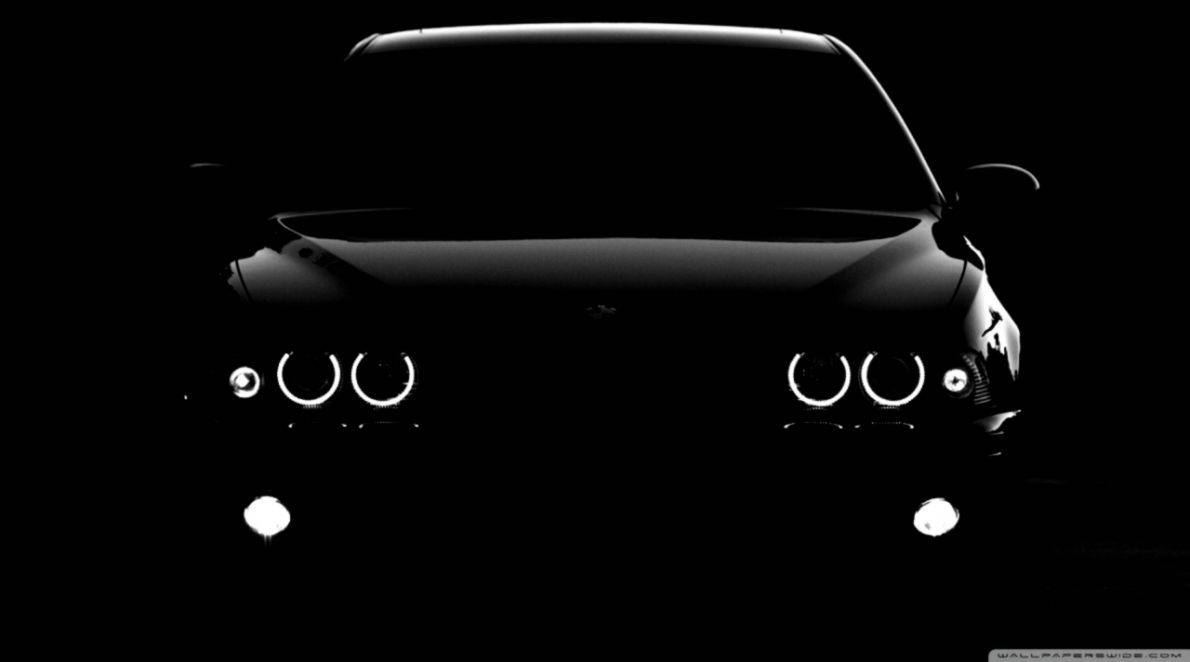
\includegraphics[width=0.45\textwidth]{BMW.jpg}
  \vspace{0.5cm}
  % Vertikaler Abstand zwischen den Bildern
  
  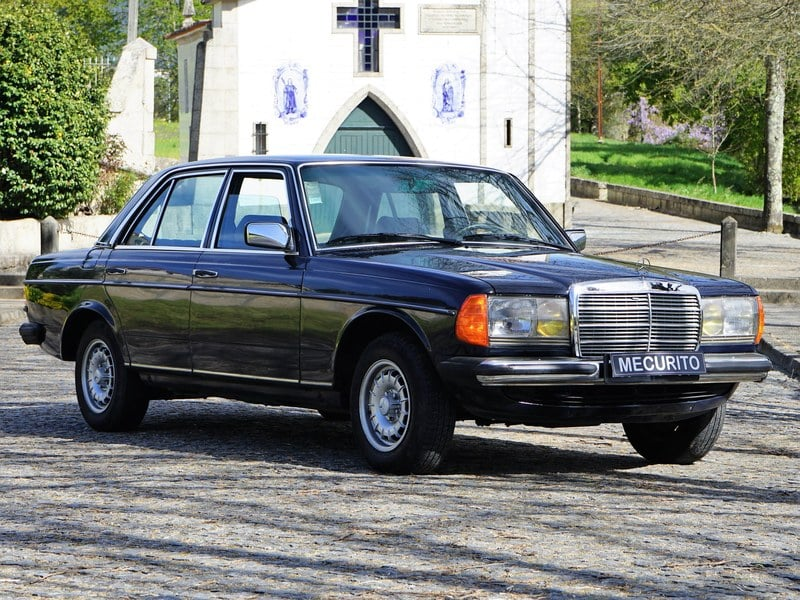
\includegraphics[width=0.45\textwidth]{Mercedes.jpg}
  \vspace{0.5cm}
  
  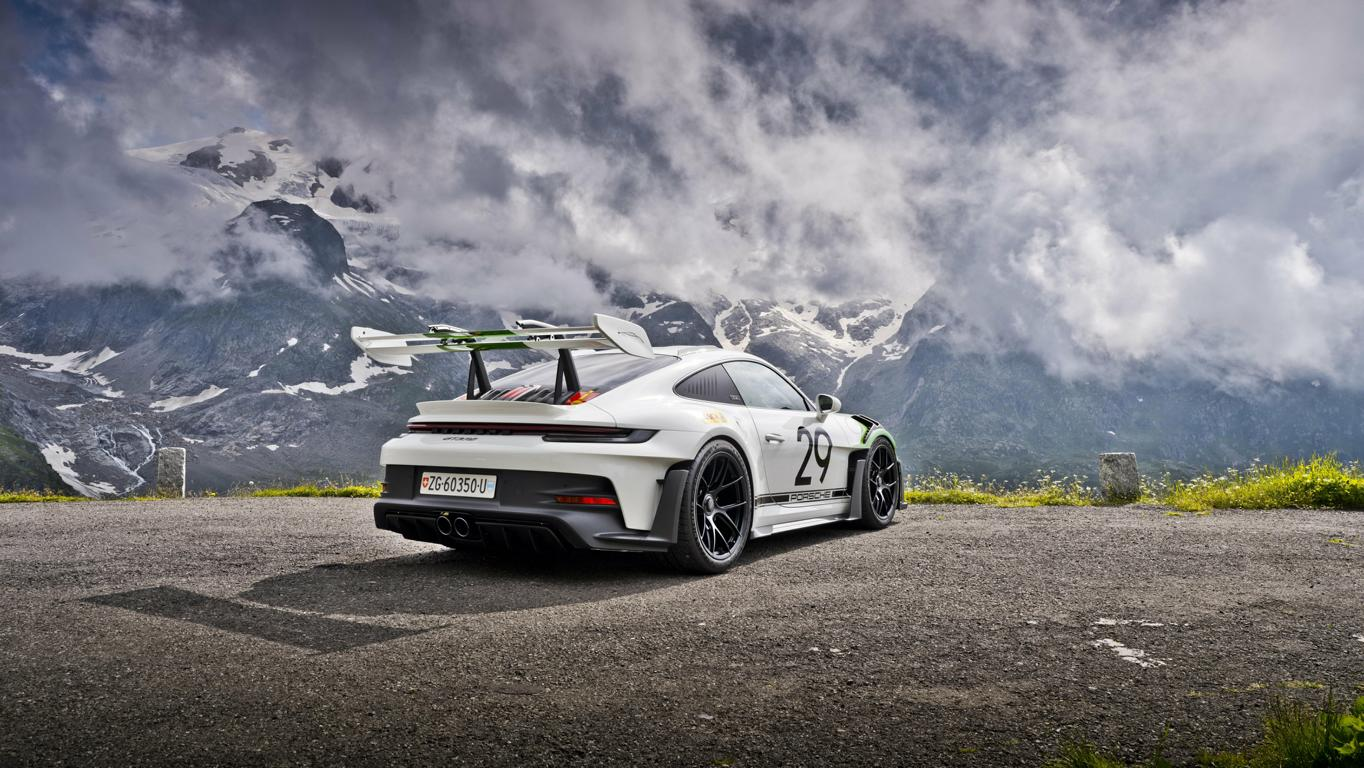
\includegraphics[width=0.45\textwidth]{Porsche.jpg}
  \caption{Drei Abbildungen vertikal gestapelt in einer Figure-Umgebung.}
  % Eine gemeinsame Bildunterschrift für alle drei Bilder
\end{figure}

% =====================================================================
\subsection{PDF-Dateien einbinden}
% PDFs können als ganze Seiten oder als Bilder eingefügt werden
% Benötigt das pdfpages-Paket
% =====================================================================

\subsubsection{Einzelne PDF-Seite einfügen}
% \includepdf fügt PDF-Seiten im Vollformat ein (ganze Seite)
% Ideal für Anhänge, externe Dokumente, Diagramme
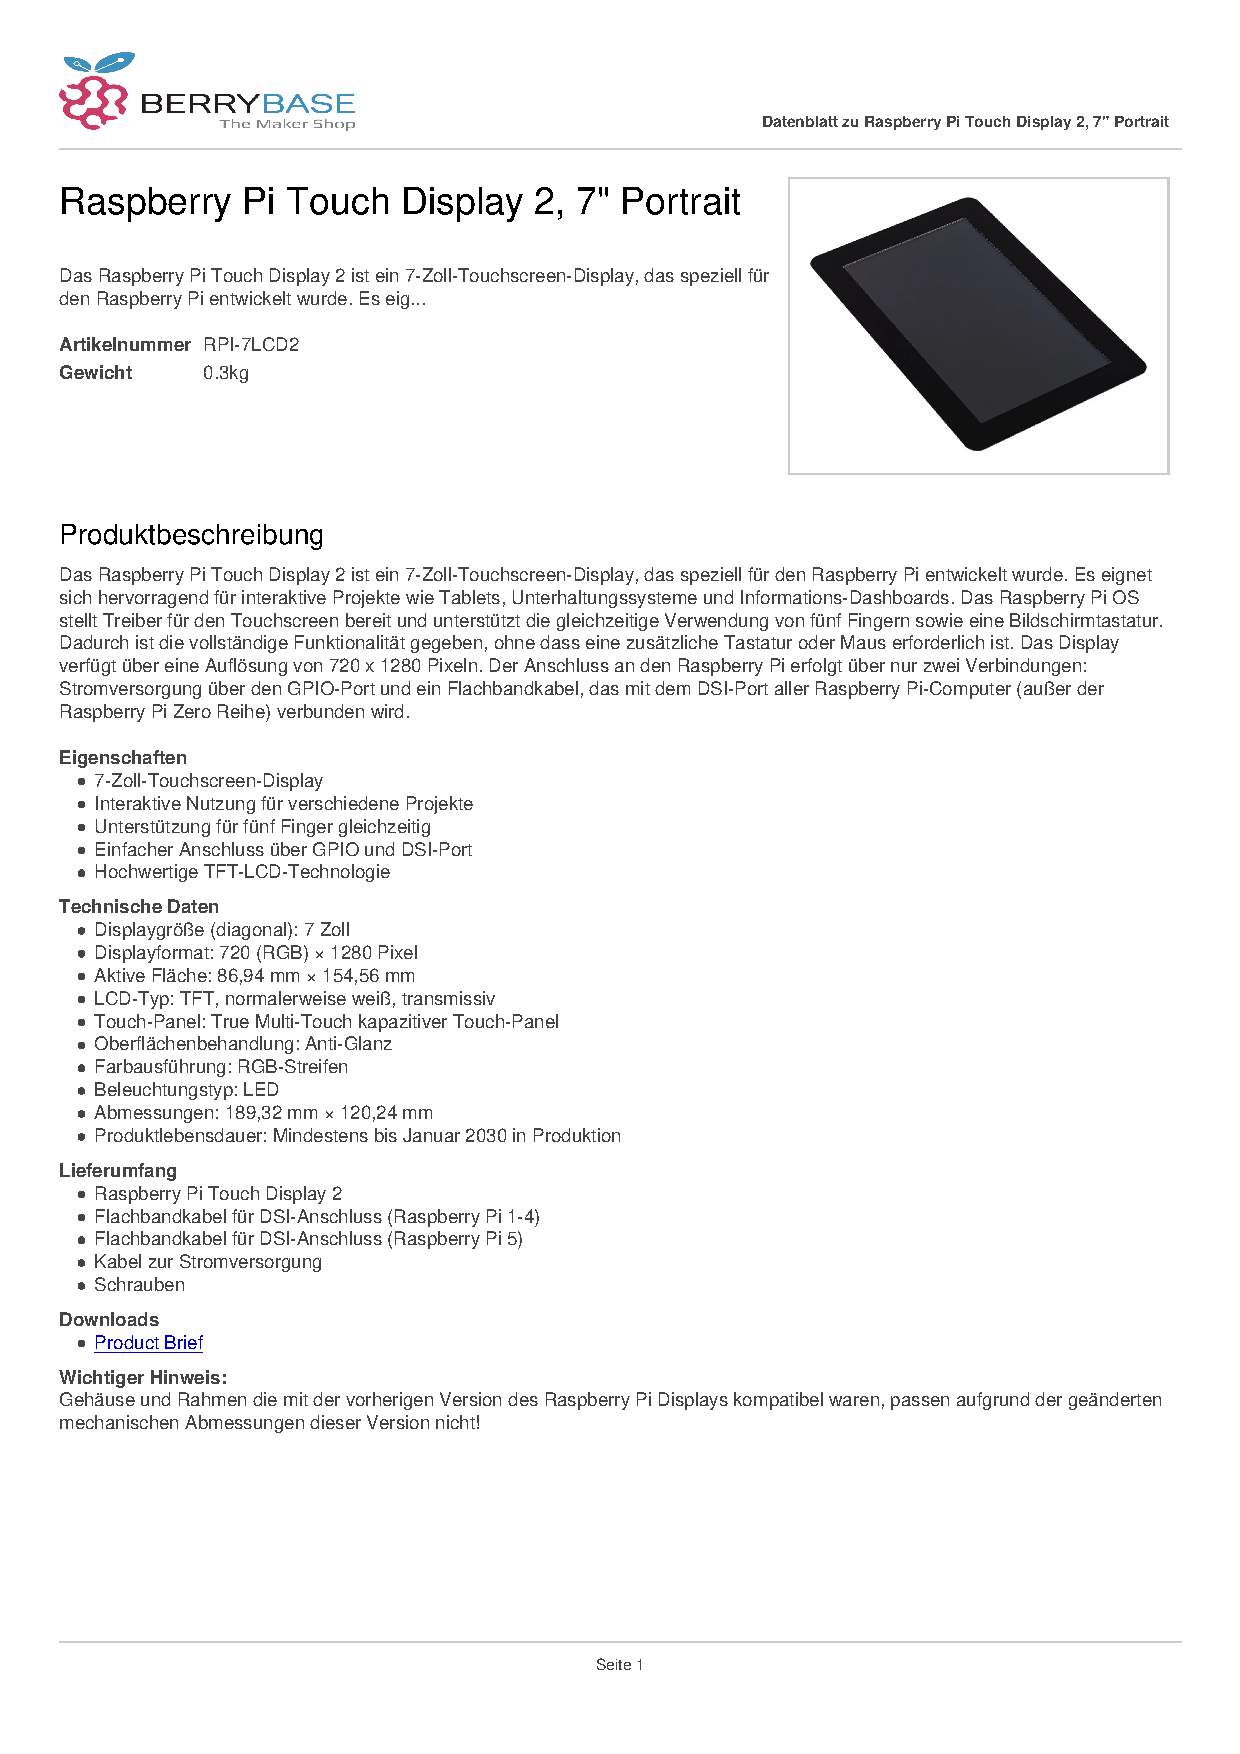
\includepdf[pages=1,scale=0.7,pagecommand={\subsection{Eingefügte PDF-Seite 1}}]{../ZPDF/Raspberry_Display.pdf}
% pages=1 = nur erste Seite einfügen
% scale=0.8 = auf 80% skalieren
% pagecommand={} = führt Befehle auf der eingefügten Seite aus

% Kommentar: Würde Seiten 1-3 einfügen 
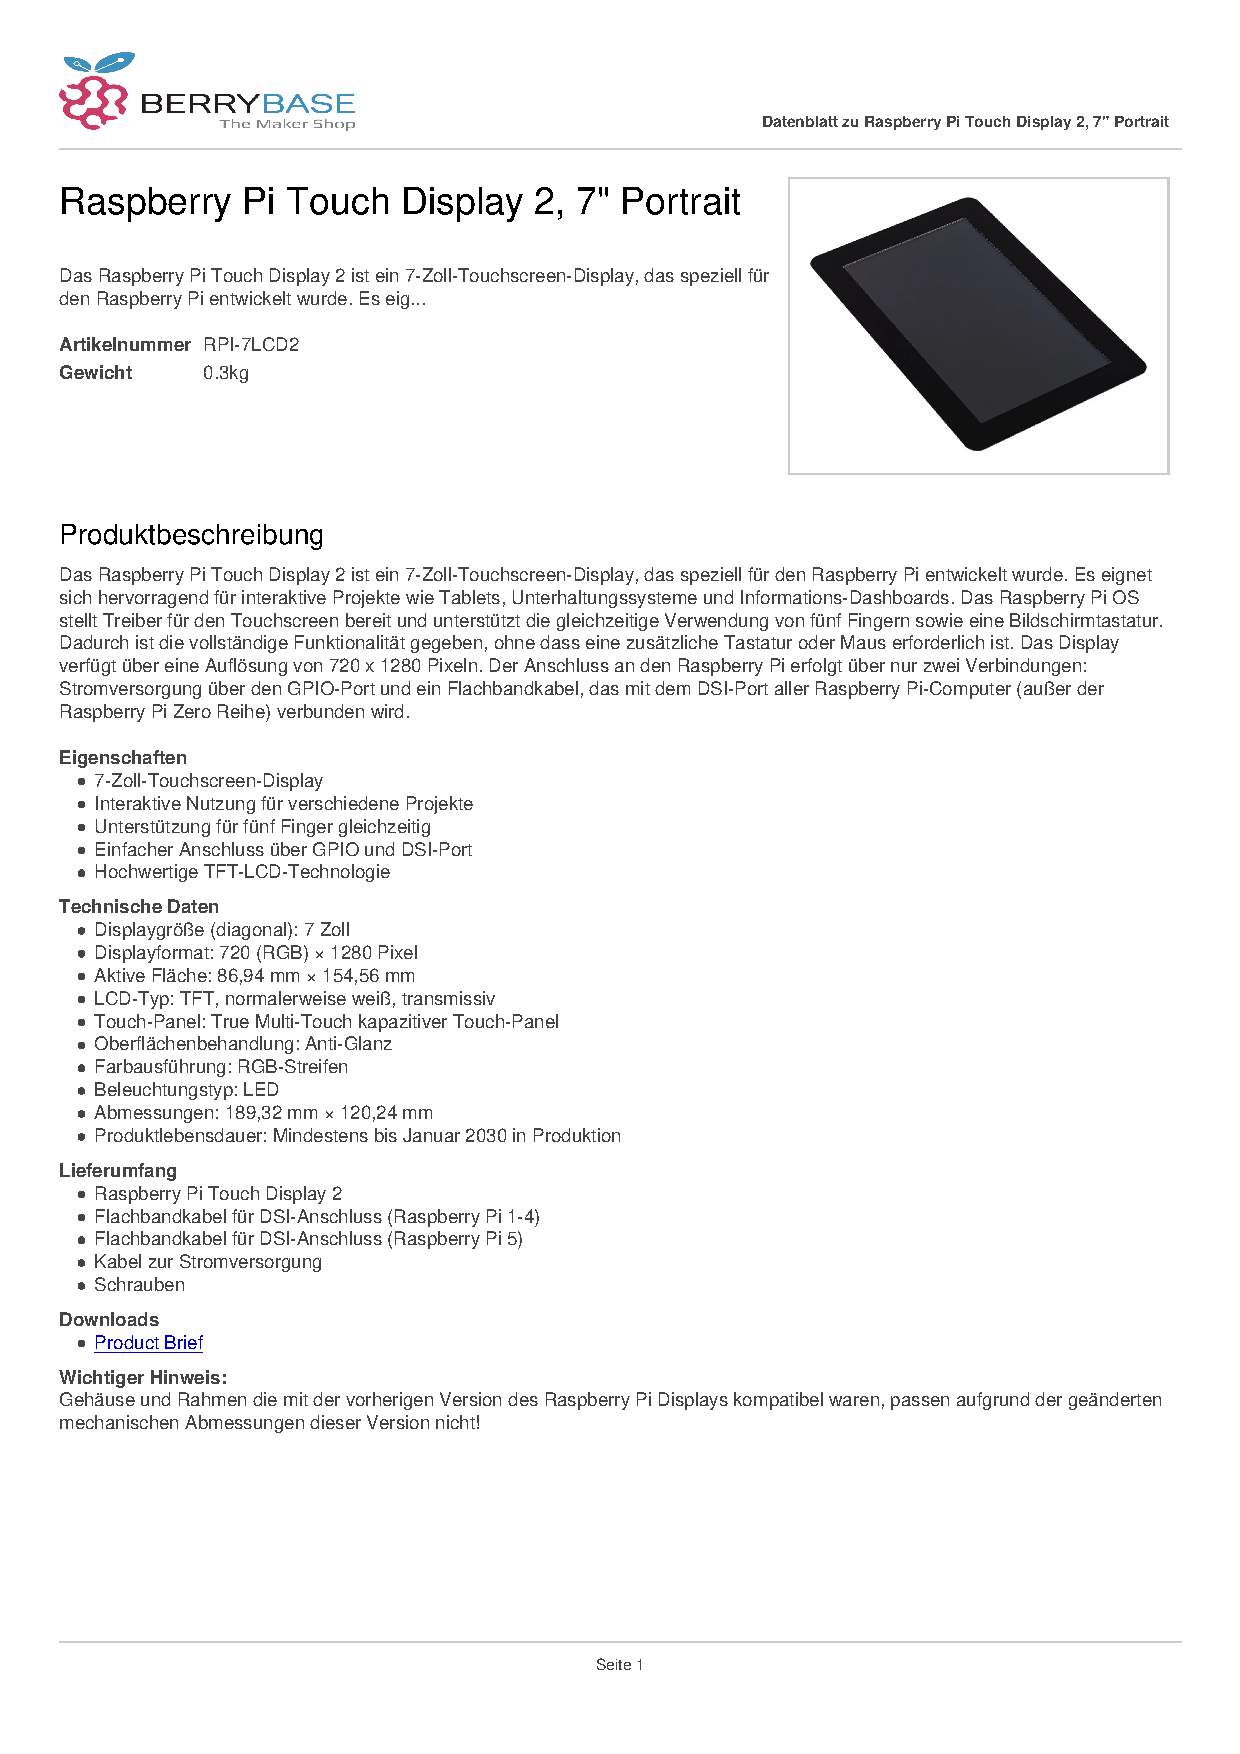
\includepdf[pages=1-3,scale=0.7,pagecommand=\subsection{Mehrere PDF-Seiten}]{../ZPDF/Raspberry_Display.pdf}
% pages=1-3 = Seiten 1 bis 3
% pages=- = alle Seiten
% pages={1,3,5} = nur Seiten 1, 3 und 5

% =====================================================================
\subsection{Fortgeschrittene Techniken}
% Spezielle Tricks und weniger bekannte Funktionen
% =====================================================================

\subsubsection{Abbildungen ohne Nummerierung}
\begin{figure}[H]
  \centering
  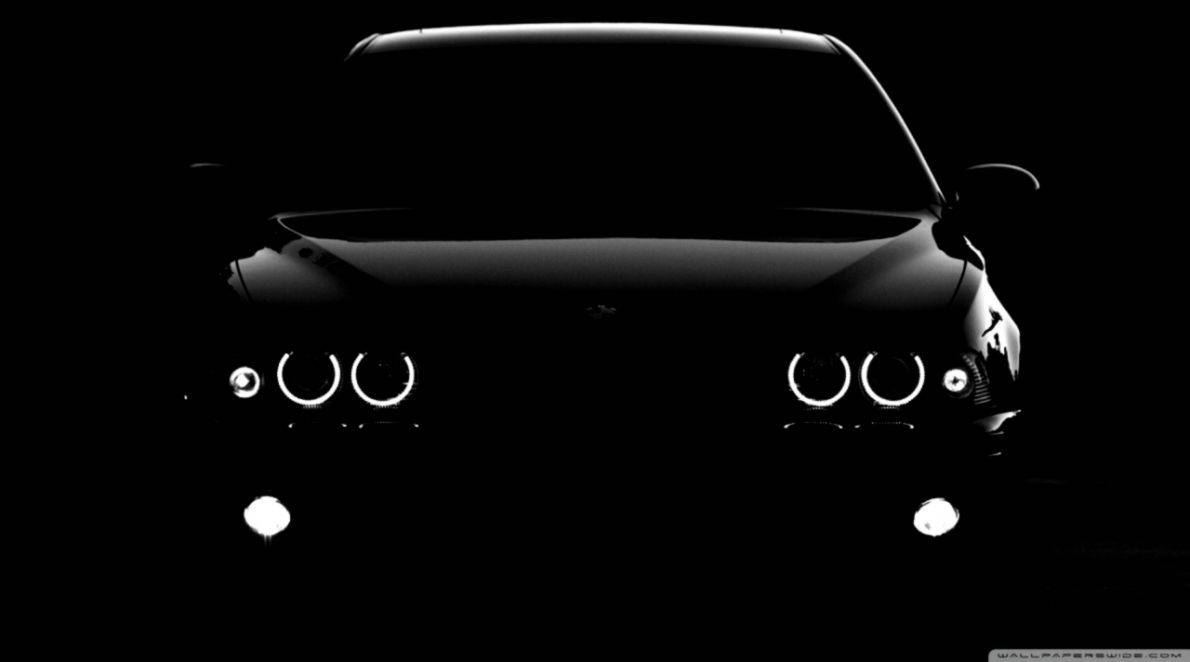
\includegraphics[width=0.5\textwidth]{BMW.jpg}
  \caption*{Unnummerierte Bildunterschrift (mit caption*).}
  % caption* (mit Stern) unterdrückt die Nummerierung
  % Abbildung erscheint NICHT im Abbildungsverzeichnis
  % Nützlich für dekorative Bilder ohne wissenschaftlichen Bezug
\end{figure}

\subsubsection{Eigenes Abbildungsverzeichnis-Format}
\begin{figure}[H]
  \centering
  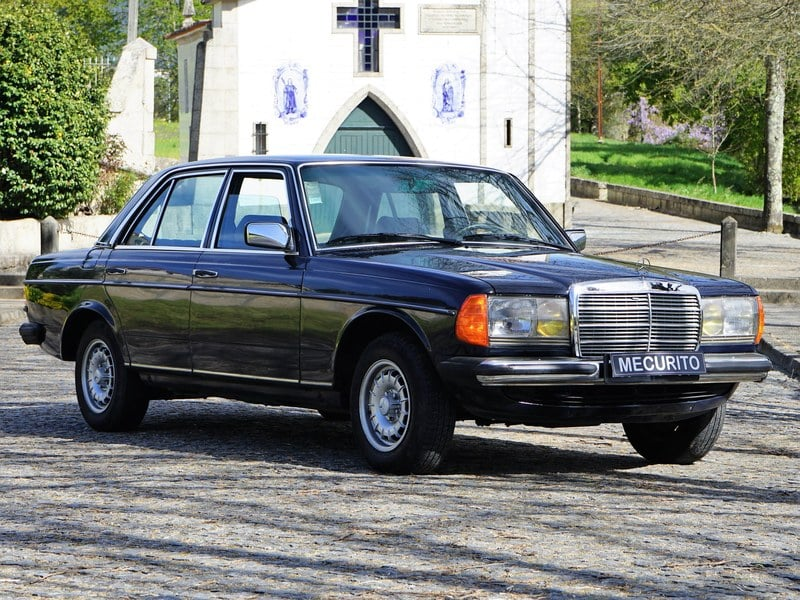
\includegraphics[width=0.5\textwidth]{Mercedes.jpg}
  \caption{Standard-Bildunterschrift mit Nummer.}
  % Normale Caption mit automatischer Nummerierung
  % Erscheint im \listoffigures
  \label{fig:standard-nummer}
\end{figure}

\subsubsection{Abbildung mit mehreren Labels}
\begin{figure}[H]
  \centering
  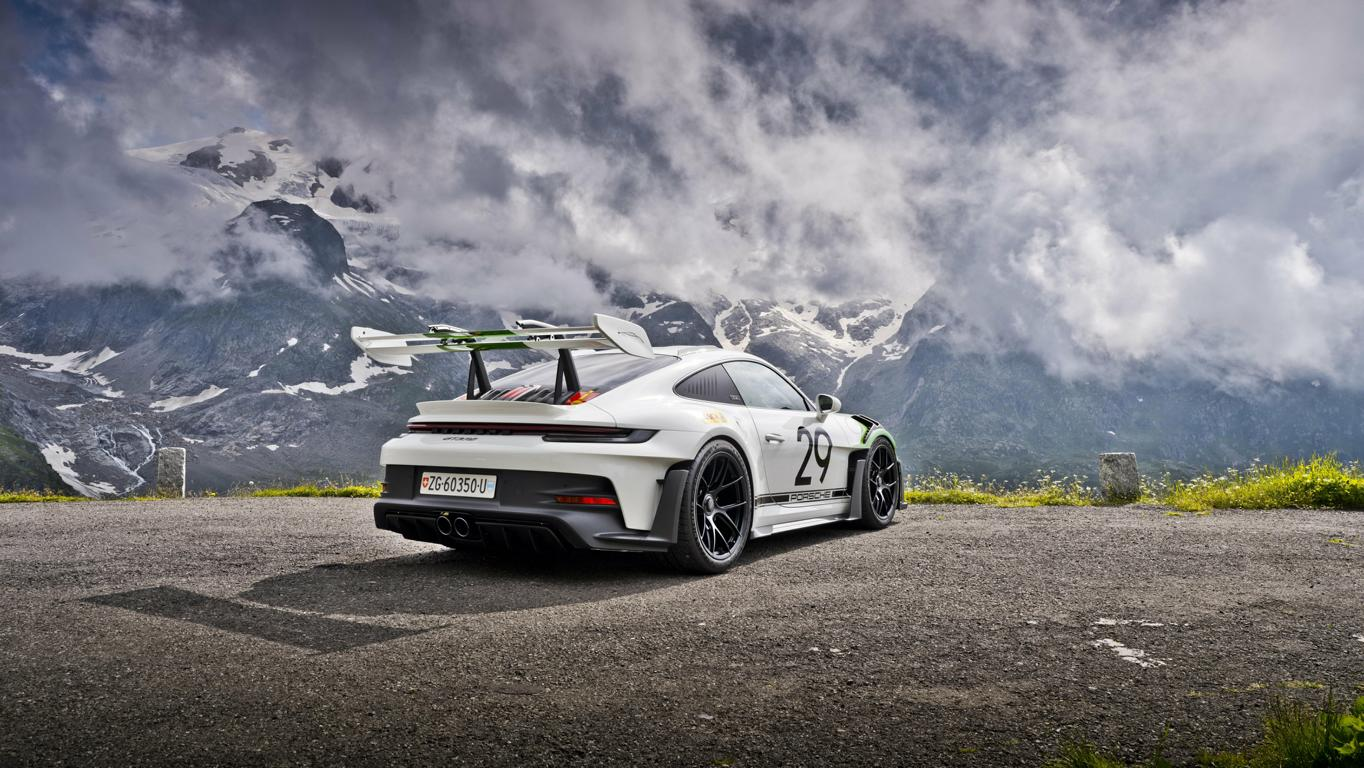
\includegraphics[width=0.5\textwidth]{Porsche.jpg}
  \caption{Abbildung mit Haupt-Label.}
  \label{fig:haupt}
  % Erstes Label
  \label{fig:alternativ}
  % Zweites Label für dieselbe Abbildung
  % Beide Labels verweisen auf die gleiche Nummer
\end{figure}
Referenz auf \ref{fig:haupt} oder \ref{fig:alternativ} zeigt die gleiche Abbildung.
% Nützlich wenn man verschiedene Perspektiven auf dasselbe Bild referenzieren will

\subsubsection{Floating vs. Non-Floating}
\begin{figure}[H]
  % [H] = Non-Floating (genau hier, feste Position)
  % Abbildung bleibt exakt an dieser Stelle im Quellcode
  % Benötigt float-Paket
  % Vorteil: volle Kontrolle über Position
  % Nachteil: kann zu schlechtem Layout führen (z.B. viel Leerraum)
  \centering
  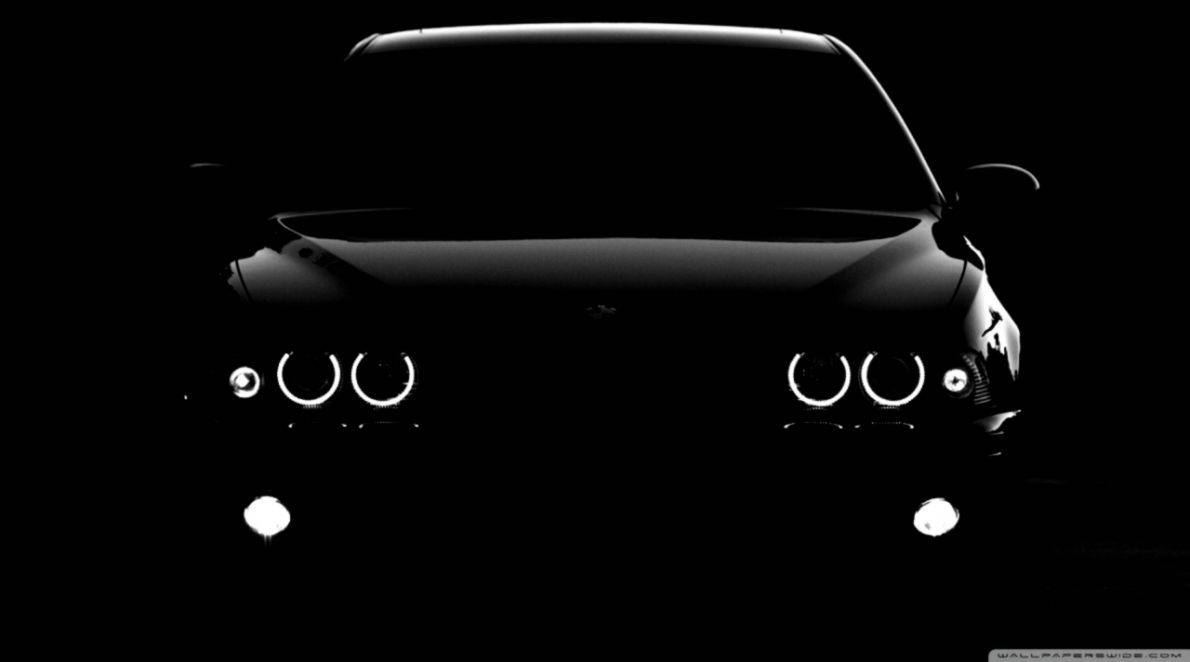
\includegraphics[width=0.4\textwidth]{BMW.jpg}
  \caption{Non-Floating mit [H].}
\end{figure}

\begin{figure}[htbp]
  % Floating (LaTeX entscheidet die beste Position)
  % LaTeX optimiert das Layout automatisch
  % Kann auf eine andere Seite verschoben werden
  % Vorteil: professionelleres Layout, weniger Leerraum
  % Nachteil: Abbildung kann weit vom Text entfernt sein
  \centering
  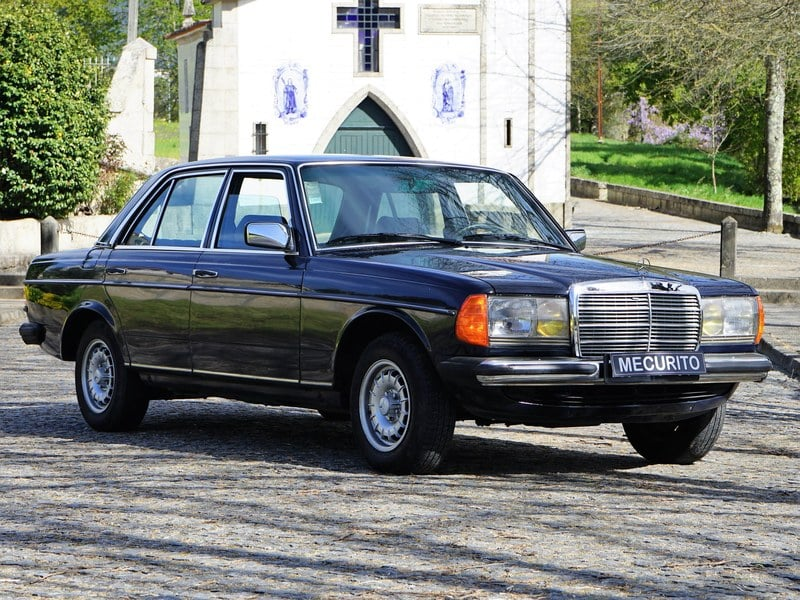
\includegraphics[width=0.4\textwidth]{Mercedes.jpg}
  \caption{Floating mit [htbp].}
\end{figure}

% =====================================================================
\subsection{Checkliste}
% Zusammenfassung wichtiger Hinweise für die Arbeit mit Abbildungen
% =====================================================================

\subsubsection{Wichtige Hinweise}

\paragraph{Dateiformat:}
\begin{itemize}
  \item \textbf{Vektorgrafiken:} PDF, EPS (ideal für Diagramme, Logos)
  \item \textbf{Rastergrafiken:} PNG (für Screenshots), JPG (für Fotos)
  \item Vermeide BMP und TIFF (große Dateien)
\end{itemize}

\paragraph{Auflösung:}
\begin{itemize}
  \item Minimum: 300 DPI für Druckqualität
  \item Web/Bildschirm: 72-150 DPI ausreichend
\end{itemize}

\paragraph{Positionierungsoptionen:}
\begin{itemize}
  \item \texttt{[H]} = Genau hier (benötigt float-Paket)
  \item \texttt{[h]} = Hier bevorzugt
  \item \texttt{[t]} = Oben auf der Seite
  \item \texttt{[b]} = Unten auf der Seite
  \item \texttt{[p]} = Eigene Seite
  \item \texttt{[!]} = Ignoriert LaTeX-Restriktionen
\end{itemize}

\paragraph{Häufige Fehler:}
\begin{itemize}
  \item Dateiendung vergessen bei \texttt{\textbackslash includegraphics}
  \item Falsche Bildpfade (verwende relative Pfade)
  \item \texttt{\textbackslash centering} vergessen
  \item Zu große Bilder ohne Skalierung
  \item Labels vergessen bei Referenzierung
\end{itemize}




\cleardoublepage
%%%%%%%%%%%%%%%%%%%%%%%%%%%%%%%%%%%%%%%%%%%%%%%%%%%%%%%%%%%%%%%%%%%%%%
%                   ANFANG Literaturverzeichnis
%%%%%%%%%%%%%%%%%%%%%%%%%%%%%%%%%%%%%%%%%%%%%%%%%%%%%%%%%%%%%%%%%%%%%%
\section{Literaturverzeichnis Beispiel}
  %Beispielzitat, weil im Literaturverzeichnis sonst nichts steht:
  \noindent
  Methodisch wurde das mehrfach diskutiert \parencite{einstein1905,knuth1984,lamport1994}.

  \printbibliography %Druckt das Literaturverzeichnis am Ende des Dokuments

\end{document}

%%%%%%%%%%%%%%%%%%%%%%%%%%%%%%%%%%%%%%%%%%%%%%%%%%%%%%%%%%%%%%%%%%%%%%
%                   Zitiermöglichkeiten in LaTeX
%%%%%%%%%%%%%%%%%%%%%%%%%%%%%%%%%%%%%%%%%%%%%%%%%%%%%%%%%%%%%%%%%%%%%%

%Autor im Satz:
\textcite{einstein1905} entwickelt die Spezielle Relativitätstheorie.

%Klammerzitat:
Klammerzitat: Das \LaTeX{}-System ist weit verbreitet \parencite{lamport1994}.


%Seiten- und Stellenangaben:
Eine Seite: \parencite[23]{knuth1984}. \\
Bereich: \parencite[23--27]{knuth1984}. \\
Kapitel/Abbildung: \parencite[Kap.\,2; Abb.\,3]{lamport1994}.

%Meherere Quellen auf einmal:
Methodisch wurde das mehrfach diskutiert \parencite{einstein1905,knuth1984,lamport1994}.

%Fußnotenzitate:
Webressourcen lassen sich bequem als Fußnote setzen:\footnote{Vgl.\ \footcite{w3cHTML}.}

%Autor oder Jahr einzeln:
Nur Autor: \citeauthor{einstein1905}; nur Jahr: \citeyear{einstein1905}.
%================================================================================================================================================

%================================================================================================================================================
%Literaturverzeichnis anpassen 

%Eigene Überschrift für Literaturverzeichnis, Eintrag ins Inhaltsverzeichnis:
\printbibliography[title={Literatur}, heading=bibintoc]

%Teil-Literaturverzeichnis nach Typ:
\printbibliography[type=book,     title={Bücher}]
\printbibliography[type=article,  title={Zeitschriftenartikel}]
\printbibliography[type=online,   title={Webquellen}]

%Teil-Literaturverzeichnis nach Stichwort:
\printbibliography[keyword=seminar, title={Quellen für das Seminar}]

% Familienname zuerst anzeigen (in Preambel):
\DeclareNameAlias{default}{family-given}

%Eigene Kategorien (z.b: Klassiker):
\DeclareBibliographyCategory{klassiker}
\addtocategory{klassiker}{knuth1984,lamport1994}




%%%%%%%%%%%%%%%%%%%%%%%%%%%%%%%%%%%%%%%%%%%%%%%%%%%%%%%%%%%%%%%%%%%%%%
%                   Verzeichnisstruktur der Diplomarbeit
%%%%%%%%%%%%%%%%%%%%%%%%%%%%%%%%%%%%%%%%%%%%%%%%%%%%%%%%%%%%%%%%%%%%%%




% 
% Scorpion/
% ├── chapters/                   # Kapitel 
% │   ├── main.tex                      # Hauptdokument
% │   ├── preamble.tex                  # Pakete & Einstellungen
% │   ├── titlepage.tex                 # Titelblatt
% │   ├── KARS/                         # KARS's Ordner
% │   │   └── 03_KARS_teil.tex          # KARS's Teil
% │   ├── FUCJ/                         # FUCJ's Ordner
% │   ├── KASF/                         # KASF's Ordner
% │   ├── MAYF/                         # MAYF's Ordner
% │   └── SCHS/                         # SCHS's Ordner
% │
% ├── figures/                   # Alle Abbildungen
% │   ├── AllPics/                      # Gemeinsame Bilder
% │   │   ├── logo.png
% │   │   └── blockdiagramm.pdf
% │   ├── FUCJ/                         # FUCJ's Bilder
% │   ├── KARS/                         # KARS's Bilder
% │   ├── KASF/                         # KASF's Bilder
% │   ├── MAYF/                         # MAYF's Bilder
% │   └── SCHS/                         # SCHS's Bilder
% │
% ├── tables/                   # Tabellen als separate Dateien
% │   ├── messergebnisse.tex
% │   ├── vergleichstabelle.tex
% │   └── kostenaufstellung.tex
% │
% └── appendix/                 # Anhänge
%     ├── A_code.tex
%     ├── B_datenblätter.tex
%     └── C_messungen.tex
